% My scribes for all the lectures, in one document.
% Every lecture day has its own file in tex/ and starts with \newlecture{date}{topic}.
% scribe.sty is an unmodified copy of the course file.

\documentclass[a4paper,11pt,final]{article}
\usepackage{scribecompat} % must come before scribe
\usepackage{scribe}
\usepackage{scribeextras} % \newlecture, dashed exercise boxes, \solutionspace, inline TikZ

\begin{document}

%%%%%%%%%%%%%%%%%%%%%%%%%%%%%%%%%%%%%%%%%%%%%%%%%%%%%%%%%%%%%%%%%%%%%%%%%%%
% Document begins here %%%%%%%%%%%%%%%%%%%%%%%%%%%%%%%%%%%%%%%%%%%%%%%%%%%%
%%%%%%%%%%%%%%%%%%%%%%%%%%%%%%%%%%%%%%%%%%%%%%%%%%%%%%%%%%%%%%%%%%%%%%%%%%%

\begin{center}
\textbf{\large Quantum Computing} \\

Professor Gopal Pandurangan\\
\vspace{0.1in}
\end{center}

\hrule

\vspace{0.1in}

\textbf{Scribe Author:} Armaan Amatya

\vspace{0.1in}

\hrule

\vspace{0.1in}

\tableofcontents

%%%%%%%%%%%%%%%%%%%%%%%%%%%%%%%%%%%%%%%%%%%%%%%%%%%%%%%%%%%%%%%%%%%%%%%%%%%
% Lectures, in order. Append new lectures at the end. %%%%%%%%%%%%%%%%%%%%%
%%%%%%%%%%%%%%%%%%%%%%%%%%%%%%%%%%%%%%%%%%%%%%%%%%%%%%%%%%%%%%%%%%%%%%%%%%%

\newlecture{August 25, 2026}{Efficient Algorithms, Random Sampling, Lower Bound for
    Deterministic Search, Probability Basics}
In this first lecture, we see why randomness and quantum computation matter for two basic problems,
primality/factoring and search. We introduce random sampling as the basic primitive of randomized
algorithms, prove a lower bound of $n-1$ queries for deterministic search, and review the basics of
probability that we need for the rest of the course.

\section{Efficient Algorithms and Finding Prime Numbers}

Consider the problem of deciding whether a given number $n$ is prime. The input is the binary
representation of $n$, so the \emph{input size} is the number of bits $N = \log_2 n$.

\begin{definition}[Efficient Algorithm]
    An algorithm is \textbf{efficient} if it runs in time polynomial in the input size, i.e., in time
    $\bigO{N^k}$ for some constant $k$. For primality testing this means time
    $\bigO{(\log_2 n)^k}$.
\end{definition}

Trial division by all numbers up to $\sqrt{n}$ takes $\bigTh{\sqrt{n}} = \bigTh{2^{N/2}}$ time,
which is exponential in the input size. A deterministic polynomial-time algorithm exists
(time $\tilde{\mathcal{O}}(N^{12})$, later improved to $\tilde{\mathcal{O}}(N^{6})$),
but it is not used in practice.

\subsection{Randomized Algorithms}

The algorithm used in practice is \emph{randomized}. The Miller--Rabin test decides primality with
high probability in $\bigO{N^3}$ time. If $n$ is composite, then at least
$\sfrac{3}{4}$ of the numbers in $\set{2, \dots, n-2}$ are \emph{witnesses} of the fact that $n$ is
composite, while a prime has no witness. So after $k$ independent samples a composite $n$ goes
undetected with probability at most $\left(\sfrac{1}{4}\right)^k$: the answer ``composite'' is always
right, and the answer ``prime'' is wrong with probability at most $\left(\sfrac{1}{4}\right)^k$.

\section{Random Sampling}

All that a randomized algorithm needs is the ability to \emph{sample}. We assume that flipping a
(fair) coin is an $\bigO{1}$ time primitive.

\subsection{Sampling a Random Element of an Array}

Consider an array with $n$ slots (\cref{fig:coinflips-0825}), $n$ a power of $2$. Every index is a
bit string of $\log_2 n = \log n$ bits, so flipping one coin for each bit samples a uniformly random
element in $\bigO{\log n}$ time:
$\prob{\text{index $i$ is chosen}} = \left(\sfrac{1}{2}\right)^{\log n} = \sfrac{1}{n}$ for every $i$.

\begin{figure}[ht]
    \centering
    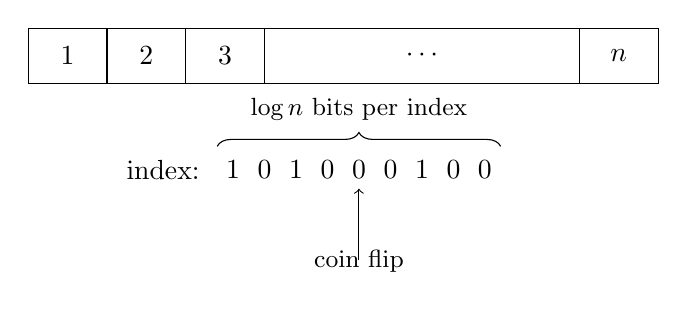
\begin{tikzpicture}
        % the array
        \draw (0,0) rectangle (8,0.7);
        \foreach \x in {1,2,3,7} {\draw (\x,0) -- (\x,0.7);}
        \node at (0.5,0.35) {$1$};
        \node at (1.5,0.35) {$2$};
        \node at (2.5,0.35) {$3$};
        \node at (5,0.35) {$\cdots$};
        \node at (7.5,0.35) {$n$};
        % an index, written as a bit string
        \node[anchor=east] at (2.3,-1.1) {index:};
        \foreach \x/\b in {0/1,1/0,2/1,3/0,4/0,5/0,6/1,7/0,8/0} {
                \node (b\x) at (2.6+0.4*\x,-1.1) {$\b$};
            }
        \draw[->] (b4.south) ++(0,-0.9) -- (b4.south);
        \node[below] at (4.2,-2.0) {\small coin flip};
        \draw[decorate, decoration={brace, amplitude=5pt}] (2.4,-0.8) -- (6.0,-0.8)
        node[midway, above=6pt] {\small $\log n$ bits per index};
    \end{tikzpicture}
    \caption{Each of the $\log n$ bits of the index is one coin flip.}
    \label{fig:coinflips-0825}
\end{figure}

We usually assume that an element can be sampled in constant time. This is only justified when the
space we sample from has polynomial size in $n$, since then the number of coin flips is
$\bigO{\log n}$.

\subsection{With and Without Replacement}

Random sampling can be done \emph{with} or \emph{without} replacement. We almost always analyze
sampling with replacement, since without replacement the samples are no longer independent.

Suppose that we are looking for one particular element of the array. Every sample hits it with
probability $\sfrac{1}{n}$, so sampling (with replacement) until it is found takes
$\expectation{\text{samples}} = \frac{1}{\sfrac{1}{n}} = n$ samples in expectation, and since the
samples are independent,
\[\prob{\text{not found after $k$ samples}} = \left(1 - \frac{1}{n}\right)^k,
    \qquad
    \prob{\text{found within $k$ samples}} = 1 - \left(1 - \frac{1}{n}\right)^k.\]

\section{Factoring}

Given $n = pq$ with $p, q$ prime, find $p$ and $q$. Factoring is an \emph{encryption primitive}: if
it can be solved quickly, then encryption based on it is broken. No polynomial-time (in
$N = \log n$) classical algorithm is known, but \emph{Shor's factoring algorithm} is a quantum
algorithm that runs in polynomial time $\bigO{N^3}$. There is \emph{no} known quantum algorithm that
solves \nptime-complete problems in polynomial time.

Recall that \nptime{} is the class of problems whose solutions can be verified in polynomial time,
and that the \nptime-complete problems are the \nptime{} problems to which every \nptime{} problem
reduces (equivalently, the problems that are reducible to 3-SAT and vice versa). Whether
$\textsc{P} = \nptime$ is open. A quantum computer can simulate a classical one with polynomial
overhead, so if quantum computers cannot solve \nptime-complete problems in polynomial time, then
$\textsc{P} \neq \nptime$.

\section{Search}

We are given an (unsorted) array $A$ with $n$ slots, which can only be accessed through
\emph{queries} (``what is $A[i]$?''), and we want to find the index of a given element $x$. A
sorted array allows binary search with $\bigO{\log n}$ queries. Linear search makes $\bigO{n}$
queries.

\subsection{Lower Bound for Deterministic Algorithms}

An upper bound needs one algorithm, but a lower bound of $\bigOm{f(n)}$ has to hold for \emph{all}
algorithms. We use an \emph{adversary argument}: given any algorithm, the adversary constructs an
input on which the algorithm performs badly.

\begin{theorem}[Lower Bound for Deterministic Search]\label{thm:detsearch-0825}
    Every deterministic algorithm for search makes at least $n - 1$ queries in the worst case.
\end{theorem}

\begin{proof}
    Fix a deterministic algorithm. The adversary does not fix the input in advance: whenever the
    algorithm queries a slot $i$, it answers that $A[i] \neq x$ (and fills $A[i]$ with some other
    value). Since the algorithm is deterministic, its $\nth{k}$ query is determined by the answers
    to the first $k-1$ queries, so this defines one run of the algorithm. Suppose that it stops
    after $k \leq n - 2$ queries and outputs an index $j$. At least $n - k \geq 2$ slots have not
    been queried, so the adversary can place $x$ in an unqueried slot different from $j$. The
    resulting array is consistent with all the answers given, and the algorithm is wrong on it. So a correct
    algorithm makes at least $n - 1$ queries.
\end{proof}

\subsection{Randomized and Quantum Algorithms}

The adversary argument breaks down for \emph{randomized} algorithms, because the queries are no
longer determined by the previous answers. Still, randomized search needs $\bigOm{n}$ expected
queries, by \emph{Yao's min-max principle} (next lecture). Grover's quantum algorithm solves search
with $\bigO{\sqrt{n}}$ queries (later in the course).

To show a \emph{quantum advantage} (also called quantum supremacy) for a problem, we have to
show that it needs $\bigOm{f(n)}$ queries classically but only $\littleO{f(n)}$ queries
quantumly.

\section{Probability}

A \textbf{sample space} $S$ is a finite set of \emph{simple events}, $\abs{S} = n$. A
\textbf{probability function} $\Pr \colon S \to [0,1] \subseteq \mathbb{R}$ assigns a probability to every
simple event. An \textbf{event} is a subset $A \subseteq S$, with probability
$\prob{A} = \sum_{a \in A} \prob{a}$. The probability function satisfies the \emph{axioms}
$\prob{A} \geq 0$ for every event $A$, $\prob{S} = 1$, and
$\prob{A_1 \cup A_2 \cup \dots \cup A_n} = \sum_{i=1}^{n} \prob{A_i}$ for pairwise disjoint events
$A_1, \dots, A_n$ (i.e., $A_i \cap A_j = \emptyset$ for all $i \neq j$). A \textbf{random variable} is a
function $X \colon S \to V$ from the sample space to a set of values $V$ (usually $V \subseteq \mathbb{R}$),
and for a value $r \in V$, $\prob{X = r} = \sum_{s \in S \,:\, X(s) = r} \prob{s}$.


\newlecture{September 1, 2026}{Query Complexity of Search, Coupon Collector Problem,
    Lower Bound for Randomized Algorithms, Chernoff Bounds}
In this lecture, we study the query complexity of search for classical randomized algorithms.
We analyze random sampling, relate it to the coupon collector problem, state a lower bound
for randomized search algorithms using Yao's minmax principle, and introduce Chernoff bounds.

\section{Query Complexity for Search}

We are given an array of $n$ slots (\cref{fig:array}). The array can only be accessed through
\emph{queries}: a query to a slot $x$ returns the value $f(x)$. In the \emph{search} problem, the goal
is to find the slot $x$ such that
\[f(x) = 1.\]
The cost of an algorithm is its \emph{query complexity}, i.e., the number of queries that it makes.

\begin{figure}[ht]
    \centering
    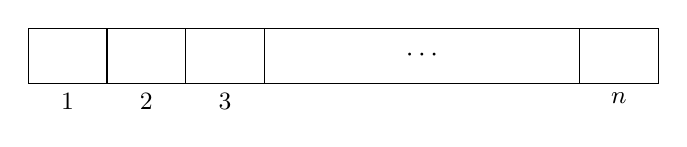
\begin{tikzpicture}
        \draw (0,0) rectangle (8,0.7);
        \foreach \x in {1,2,3,7} {\draw (\x,0) -- (\x,0.7);}
        \node at (5,0.35) {$\cdots$};
        \node[below] at (0.5,0) {\small $1$};
        \node[below] at (1.5,0) {\small $2$};
        \node[below] at (2.5,0) {\small $3$};
        \node[below] at (7.5,0) {\small $n$};
    \end{tikzpicture}
    \caption{An array of $n$ slots. We want to find the slot $x$ with $f(x) = 1$.}
    \label{fig:array}
\end{figure}

\subsection{Monte Carlo and Las Vegas Algorithms}

\begin{definition}[Monte Carlo and Las Vegas Algorithms]
    A \textbf{Monte Carlo} algorithm is a randomized algorithm whose error probability is $> 0$.

    A \textbf{Las Vegas} algorithm is a randomized algorithm whose error probability is $= 0$.
\end{definition}

\subsection{Random Sampling}

Consider random sampling \emph{with replacement}: in every step we query a slot that is chosen
uniformly at random among the $n$ slots. For every query,
\[\prob{\text{Success}} = \frac{1}{n}.\]
The number of queries until the first success is a \emph{geometric} random variable with
parameter $\sfrac{1}{n}$. Hence
\[\expectation{\text{queries}} = n.\]

If random sampling is stopped after a fixed number of queries, then it is a Monte Carlo algorithm,
since it can fail to find the slot. If we keep sampling until the slot is found, then it is a Las Vegas
algorithm, and
\[\expectation{\text{queries until find}} = n.\]

\section{Coupon Collector Problem}

Suppose that we want to distinguish 2 binary arrays (\cref{fig:binaryarrays}). To do this with
random sampling, all the $n$ slots have to be accessed. The number of queries needed by random sampling
(with replacement) to access all the $n$ slots is the \emph{coupon collector problem}.
We show that
\[\expectation{\text{queries}} \leq \bigO{n \log n}
    \quad\text{and}\quad
    \expectation{\text{queries}} \geq \bigOm{n \log n},\]
i.e., $\expectation{\text{queries}} = \bigTh{n \log n}$.

\begin{figure}[ht]
    \centering
    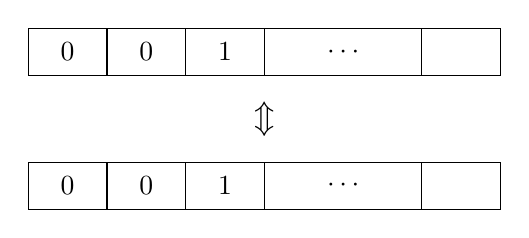
\begin{tikzpicture}
        % first array
        \draw (0,1.7) rectangle (6,2.3);
        \foreach \x in {1,2,3,5} {\draw (\x,1.7) -- (\x,2.3);}
        \node at (0.5,2.0) {$0$};
        \node at (1.5,2.0) {$0$};
        \node at (2.5,2.0) {$1$};
        \node at (4,2.0) {$\cdots$};
        % arrow between the arrays
        \node at (3,1.15) {\large $\Updownarrow$};
        % second array
        \draw (0,0) rectangle (6,0.6);
        \foreach \x in {1,2,3,5} {\draw (\x,0) -- (\x,0.6);}
        \node at (0.5,0.3) {$0$};
        \node at (1.5,0.3) {$0$};
        \node at (2.5,0.3) {$1$};
        \node at (4,0.3) {$\cdots$};
    \end{tikzpicture}
    \caption{To distinguish 2 binary arrays.}
    \label{fig:binaryarrays}
\end{figure}

\begin{theorem}[Coupon Collector]\label{thm:coupon}
    Let $X$ be the number of queries made by random sampling (with replacement) until all the
    $n$ slots are accessed. Then
    \[\expectation{X} = n H_n = \bigTh{n \log n},\]
    where $H_n = \sum_{i=1}^{n} \frac{1}{i}$ is the $\nth{n}$ harmonic number.
\end{theorem}

\begin{proof}
    Write
    \[X = X_1 + X_2 + \dots + X_n,\]
    where $X_i$ is the number of queries made to access a new slot, after $i-1$ different slots
    have already been accessed. When $i-1$ slots have been accessed, a query accesses a new slot
    with probability $\frac{n-(i-1)}{n}$. Hence $X_i$ is a geometric random variable,
    \[X_i \sim G\left(\frac{n-(i-1)}{n}\right),
        \qquad
        \expectation{X_i} = \frac{n}{n-(i-1)}.\]
    By linearity of expectation,
    \begin{align*}
        \expectation{X}
         & = \expectation{X_1 + X_2 + \dots + X_n} \\
         & = \sum_{i=1}^{n} \expectation{X_i}      \\
         & = \sum_{i=1}^{n} \frac{n}{n-(i-1)}      \\
         & = n \sum_{i=1}^{n} \frac{1}{n-i+1}      \\
         & = n H_n.
    \end{align*}
    Since $H_n = \bigTh{\log n}$, we get $\expectation{X} = \bigTh{n \log n}$.
\end{proof}

\newpage
\section{High Probability Bound}

The following was given in class as an exercise.

% Dashed box in my notes: exercise given in class.
\begin{exercise}
    Show that
    \[\prob{\text{any slot is accessed} \leq c \log n \text{ times}} \leq \frac{1}{n^2}.\]
\end{exercise}
\solutionspace % TODO: replace with \begin{proof} ... \end{proof}

The expectation of the number of queries is $\bigTh{n \log n}$. We now show that
$3 n \log n$ queries are enough with high probability. Here $\log$ is the natural logarithm.

\begin{theorem}\label{thm:whp}
    If random sampling makes $3 n \log n$ queries, then
    \[\prob{\text{fail}} \leq \frac{1}{n^2},
        \qquad\text{i.e.,}\qquad
        \prob{\text{Success}} \geq 1 - \frac{1}{n^2},\]
    where ``fail'' means that some slot is not accessed.
\end{theorem}

\begin{proof}
    Let $B_i$ be the event that slot $i$ is not accessed. A query does not access slot $i$ with
    probability $1 - \frac{1}{n}$. Using $1 - x \leq e^{-x}$,
    \begin{align*}
        \prob{B_i} = \prob{\text{slot $i$ not accessed}}
         & \leq \left(1 - \frac{1}{n}\right)^{3 n \log n} \\
         & \leq e^{-\frac{1}{n} \cdot 3 n \log n}         \\
         & = e^{-3 \ln n}                                  \\
         & = \frac{1}{n^3}.
    \end{align*}
    By the union bound,
    \[\prob{\bigcup_{i} B_i} \leq \sum_{i=1}^{n} \prob{B_i} = \frac{n}{n^3} = \frac{1}{n^2}.\]
\end{proof}

\section{Lower Bound for Randomized Algorithms}

\begin{theorem}\label{thm:lowerbound}
    Any Las Vegas randomized algorithm for search needs $\bigOm{n}$ expected queries.
\end{theorem}

The lower bound is shown using Yao's minmax principle.

\subsection*{Yao's Minmax Principle}

Let $A^{\mathrm{rand}}$ be a randomized algorithm, and let $\expectation{A^{\mathrm{rand}}}$ be its
expected number of queries. Let $\mu$ be a probability distribution over the inputs, and let
$D^{\mathrm{best}}_{\mu}$ be the best deterministic algorithm for inputs that are chosen according
to $\mu$. Then
\[\expectation{A^{\mathrm{rand}}}
    \geq \max_{\mu} \operatorname{\mathbb{E}}_{\mu}\left[D^{\mathrm{best}}_{\mu}\right]
    \geq \bigOm{n}.\]
The quantity $\operatorname{\mathbb{E}}_{\mu}\left[D^{\mathrm{best}}_{\mu}\right]$ is called the
\emph{distributional complexity}.

\section{Chernoff Bounds}

Let's say that a coin gives heads ($H$) with probability $\frac{1}{2} + \eps$ and tails ($T$) with
probability $\frac{1}{2} - \eps$. If we toss the coin $n$ times, then
\[\expectation{\text{Heads}} = n\left(\frac{1}{2} + \eps\right) = \frac{n}{2} + n\eps.\]
Chernoff bounds show that the number of heads is close to its expectation, so that
\[\prob{\text{Heads} < \frac{n}{2}} \sim \text{very small}.\]

In general, let
\[X = \sum_{i=1}^{n} X_i,
    \qquad
    X_i = \begin{cases}
        1 & \text{with probability } p_i,     \\
        0 & \text{with probability } 1 - p_i,
    \end{cases}\]
where the $X_i$ are independent Bernoulli random variables. If $p_i = p$ for all $i$, then
\[\expectation{X} = np, \qquad \variance{X} = np(1-p).\]
The distribution of $X$ is concentrated around its mean $np$ (\cref{fig:concentration}).

\begin{figure}[ht]
    \centering
    \begin{tikzpicture}
        % axes
        \draw[->] (-0.3,0) -- (8,0);
        \draw[->] (0,-0.2) -- (0,3.2);
        % distribution of X
        \draw[thick, domain=0:7.5, smooth, samples=120]
        plot (\x, {2.6*exp(-(\x-1.5)*(\x-1.5)/1.3)});
        % ticks
        \foreach \x/\l in {0.5/{\frac{1}{3}np}, 1.5/{np}, 4.5/{3np}, 7.5/{n}} {
                \draw (\x,0.08) -- (\x,-0.08) node[below] {\small $\l$};
            }
        \node[below left] at (0,0) {\small $0$};
        \draw[dashed] (4.5,0) -- (4.5,1.2);
    \end{tikzpicture}
    \caption{The distribution of $X$ is concentrated around the mean $np$.}
    \label{fig:concentration}
\end{figure}

\begin{theorem}[Chernoff Bounds]\label{thm:chernoff-0901}
    Let $X = \sum_{i=1}^{n} X_i$ be as above and let $\mu = \expectation{X}$.
    \begin{itemize}
        \item Upper tail (UI): for $0 < \delta < 1$,
              \[\prob{X \geq (1+\delta)\mu} \leq e^{-\frac{\mu \delta^2}{3}}.\]
        \item For $R \geq 6\mu$,
              \[\prob{X \geq R} \leq \frac{1}{2^R}.\]
        \item Lower tail (LI): for $0 < \delta < 1$,
              \[\prob{X \leq (1-\delta)\mu} \leq e^{-\frac{\mu \delta^2}{2}}.\]
    \end{itemize}
\end{theorem}


\newlecture{September 3, 2026}{Markov, Chebyshev and Chernoff Inequalities, Search,
    Birthday Paradox}
In this lecture, we state and prove Markov's inequality and Chebyshev's inequality, and we state the
Chernoff bound. We then look at the query complexity of search for classical and quantum algorithms,
and we analyze the birthday paradox.

\section{Markov's Inequality}

Markov's inequality uses only the expectation $\expectation{X}$ of the random variable, which is
also called the \emph{first moment}.

\begin{theorem}[Markov's Inequality]\label{thm:markov}
    Let $X \geq 0$ be a random variable. Then, for any $a > 0$,
    \[\prob{X \geq a \expectation{X}} \leq \frac{1}{a}.\]
    Equivalently, for any $b > 0$,
    \[\prob{X \geq b} \leq \frac{\expectation{X}}{b}.\]
\end{theorem}

\begin{figure}[ht]
    \centering
    \begin{tikzpicture}
        \draw (0,0) -- (8,0);
        \draw (0,0.1) -- (0,-0.1) node[below] {\small $0$};
        \draw (3,0.1) -- (3,-0.1);
        \node[above] at (3,0.1) {\small $\mu = \expectation{X}$};
        \draw (6,0.1) -- (6,-0.1) node[below] {\small $a\mu$};
        \draw[decorate, decoration={brace, amplitude=5pt}] (6,0.25) -- (8,0.25)
        node[midway, above=6pt] {\small $\leq \frac{1}{a}$};
    \end{tikzpicture}
    \caption{Markov's inequality: the probability that $X$ is at least $a\mu$ is at most $\sfrac{1}{a}$.}
    \label{fig:markov}
\end{figure}

\begin{proof}
    Let
    \[I = \begin{cases}
            1 & \text{if } X \geq b, \\
            0 & \text{otherwise.}
        \end{cases}\]
    Then
    \[I \leq \frac{X}{b}.\]
    This is true for $X \geq b$, since then $I = 1 \leq \frac{X}{b}$. It is also true for $X < b$,
    since then $I = 0$ and $X \geq 0$.
    Markov's inequality follows by taking expectations on both sides:
    \[\expectation{I} \leq \expectation{\frac{X}{b}} = \frac{\expectation{X}}{b}.\]
    Since
    \[\prob{I = 1} = \prob{X \geq b} \qquad\text{and}\qquad \prob{I = 0} = \prob{X < b},\]
    we have $\expectation{I} = \prob{I = 1}$, and hence
    \[\prob{X \geq b} \leq \frac{\expectation{X}}{b}.\]
    Taking $b = a \expectation{X}$ gives $\prob{X \geq a \expectation{X}} \leq \frac{1}{a}$.
\end{proof}

\section{Chebyshev's Inequality}

Chebyshev's inequality uses the variance of the random variable, which is also called the
\emph{second moment}.

\begin{definition}[Variance and Standard Deviation]
    The \textbf{variance} of a random variable $X$ is
    \[\variance{X} = \expectation{\left(X - \expectation{X}\right)^2}.\]
    The \textbf{standard deviation} of $X$ is
    \[\sigma = \sqrt{\variance{X}}.\]
\end{definition}

\begin{theorem}[Chebyshev's Inequality]\label{thm:chebyshev}
    For any random variable $X$ and any $a > 0$,
    \[\prob{\abs{X - \expectation{X}} \geq a} \leq \frac{\variance{X}}{a^2} = \frac{\sigma^2}{a^2}.\]
\end{theorem}

Here $\abs{X - \expectation{X}}$ is the deviation of $X$ from its mean.

\begin{proof}
    \[\prob{\abs{X - \expectation{X}} \geq a}
        = \prob{\left(X - \expectation{X}\right)^2 \geq a^2}
        \leq \frac{\expectation{\left(X - \expectation{X}\right)^2}}{a^2}
        = \frac{\variance{X}}{a^2},\]
    where the inequality is Markov's inequality applied to the random variable
    $\left(X - \expectation{X}\right)^2 \geq 0$.
\end{proof}

\section{Chernoff Bound}

The Chernoff bounds of the last lecture (\cref{thm:chernoff-0901}) were restated in class with the
independence assumption made explicit. For a sum $X = \sum_{i=1}^{n} X_i$ of \emph{mutually
independent} indicator random variables with $\prob{X_i = 1} = p_i$, linearity of expectation gives
$\mu = \expectation{X} = \sum_{i=1}^{n} p_i$, and for $0 < \delta < 1$
\[\prob{X \geq (1+\delta)\mu} \leq e^{-\frac{\mu \delta^2}{3}},
    \qquad
    \prob{X < (1-\delta)\mu} \leq e^{-\frac{\mu \delta^2}{2}},\]
and $\prob{X \geq R} \leq 2^{-R}$ for $R \geq 6\mu$.

\section{Search}

Let $f \colon D \to R$ be a function from a domain $D$ to a range $R$ (\cref{fig:function}).
Given $y$, we ask: is there an $x$ such that $f(x) = y$? We consider
\[f \colon [1, \dots, N] \to [1, \dots, N],\]
and we want to find an $x$ such that $f(x) = k$. The function can be seen as an array with $n$
slots, where $n$ is the size of the domain, and the cost of an algorithm is the number of queries
to $f$.

\begin{figure}[ht]
    \centering
    \begin{tikzpicture}
        % array
        \draw (0,0) rectangle (6,0.7);
        \foreach \x in {1,2,4,5} {\draw (\x,0) -- (\x,0.7);}
        \node at (3,0.35) {$\cdots$};
        \node[below] at (0.5,0) {\small $1$};
        \node[below] at (5.5,0) {\small $n$};
        % function from D to R
        \draw (8.5,0.35) ellipse (0.6 and 1);
        \draw (11.5,0.35) ellipse (0.6 and 1);
        \node at (8.5,1.65) {$D$};
        \node at (11.5,1.65) {$R$};
        \node[point] (y) at (11.5,0.35) {};
        \foreach \h in {0.95,0.35,-0.25} {
                \node[point] (x) at (8.5,\h) {};
                \draw[->] (x) -- (y);
            }
        \node at (10,1.35) {$f$};
    \end{tikzpicture}
    \caption{Left: an array with $n$ slots. Right: a function $f \colon D \to R$.}
    \label{fig:function}
\end{figure}

\begin{itemize}
    \item Randomized classical algorithm: $\bigTh{n}$ queries.
    \item Grover's algorithm: $\bigO{\sqrt{n}}$ queries.
\end{itemize}

For the random sampling algorithm,
\[\expectation{\text{queries}} = \bigO{n}, \qquad \prob{\text{Success}} = \frac{1}{n}.\]

\paragraph{Probability amplitude amplification.} If the classical success probability is $p$, then
in the quantum case it becomes $\sqrt{p}$.

\section{Birthday Paradox}

There are $m$ people and $n$ birthdays ($n = 365$). We are looking for a \emph{collision}, i.e.,
$x \neq y$ such that
\[f(x) = f(y),\]
where $f(x)$ is the birthday of person $x$.

Let $E_i$ be the event that the $\nth{i}$ birthday is different from the first $i-1$ birthdays. Then
\begin{align*}
    \prob{\bigcap_{i=1}^{m} E_i}
     & = \prob{\text{all birthdays different}}                                                                        \\
     & = \prob{E_1} \cdot \prob{E_2 \given E_1} \cdot \prob{E_3 \given E_2 \cap E_1} \cdots                           \\
     & = 1 \cdot \left(1 - \frac{1}{n}\right) \cdot \left(1 - \frac{2}{n}\right) \cdots \left(1 - \frac{m-1}{n}\right) \\
     & = \prod_{i=0}^{m-1} \left(1 - \frac{i}{n}\right)                                                                \\
     & \leq \prod_{i=0}^{m-1} e^{-\sfrac{i}{n}}                                                                        \\
     & = e^{-\sum_{i=0}^{m-1} \frac{i}{n}}                                                                             \\
     & = e^{-\frac{(m-1)m}{2n}}.
\end{align*}
For $m = \sqrt{2n} + 1$,
\[\prob{\text{all birthdays different}}
    \leq e^{-\frac{\sqrt{2n}\left(\sqrt{2n}+1\right)}{2n}}
    \leq e^{-\frac{2n}{2n}}
    = \frac{1}{e}
    \leq \frac{1}{2}.\]
Hence $\bigO{\sqrt{n}}$ people are enough to have a constant probability of collision.

\subsection{Expected Number of Collisions}

The birthday paradox can be seen as throwing $m$ balls into $n$ bins (\cref{fig:ballsbins}).
We show that for $m \approx \sqrt{2n}$,
\[\expectation{\text{\# collisions}} \geq 1.\]

\begin{figure}[ht]
    \centering
    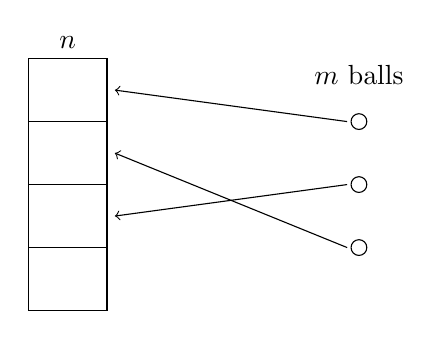
\begin{tikzpicture}
        % bins
        \draw (0,0) rectangle (1,3.2);
        \foreach \y in {0.8,1.6,2.4} {\draw (0,\y) -- (1,\y);}
        \node[above] at (0.5,3.2) {$n$};
        % balls
        \node[above] at (4.2,2.75) {$m$ balls};
        \foreach \b/\t in {2.4/2.8, 1.6/1.2, 0.8/2.0} {
                \draw (4.2,\b) circle (0.1);
                \draw[->] (4.05,\b) -- (1.1,\t);
            }
    \end{tikzpicture}
    \caption{$m$ balls are thrown into $n$ bins.}
    \label{fig:ballsbins}
\end{figure}

Let $X$ be the number of collisions. $X$ takes values from $0$ to $\binom{m}{2}$. Write
\[X = \sum_{i \neq j} X_{ij},
    \qquad
    X_{ij} = \begin{cases}
        1 & \text{if } f(i) = f(j), \\
        0 & \text{else,}
    \end{cases}\]
where the sum is over the $\binom{m}{2}$ pairs $i \neq j$. The random variables $X_{ij}$ are
\emph{pairwise independent}. By linearity of expectation,
\begin{align*}
    \expectation{X}
     & = \sum_{i \neq j} \expectation{X_{ij}} \\
     & = \sum_{i \neq j} \prob{X_{ij} = 1}    \\
     & = \sum_{i \neq j} \frac{1}{n}          \\
     & = \binom{m}{2} \frac{1}{n}
    = \frac{m(m-1)}{2n}
    \sim \frac{m^2}{2n}
    = \bigTh{\frac{m^2}{n}}.
\end{align*}

% Dashed box in my notes: exercise given in class.
\begin{exercise}\label{ex:birthday-0903}
    Show that
    \[\prob{X \geq 1} \geq \bigTh{1},\]
    i.e., the birthday paradox occurs.
\end{exercise}

The hint given in class is to compute the variance
\[\variance{X} = \variance{\sum_{i \neq j} X_{ij}}\]
and to use Chebyshev's inequality (\cref{thm:chebyshev}): if the variance of $X$ is small compared
to $\expectation{X}^2$, then $X$ is rarely far from its mean, and in particular rarely $0$. We first
prove the claim that the $X_{ij}$ are pairwise independent, which is what makes the variance easy
to compute.

\begin{lemma}[Variance of the Number of Collisions]\label{lem:pairwise-0903}
    For any two different pairs $\set{i,j} \neq \set{k,l}$,
    \[\expectation{X_{ij} X_{kl}} = \expectation{X_{ij}} \expectation{X_{kl}} = \frac{1}{n^2},\]
    i.e., $X_{ij}$ and $X_{kl}$ are independent. Consequently
    \[\variance{X} = \sum_{i \neq j} \variance{X_{ij}}
        = \binom{m}{2} \frac{1}{n} \left(1 - \frac{1}{n}\right) \leq \expectation{X}.\]
\end{lemma}

\begin{proof}
    Since $X_{ij} X_{kl} = 1$ exactly when both indicators are $1$,
    \[\expectation{X_{ij} X_{kl}} = \prob{f(i) = f(j) \text{ and } f(k) = f(l)}.\]
    There are two cases.
    \begin{itemize}
        \item The pairs are disjoint, $\set{i,j} \cap \set{k,l} = \emptyset$. Then the two events
              depend on the birthdays of four different people, which are independent, so the
              probability is $\prob{f(i) = f(j)} \cdot \prob{f(k) = f(l)} = \sfrac{1}{n^2}$.
        \item The pairs share one person, say $\set{i,j}$ and $\set{i,k}$ with $j \neq k$. The
              birthdays $f(j)$ and $f(k)$ are independent of $f(i)$ and of each other, and each
              equals a given day $b$ with probability $\sfrac{1}{n}$, so
              \[\prob{f(j) = f(i) \text{ and } f(k) = f(i)}
                  = \sum_{b=1}^{n} \prob{f(i) = b} \cdot \frac{1}{n} \cdot \frac{1}{n}
                  = \frac{1}{n^2}.\]
    \end{itemize}
    In both cases $\expectation{X_{ij} X_{kl}} = \sfrac{1}{n^2} = \expectation{X_{ij}} \expectation{X_{kl}}$.
    For two indicator random variables this is the same as independence, since their joint
    distribution is determined by $\prob{X_{ij} = 1}$, $\prob{X_{kl} = 1}$ and $\prob{X_{ij} = X_{kl} = 1}$.

    For the variance, write $X - \expectation{X} = \sum_{i \neq j} \left(X_{ij} - \expectation{X_{ij}}\right)$
    and expand the square:
    \begin{align*}
        \variance{X}
         & = \expectation{\Big(\sum_{i \neq j} \left(X_{ij} - \expectation{X_{ij}}\right)\Big)^2}                                                           \\
         & = \sum_{i \neq j} \expectation{\left(X_{ij} - \expectation{X_{ij}}\right)^2}
        + \sum_{\set{i,j} \neq \set{k,l}} \expectation{\left(X_{ij} - \expectation{X_{ij}}\right) \left(X_{kl} - \expectation{X_{kl}}\right)} \\
         & = \sum_{i \neq j} \variance{X_{ij}}
        + \sum_{\set{i,j} \neq \set{k,l}} \left(\expectation{X_{ij} X_{kl}} - \expectation{X_{ij}} \expectation{X_{kl}}\right)
        = \sum_{i \neq j} \variance{X_{ij}},
    \end{align*}
    where the second sum vanishes by the first part. Finally $X_{ij}$ is an indicator with
    $\prob{X_{ij} = 1} = \sfrac{1}{n}$, so $X_{ij}^2 = X_{ij}$ and
    \[\variance{X_{ij}} = \expectation{X_{ij}^2} - \expectation{X_{ij}}^2
        = \frac{1}{n} - \frac{1}{n^2} = \frac{1}{n} \left(1 - \frac{1}{n}\right) \leq \frac{1}{n}.\]
    Summing over the $\binom{m}{2}$ pairs gives $\variance{X} \leq \binom{m}{2} \frac{1}{n} = \expectation{X}$.
\end{proof}

\begin{theorem}[The Birthday Paradox Occurs]\label{thm:birthday-0903}
    If $m \geq 2\sqrt{n} + 1$, then
    \[\prob{X \geq 1} \geq \frac{1}{2}.\]
    In words: with $\bigO{\sqrt{n}}$ people there is a collision with constant probability.
\end{theorem}

\begin{proof}
    The event $X = 0$ (no collision) is contained in the event $\abs{X - \expectation{X}} \geq \expectation{X}$,
    since $X = 0$ means $X - \expectation{X} = -\expectation{X}$. By Chebyshev's inequality
    (\cref{thm:chebyshev}) with $a = \expectation{X}$, and then \cref{lem:pairwise-0903},
    \[\prob{X = 0} \leq \prob{\abs{X - \expectation{X}} \geq \expectation{X}}
        \leq \frac{\variance{X}}{\expectation{X}^2} \leq \frac{\expectation{X}}{\expectation{X}^2} = \frac{1}{\expectation{X}}.\]
    For $m \geq 2\sqrt{n} + 1$, since $m(m-1)$ grows with $m$,
    \[\expectation{X} = \frac{m(m-1)}{2n} \geq \frac{(2\sqrt{n} + 1) \cdot 2\sqrt{n}}{2n}
        = \frac{4n + 2\sqrt{n}}{2n} \geq 2,\]
    so $\prob{X = 0} \leq \sfrac{1}{2}$, and $\prob{X \geq 1} = 1 - \prob{X = 0} \geq \sfrac{1}{2}$.
\end{proof}

The direct computation of $\prob{\text{all birthdays different}}$ above already gave
$\prob{X = 0} \leq \sfrac{1}{e}$ for $m = \sqrt{2n} + 1$. The point of this \emph{second moment}
argument is that it only uses $\expectation{X}$ and $\variance{X}$, so it also works when the exact
probability cannot be computed.

\section{Quantum Birthday Paradox}

The birthday paradox, seen as an algorithm, solves the \emph{collision problem}: given query access
to a function $f$, find $x \neq y$ with $f(x) = f(y)$. Querying $m = \sqrt{2n} + 1$ random points finds
a collision with probability at least $\sfrac{1}{2}$, so $\bigO{\sqrt{n}}$ queries suffice classically.
The quantum version of the problem is studied later in the course; here we show that classically
$\sqrt{n}$ queries are also necessary. An algorithm makes $k$ queries
\[f(x_1), \dots, f(x_k),\]
where the point $x_s$ may depend on the earlier answers $f(x_1), \dots, f(x_{s-1})$ and on random coins.

% Not in a dashed box in my notes, but written as something to show.
\begin{exercise}\label{ex:collision-lb-0903}
    Show a $\sqrt{n}$ lower bound in the classical case.
\end{exercise}

We use the same model as in the birthday paradox: $f \colon D \to [n]$, where $[n] = \set{1, \dots, n}$,
is a \emph{random function}, i.e., every value $f(x)$ is uniform in $[n]$ and independent of all the
other values (the birthday of person $x$). The algorithm \emph{finds a collision} if it outputs
$x \neq y$ with $f(x) = f(y)$. We may assume that the algorithm queries the two points that it
outputs: if it does not, it can do so with at most $2$ extra queries, which does not change the
bound below. We may also assume that the $k$ queried points are different, since repeating a query
gives no new information.

\begin{theorem}[Classical Lower Bound for Collision Finding]\label{thm:collision-lb-0903}
    Let $f \colon D \to [n]$ be a random function. Every classical algorithm (deterministic or
    randomized, adaptive) that makes $k$ queries finds a collision with probability at most
    \[\frac{\binom{k}{2}}{n} = \frac{k(k-1)}{2n}.\]
    In particular, to find a collision with probability at least $\sfrac{1}{2}$ it needs
    $k > \sqrt{n}$ queries, so the classical query complexity of the collision problem is $\bigOm{\sqrt{n}}$.
\end{theorem}

\begin{proof}
    Since the algorithm queries the points that it outputs, it can only find a collision if two of
    its queried values agree. Let $E_s$ be the event that the $\nth{s}$ query collides with an earlier
    one, i.e., $f(x_s) \in \set{f(x_1), \dots, f(x_{s-1})}$. A collision among the $k$ queries means
    that some $E_s$ occurs, so by the union bound
    \[\prob{\text{collision}} \leq \sum_{s=1}^{k} \prob{E_s}.\]
    We claim that $\prob{E_s} \leq \frac{s-1}{n}$. Consider the moment just before the $\nth{s}$
    query. The algorithm chooses $x_s$ from the $s-1$ answers seen so far and from its random coins;
    condition on all of these. Then $x_s$ is a fixed point that has not been queried before, so its
    value $f(x_s)$ is still a uniformly random element of $[n]$, independent of the $s-1$ values
    $f(x_1), \dots, f(x_{s-1})$, which are now fixed. The probability that $f(x_s)$ equals one of these
    $s-1$ fixed values is therefore at most $\frac{s-1}{n}$, no matter how the algorithm chose $x_s$.
    Since this holds for every outcome of the first $s-1$ steps, it also holds without conditioning,
    which proves the claim. Hence
    \[\prob{\text{collision}} \leq \sum_{s=1}^{k} \frac{s-1}{n} = \frac{0 + 1 + \dots + (k-1)}{n} = \frac{k(k-1)}{2n}.\]
    If the algorithm succeeds with probability at least $\sfrac{1}{2}$, then $\frac{k(k-1)}{2n} \geq \frac{1}{2}$,
    i.e., $k^2 > k(k-1) \geq n$, so $k > \sqrt{n}$.
\end{proof}

\paragraph{Worst case inputs.} \cref{thm:collision-lb-0903} is a statement about a \emph{random}
input $f$: the distributional complexity of the collision problem under the uniform distribution on
functions is $\bigOm{\sqrt{n}}$. By Yao's minmax principle from the lecture of September~1 (in its
version for algorithms that are allowed to err), this is also a lower bound for every randomized
algorithm on its worst case input. Together with the birthday paradox, which finds a collision with
$\bigO{\sqrt{n}}$ queries, the classical query complexity of finding a collision is $\bigTh{\sqrt{n}}$.


\newlecture{September 8, 2026}{Distributed Computing, Randomized Leader Election in a Complete
    Network, Random Walks, Law of Large Numbers}
In this lecture, we turn to distributed computing. We define the synchronous complete network model,
study the leader election problem, and analyze a randomized algorithm that elects a leader in $\bigO{1}$
rounds with only $\bigO{\sqrt{n} \log^{\sfrac{3}{2}} n}$ messages. We then take a first look at random
walks on undirected graphs, and we prove the weak law of large numbers with Chebyshev's inequality.

\section{Distributed Computing in a Complete Network}

The network is a \emph{complete graph} $G$ on $n$ nodes (\cref{fig:network-0908}). Every pair of nodes
is joined by a bidirectional communication link, so there are $\binom{n}{2} = \frac{n(n-1)}{2}$ edges
and every node has $n - 1$ incident edges. The network is \emph{synchronous}: all nodes share a clock,
and the computation proceeds in \emph{rounds}. In one round, every node receives the messages sent
to it in the previous round, does a local computation, and sends messages on some of its edges
(receives $\to$ computes $\to$ sends).

\begin{figure}[ht]
    \centering
    \begin{tikzpicture}[scale=0.82]
        % complete network
        \node[point, label=above left:{\small $1$}] (a1) at (-1.3,0.9) {};
        \node[point, label=above:{\small $2$}] (a2) at (0,1.8) {};
        \node[point, label=above right:{\small $3$}] (a3) at (1.3,0.9) {};
        \node[point, label=below right:{\small $n-1$}] (a4) at (0.8,-0.6) {};
        \node[point, label=below left:{\small $n$}] (a5) at (-0.8,-0.6) {};
        \foreach \x/\y in {a1/a2, a1/a3, a1/a4, a1/a5, a2/a3, a2/a4, a2/a5, a3/a4, a3/a5, a4/a5} {
                \draw (\x) -- (\y);
            }
        % candidates and referees
        \begin{scope}[xshift=6cm]
            \node[point, label=left:{\small $u$}] (u) at (0,1.3) {};
            \node[point, label=left:{\small $v$}] (v) at (0,-0.1) {};
            \foreach \i/\h in {1/1.9, 2/1.25, 3/0.6, 4/-0.05, 5/-0.7} {
                    \node[point] (r\i) at (3.2,\h) {};
                }
            \node[right] at (3.3,0.6) {\small $r$};
            \foreach \i in {1,2} {\draw[->, shorten >=2pt] (u) -- (r\i);}
            \foreach \i in {4,5} {\draw[->, shorten >=2pt] (v) -- (r\i);}
            % the two arrows into the common referee end slightly apart
            \draw[->, shorten >=2pt] (u) -- ([yshift=3pt]r3.west);
            \draw[->, shorten >=2pt] (v) -- ([yshift=-3pt]r3.west);
            \node at (0,2.4) {\small candidates};
            \node at (3.2,2.4) {\small referees};
        \end{scope}
    \end{tikzpicture}
    \caption{Left: the complete network on $n$ nodes. Right: candidates $u$ and $v$ with a common
        referee $r$.}
    \label{fig:network-0908}
\end{figure}

\subsection{Leader Election}

\begin{problem}[Leader Election]
    All nodes run the same algorithm. At the end, exactly one node must be
    in the state \emph{leader}, and all other nodes must be in the state \emph{non-leader}.
\end{problem}

The goals are to minimize the number of rounds and the total number of messages sent. The nodes are
either \emph{labelled}, i.e., every node has a unique id, or \emph{anonymous}, i.e., the nodes have
no ids and cannot be told apart.

\paragraph{The trivial algorithm.} With unique ids, every node sends its id to all other nodes in the
first round, and the node with the minimum id becomes the leader. This takes $\bigO{1}$ rounds and
$n(n-1) = \bigTh{n^2}$ messages.

\paragraph{Anonymous nodes.} A node addresses its edges by $n - 1$ \emph{ports}, numbered
$1, \dots, n-1$, one per incident edge. It can send a message on a given port and sees on which port
a message arrives, but it does not know which node is at the other end of a port, and the port
numbering is chosen by an adversary.

\needspace{9\baselineskip} % keep the exercise and the start of its solution on one page
\begin{exercise}\label{ex:anonymous-0908}
    Prove that there is no deterministic algorithm that elects a leader among anonymous nodes in a
    complete network, no matter how many rounds the algorithm is allowed to run.
\end{exercise}

The solution is \cref{thm:anonymous-0908}.

\begin{theorem}[No Deterministic Leader Election for Anonymous Nodes]\label{thm:anonymous-0908}
    Let $n \geq 2$. In an anonymous complete network in which all nodes start in the same state, there
    is no deterministic algorithm that elects a leader for every port numbering: for every
    deterministic algorithm there is a port numbering for which, after every number of rounds, the
    number of leaders is either $0$ or $n$.
\end{theorem}

\begin{proof}
    Fix a deterministic algorithm. Identify the nodes with $\mathbb{Z}_n = \set{0, 1, \dots, n-1}$
    (addition modulo $n$), and let port $j$ of node $i$ lead to node $i + j$, for $j = 1, \dots, n-1$.
    This is a valid port numbering, since $i + 1, \dots, i + (n-1)$ are exactly the nodes other than
    $i$. The edge between $i$ and $i + j$ is port $j$ at $i$ and port $n - j$ at $i + j$, since
    $(i + j) + (n - j) = i$ in $\mathbb{Z}_n$, so a message sent on port $j$ arrives on port $n - j$.

    We show by induction on $t$ that at the end of round $t$ all nodes are in the same state, and
    that in round $t$ all nodes send the same message $m_j$ on port $j$, for every $j$ (``no message''
    counts as a message). For $t = 0$ all nodes are in the same initial state, and nothing has been
    sent. If the claim holds for round $t - 1$, then in round $t$ node $i$ receives on port $q$ the
    message that node $i + q$ sent on its port $n - q$, which is the common message $m_{n-q}$ of
    round $t - 1$ and does not depend on $i$. So all nodes are in the same state and receive the
    same messages on the same ports, and since the algorithm is deterministic, they compute the same
    new state and send the same messages on the same ports.

    Whether a node declares itself the leader is a function of its state. Therefore, at the end of
    every round, either all $n \geq 2$ nodes are leaders or no node is, and there is never exactly
    one leader.
\end{proof}

From now on we assume that the nodes have unique ids.

\paragraph{Complexity classes.} Deterministic, bounded-error probabilistic and bounded-error quantum
polynomial time satisfy $\mathrm{P} \subseteq \mathrm{BPP} \subseteq \mathrm{BQP}$.

\subsection{Known Bounds}

For leader election in a complete network of $n$ nodes with unique ids, the following bounds are
known ($\widetilde{O}$ and $\widetilde{\Omega}$ hide factors polynomial in $\log n$). We prove only
the first and the third row.
\begin{center}
    \begin{tabular}{lll}
        Messages                                           & Rounds            & Algorithm                \\
        \hline
        $\bigTh{n^2}$                                      & $\bigO{1}$        & trivial, deterministic   \\
        $\bigO{n \log n}$                                  & $\bigO{\log n}$   & deterministic            \\
        $\bigO{\sqrt{n} \log^{\sfrac{3}{2}} n} = \widetilde{O}(\sqrt{n})$ & $\bigO{1}$ & randomized (this lecture) \\
        $\widetilde{\Omega}(\sqrt{n})$                     &                   & classical lower bound    \\
        $\widetilde{O}(n^{\sfrac{1}{3}})$                  &                   & quantum                  \\
    \end{tabular}
\end{center}

\section{A Randomized Algorithm for Leader Election}

In this section, $\log$ is the natural logarithm, $p = \frac{2 \log n}{n}$ and
$k = \left\lceil \sqrt{n \log n} \right\rceil$. We have $p \leq 1$ and $k \leq n$ for every
$n \geq 1$, since $2 \log n \leq n$. The algorithm has four steps.
\begin{enumerate}
    \item \textbf{Subsample candidates.} Every node becomes a \emph{candidate} with probability $p$,
          independently of all other nodes.
    \item \textbf{Candidates contact referees.} Every candidate sends its id to $k$ random nodes,
          its \emph{referees}.
    \item \textbf{Referee round.} Every node that received at least one id declares the minimum id
          among the received messages the \emph{winner}, and replies with the winner's id to all
          candidates that contacted it.
    \item \textbf{Decision.} A candidate becomes the leader if it is the winner at all of its
          referees. All other nodes are non-leaders.
\end{enumerate}

\paragraph{The model for the random choices.} Every node $u$ draws a coin $C_u \in \set{0,1}$ with
$\prob{C_u = 1} = p$ ($u$ is a candidate if $C_u = 1$) and a \emph{referee set} $R_u$, which is a
uniformly random set of $k$ distinct nodes among all $n$ nodes. All the $C_u$ and all the $R_u$ are
mutually independent. Only candidates use their referee sets. A candidate may pick itself as a
referee; then it plays the role of this referee itself, and no message is needed.

\subsection{The Number of Candidates}

Let $X = \sum_{u} C_u$ be the number of candidates. By linearity of expectation,
$\expectation{X} = np = 2 \log n$.

\begin{exercise}\label{ex:atleast-0908}
    Show that, with high probability, there is at least $1$ leader.
\end{exercise}

The solution is \cref{thm:leader-atleast-0908}.

\begin{theorem}[At Least One Leader]\label{thm:leader-atleast-0908}
    There is at least one leader if and only if there is at least one candidate, and
    \[\prob{\text{no leader}} = \prob{X = 0} \leq \frac{1}{n^2},
        \qquad\text{i.e.,}\qquad
        \prob{\text{at least $1$ leader}} \geq 1 - \frac{1}{n^2}.\]
\end{theorem}

\begin{proof}
    Only candidates become leaders, so if $X = 0$ there is no leader. Conversely, if $X \geq 1$, let
    $w$ be the candidate with the minimum id (unique, since the ids are unique). Every referee $r$
    of $w$ receives only ids of candidates, all at least the id of $w$, and the id of $w$ is one of
    them, so $r$ declares $w$ the winner. Hence $w$ is a leader. The coins are independent, so,
    using $0 \leq 1 - p$ and $1 - x \leq e^{-x}$,
    $\prob{X = 0} = (1 - p)^{n} \leq e^{-pn} = e^{-2 \log n} = \sfrac{1}{n^2}$.
\end{proof}

\subsection{At Most One Leader}

\begin{exercise}\label{ex:atmost-0908}
    Show that, with probability tending to $1$, there is at most $1$ leader.
\end{exercise}

The solution is \cref{thm:leader-atmost-0908}, which uses \cref{lem:badpair-0908,lem:disjoint-0908};
together with \cref{thm:leader-atleast-0908} it gives exactly one leader with probability tending
to $1$ (\cref{thm:leader-0908}). Call a pair of different nodes $\set{u,v}$ a
\emph{bad pair} if both are candidates and they have no common referee, i.e., $C_u = C_v = 1$ and
$R_u \cap R_v = \emptyset$.

\begin{lemma}[Two Leaders Form a Bad Pair]\label{lem:badpair-0908}
    If two candidates have a common referee, then at most one of them is a leader. Consequently, if
    there is more than one leader, then there is a bad pair.
\end{lemma}

\begin{proof}
    Let $u \neq v$ be candidates with a common referee $r$, where the id of $u$ is smaller than the
    id of $v$ (\cref{fig:network-0908}). The referee $r$ receives both ids (if $r$ is $u$ or $v$
    itself, it knows its own id), so the minimum id that it receives is at most the id of $u$. Hence
    $r$ does not declare $v$ the winner, and $v$ is not a leader. So two different leaders are two
    candidates without a common referee, i.e., a bad pair.
\end{proof}

\begin{lemma}[Two Referee Sets Rarely Miss Each Other]\label{lem:disjoint-0908}
    For any two different nodes $u$ and $v$,
    \[\prob{R_u \cap R_v = \emptyset} \leq \left(1 - \frac{k}{n}\right)^{k}
        \leq e^{-\sfrac{k^2}{n}} \leq \frac{1}{n}.\]
\end{lemma}

\begin{proof}
    Condition on $R_u = S$, where $S$ is any set of $k$ nodes; by independence, $R_v$ is still a
    uniformly random set of $k$ nodes. If $2k > n$, two sets of $k$ nodes cannot be disjoint and the
    probability is $0$. So let $2k \leq n$, and draw the $k$ nodes of $R_v$ one after the other, each
    uniformly among the nodes not drawn yet. If the first $i$ nodes drawn are outside $S$, then
    $n - i$ nodes are left and $k$ of them are in $S$, so the next node is outside $S$ with
    probability $\frac{n - k - i}{n - i}$. Hence
    \[\prob{R_v \cap S = \emptyset}
        = \prod_{i=0}^{k-1} \left(1 - \frac{k}{n - i}\right)
        \leq \left(1 - \frac{k}{n}\right)^{k}
        \leq e^{-\sfrac{k^2}{n}} \leq e^{-\log n} = \frac{1}{n},\]
    because every factor satisfies $0 \leq 1 - \frac{k}{n-i} \leq 1 - \frac{k}{n}$ (as $i \leq k - 1$
    and $2k \leq n$ give $n - i \geq k$), and by $1 - x \leq e^{-x}$ and $k^2 \geq n \log n$. The
    bound does not depend on $S$, so it also holds without conditioning.
\end{proof}

\begin{theorem}[At Most One Leader]\label{thm:leader-atmost-0908}
    \[\prob{\text{more than $1$ leader}} \leq \frac{2 \log^2 n}{n}.\]
\end{theorem}

\begin{proof}
    Let $B$ be the number of bad pairs. For a fixed pair $\set{u,v}$, the coins $C_u$, $C_v$ and the
    pair of sets $(R_u, R_v)$ are independent, so by \cref{lem:disjoint-0908} the pair is bad with
    probability $p^2 \cdot \prob{R_u \cap R_v = \emptyset} \leq \sfrac{p^2}{n}$. By linearity of
    expectation over the $\binom{n}{2}$ pairs,
    $\expectation{B} \leq \binom{n}{2} \frac{p^2}{n} = \frac{n(n-1)}{2} \cdot \frac{4 \log^2 n}{n^3}
        \leq \frac{2 \log^2 n}{n}$.
    If there is more than one leader, then $B \geq 1$ by \cref{lem:badpair-0908}. Since $B \geq 0$,
    Markov's inequality (\cref{thm:markov}) with $b = 1$ gives
    $\prob{\text{more than $1$ leader}} \leq \prob{B \geq 1} \leq \expectation{B}$.
\end{proof}

\begin{theorem}[Exactly One Leader]\label{thm:leader-0908}
    The algorithm elects exactly one leader with probability at least
    \[1 - \frac{1}{n^2} - \frac{2 \log^2 n}{n}.\]
\end{theorem}

\begin{proof}
    The algorithm fails if there is no leader or more than one leader. By the union bound and
    \cref{thm:leader-atleast-0908,thm:leader-atmost-0908}, this has probability at most
    $\frac{1}{n^2} + \frac{2 \log^2 n}{n}$.
\end{proof}

\subsection{Messages and Rounds}

\begin{theorem}[Complexity of the Algorithm]\label{thm:complexity-0908}
    The algorithm takes $3$ rounds, and messages are sent only in the first two. The expected number
    of messages is at most $4 k \log n = \bigO{\sqrt{n} \log^{\sfrac{3}{2}} n}$.
\end{theorem}

\begin{proof}
    \emph{Rounds.} In round $1$ every node draws its coin and its referee set, and the candidates
    send their ids. In round $2$ the referees receive the ids and reply with the minimum. In round
    $3$ the candidates receive the replies and decide; no message is sent.

    \emph{Messages.} Every candidate sends at most $k$ messages and gets at most $k$ replies, so the
    number of messages is at most $2kX$, with expectation at most $2k \expectation{X} = 4 k \log n$,
    which is $\bigO{\sqrt{n} \log^{\sfrac{3}{2}} n}$ since $k \leq \sqrt{n \log n} + 1$.
\end{proof}

\section{Markov Chains: Random Walks in Undirected Graphs}

\begin{definition}[Random Walk]
    Let $G$ be an undirected graph in which every node has at least one neighbour. A \textbf{random
    walk} on $G$ is the following process: a walker starts at some node, and in every step it moves
    from its current node $u$ to a neighbouring node chosen with uniform probability, i.e., to each
    neighbour of $u$ with probability $\frac{1}{\deg(u)}$, independently of the earlier steps.
\end{definition}

We describe the walk by the row vector $p_t = (p_t^1, \dots, p_t^n)$, where $p_t^i$ is the probability
that the walker is at node $i$ after $t$ steps. The walker is at one node, so the entries
of $p_t$ sum to $1$. If the walker is at node $j$ after $t$ steps, it moves to a given neighbour $i$
of $j$ with probability $\frac{1}{\deg(j)}$, so by the law of total probability
\begin{equation}\label{eq:walkstep-0908}
    p_{t+1}^i = \sum_{j \,:\, j \text{ is a neighbour of } i} \frac{p_t^j}{\deg(j)}.
\end{equation}

\begin{figure}[ht]
    \centering
    \begin{tikzpicture}[scale=0.82]
        % six-node example
        \node[point, label=below left:{\small $1$}] (b1) at (0,0) {};
        \node[point, label=left:{\small $2$}] (b2) at (-0.2,1.6) {};
        \node[point, label=above:{\small $3$}] (b3) at (1.4,2.4) {};
        \node[point, label=right:{\small $4$}] (b4) at (3.3,1.7) {};
        \node[point, label=below right:{\small $5$}] (b5) at (2.7,0) {};
        \node[point, label=right:{\small $6$}] (b6) at (2.25,1.05) {};
        \foreach \x/\y in {b1/b2, b1/b3, b1/b5, b1/b6, b2/b3, b3/b4, b3/b6, b4/b5, b4/b6, b5/b6} {
                \draw (\x) -- (\y);
            }
        % triangle
        \begin{scope}[xshift=7cm, yshift=0.3cm]
            \node[point, label=left:{\small $1$}] (c1) at (0,0) {};
            \node[point, label=above:{\small $2$}] (c2) at (1.2,1.8) {};
            \node[point, label=right:{\small $3$}] (c3) at (2.4,0) {};
            \draw (c1) -- (c2) -- (c3) -- (c1);
        \end{scope}
    \end{tikzpicture}
    \caption{Left: a graph with $6$ nodes and $10$ edges. Right: the triangle.}
    \label{fig:walks-0908}
\end{figure}

\begin{example}
    In the graph on the left of \cref{fig:walks-0908}, a walker that starts at node $1$ has
    $p_0 = (1, 0, 0, 0, 0, 0)$ and, since node $1$ has the $4$ neighbours $2$, $3$, $5$, $6$,
    $p_1 = \left(0, \tfrac{1}{4}, \tfrac{1}{4}, 0, \tfrac{1}{4}, \tfrac{1}{4}\right)$. In the triangle
    on the right every node has degree $2$, and starting at node~$1$, by \cref{eq:walkstep-0908},
    $p_0 = (1, 0, 0)$, $p_1 = \left(0, \tfrac{1}{2}, \tfrac{1}{2}\right)$ and
    $p_2 = \left(\tfrac{1}{2}, \tfrac{1}{4}, \tfrac{1}{4}\right)$.
\end{example}

\begin{exercise}\label{ex:triangle-0908}
    Compute $p_t = \left(p_t^1, p_t^2, p_t^3\right)$ for all $t \geq 0$ for the random walk on the
    triangle that starts at node $1$.
\end{exercise}

The solution is \cref{lem:triangle-0908}.

\begin{lemma}[Random Walk on the Triangle]\label{lem:triangle-0908}
    For the random walk on the triangle that starts at node $1$, for all $t \geq 0$,
    \[p_t^1 = \frac{1}{3} + \frac{2}{3} \left(-\frac{1}{2}\right)^{t},
        \qquad
        p_t^2 = p_t^3 = \frac{1}{3} - \frac{1}{3} \left(-\frac{1}{2}\right)^{t}.\]
    In particular, $p_t$ converges to $\left(\frac{1}{3}, \frac{1}{3}, \frac{1}{3}\right)$ as $t \to \infty$.
\end{lemma}

\begin{proof}
    Let $i$ be any of the three nodes, and let $j$ and $l$ be the other two. Both are neighbours of
    $i$ and have degree $2$, so by \cref{eq:walkstep-0908}, and since $p_t^i + p_t^j + p_t^l = 1$,
    $p_{t+1}^i = \frac{1}{2} \left(p_t^j + p_t^l\right) = \frac{1}{2} \left(1 - p_t^i\right)$, and hence
    $p_{t+1}^i - \frac{1}{3} = -\frac{1}{2} \left(p_t^i - \frac{1}{3}\right)$.
    By induction on $t$, $p_t^i = \frac{1}{3} + \left(p_0^i - \frac{1}{3}\right) \left(-\frac{1}{2}\right)^{t}$.
    With $p_0^1 = 1$ and $p_0^2 = p_0^3 = 0$ this gives the two formulas, and
    $\left(-\frac{1}{2}\right)^{t} \to 0$ gives the limit.
\end{proof}

\section{The Law of Large Numbers}

\begin{exercise}\label{ex:wlln-0908}
    Show the ``law of large numbers'' with Chebyshev's inequality.
\end{exercise}

The solution is \cref{thm:wlln-0908}, the \emph{weak} law of large numbers.

\begin{theorem}[Weak Law of Large Numbers]\label{thm:wlln-0908}
    Let $X_1, X_2, \dots$ be pairwise independent random variables with the same expectation
    $\expectation{X_i} = \mu$ and the same finite variance $\variance{X_i} = \sigma^2$ (for example,
    independent and identically distributed with finite variance), and let
    $\overline{X}_n = \frac{1}{n} \sum_{i=1}^{n} X_i$. Then, for every $\eps > 0$,
    \[\prob{\abs{\overline{X}_n - \mu} \geq \eps} \leq \frac{\sigma^2}{n \eps^2}
        \longrightarrow 0 \qquad \text{as } n \to \infty.\]
\end{theorem}

\begin{proof}
    By linearity of expectation, $\expectation{\overline{X}_n} = \frac{1}{n} \sum_{i} \expectation{X_i} = \mu$.
    Write $Y_i = X_i - \mu$, so that $\expectation{Y_i} = 0$, $\expectation{Y_i^2} = \sigma^2$, and
    $\overline{X}_n - \mu = \frac{1}{n} \sum_{i} Y_i$. For $i \neq j$, $Y_i$ and $Y_j$ are independent,
    so $\expectation{Y_i Y_j} = \expectation{Y_i} \expectation{Y_j} = 0$, and expanding the square as
    in the proof of \cref{lem:pairwise-0903},
    \[\variance{\overline{X}_n}
        = \expectation{\Big(\frac{1}{n} \sum_{i=1}^{n} Y_i\Big)^2}
        = \frac{1}{n^2} \sum_{i=1}^{n} \expectation{Y_i^2}
        + \frac{1}{n^2} \sum_{i \neq j} \expectation{Y_i Y_j}
        = \frac{\sigma^2}{n}.\]
    Chebyshev's inequality (\cref{thm:chebyshev}) for $\overline{X}_n$ with $a = \eps$ gives
    $\prob{\abs{\overline{X}_n - \mu} \geq \eps} \leq \sfrac{\variance{\overline{X}_n}}{\eps^2}
        = \sfrac{\sigma^2}{(n \eps^2)}$, which tends to $0$ as $n \to \infty$.
\end{proof}


\newlecture{September 10, 2026}{Law of Large Numbers, Random Walks on Graphs, Transition Matrix,
    Stationary Distribution and Convergence}
In this lecture, we state the law of large numbers and return to random walks on graphs. We describe
a random walk by its transition matrix $P$, show that the distribution of the token evolves as
$p_{t+1} = p_t P$, find the stationary distribution $\pi = \pi P$, and prove by an analysis of the
eigenvalues of $P$ that the walk on a connected, non-bipartite graph converges to it.

\section{Law of Large Numbers}

Let $X_1, X_2, \dots, X_n$ be independent, identically distributed (i.i.d.) random variables, each
distributed as a random variable $X$ with finite expectation $\expectation{X}$. The law of large numbers says that the average of the samples approaches
the expectation.

\begin{theorem}[Law of Large Numbers, as Stated in Class]\label{thm:slln-0910}
    Let $X_1, X_2, \dots$ be i.i.d.\ random variables distributed as $X$, where $\expectation{X}$ is
    finite. Then, with probability $1$,
    \[\lim_{n \to \infty} \frac{\sum_{i=1}^{n} X_i}{n} = \expectation{X}.\]
\end{theorem}

\paragraph{Remark.} There are two laws of large numbers, and they differ in the kind of convergence.
The statement above, convergence with probability $1$, is the \emph{strong} law; we do not prove it
here. The \emph{weak} law is convergence in probability, which is implied by convergence with
probability $1$. The weak law is the one that we proved from Chebyshev's inequality in
\cref{thm:wlln-0908}, under the additional assumption that $\variance{X}$ is finite. In the notes the
heading is ``weak law'' and the statement written under it is the strong one.

\section{Random Walks on Graphs}

As in the last lecture, a \emph{random walk} on a finite undirected graph $G = (V, E)$ moves a token in
every step from its current vertex $u$ to a uniformly random neighbour of $u$. We take
$V = \set{1, \dots, n}$, write $m = \abs{E}$ for the number of edges, $u \sim v$ if $\set{u,v} \in E$, and
$\deg(u)$ (or $d_u$) for the number of neighbours of $u$, and we assume throughout that $G$ has no
isolated vertices. Let $X_t$ be the vertex of the token at time $t = 0, 1, 2, \dots$.

\begin{definition}[Distribution at Time $t$, Transition Matrix]\label{def:walk-0910}
    The \textbf{distribution at time $t$} is the row vector
    \[p_t = \left(p_t^1, p_t^2, \dots, p_t^n\right), \qquad p_t^i = \prob{X_t = i},\]
    i.e., $p_t^i$ is the probability that the token is at vertex $i$ at time $t$ (the subscript is the
    time, the superscript is the vertex). The \textbf{transition matrix} is the $n \times n$ matrix $P$
    with entries
    \[P_{uv} = \prob{u \to v} = \prob{X_{t+1} = v \given X_t = u}
        = \begin{cases}
            \frac{1}{\deg(u)} & \text{if } u \sim v, \\
            0                 & \text{otherwise.}
        \end{cases}\]
\end{definition}

The entries $P_{uv}$ do not depend on $t$, and the next vertex depends only on the current one. A process
with these two properties is a (time-homogeneous) \emph{Markov chain}.

\subsection{The Triangle}

Consider the triangle on the vertices $1, 2, 3$ with the token starting at vertex $1$
(the right half of \cref{fig:walks-0908}). Every vertex has degree $2$, so the token moves to each of the two other
vertices with probability $\sfrac{1}{2}$ and
\[P = \begin{pmatrix}
        0            & \sfrac{1}{2} & \sfrac{1}{2} \\
        \sfrac{1}{2} & 0            & \sfrac{1}{2} \\
        \sfrac{1}{2} & \sfrac{1}{2} & 0
    \end{pmatrix}.\]

\subsection{The Evolution \texorpdfstring{$p_{t+1} = p_t P$}{p(t+1) = p(t) P}}

\begin{lemma}[Evolution of the Distribution]\label{lem:evolution-0910}
    For every $t \geq 0$,
    \[p_{t+1} = p_t P, \qquad \text{and hence} \qquad p_t = p_0 P^t.\]
\end{lemma}

\begin{proof}
    Fix a vertex $v$. The events $\set{X_t = u}$, $u \in V$, are disjoint and one of them occurs, so
    \[p_{t+1}^v = \prob{X_{t+1} = v} = \sum_{u \in V} \prob{X_t = u \text{ and } X_{t+1} = v}
        = \sum_{u \in V} p_t^u P_{uv} = (p_t P)_v.\]
    Here $\prob{X_t = u \text{ and } X_{t+1} = v} = p_t^u P_{uv}$ by the definition of $P_{uv}$ as a
    conditional probability when $p_t^u > 0$, and both sides are $0$ when $p_t^u = 0$. The last expression
    is the $\nth{v}$ entry of the product of the row vector $p_t$ with the matrix $P$.
    This holds for every $v$, so $p_{t+1} = p_t P$. The formula $p_t = p_0 P^t$ follows by induction on $t$:
    it is true for $t = 0$ since $P^0 = I$, and if $p_t = p_0 P^t$ then $p_{t+1} = p_t P = p_0 P^{t+1}$.
\end{proof}

For the triangle we can verify this directly. Since $p_0 = (1,0,0)$, the product $p_0 P$ is the first row
of $P$, and
\begin{align*}
    p_1 & = p_0 P = \left(0, \sfrac{1}{2}, \sfrac{1}{2}\right),                                                 \\
    p_2 & = p_1 P = p_0 P^2
    = \tfrac{1}{2}\left(\sfrac{1}{2}, 0, \sfrac{1}{2}\right) + \tfrac{1}{2}\left(\sfrac{1}{2}, \sfrac{1}{2}, 0\right)
    = \left(\sfrac{1}{2}, \sfrac{1}{4}, \sfrac{1}{4}\right),
\end{align*}
which are the vectors computed in the last lecture. The closed form of $p_t$ for all $t$ is \cref{lem:triangle-0908}.

\subsection{Row Stochastic Matrices}

Every row of the triangle's matrix $P$ has nonnegative entries that sum to $1$; in other words, the $L_1$
norm of every row is $1$.

\begin{definition}[Probability Vector, Row Stochastic Matrix]\label{def:stochastic-0910}
    A vector $p = (p^1, \dots, p^n)$ is a \textbf{probability vector} if $p^u \geq 0$ for all $u$ and
    $\sum_{u=1}^{n} p^u = 1$. An $n \times n$ matrix $P$ is \textbf{row stochastic} if every row of $P$ is a
    probability vector:
    \[P_{uv} \geq 0 \text{ for all } u, v, \qquad \text{and} \qquad \sum_{v=1}^{n} P_{uv} = 1 \text{ for all } u.\]
\end{definition}

The transition matrix of a random walk on any graph is row stochastic: its entries are $0$ or
$\sfrac{1}{\deg(u)}$, and row $u$ has exactly $\deg(u)$ entries equal to $\sfrac{1}{\deg(u)}$. The
nonnegativity is part of the definition and is needed below.

% Page 2, bottom, standalone line: "Show that p_{t+1} is a probability vector, assume p_t is."
\needspace{9\baselineskip} % keep the exercise and the start of its solution on one page
\begin{exercise}\label{ex:probvec-0910}
    Show that $p_{t+1}$ is a probability vector, assuming that $p_t$ is.
\end{exercise}

The solution is \cref{thm:probvec-0910}.

\begin{theorem}[A Row Stochastic Matrix Preserves Probability Vectors]\label{thm:probvec-0910}
    Let $P$ be a row stochastic $n \times n$ matrix and let $p$ be a probability vector. Then $pP$ is a
    probability vector. Consequently, if $p_0$ is a probability vector and $p_{t+1} = p_t P$ for all
    $t \geq 0$, then $p_t = p_0 P^t$ is a probability vector for every $t \geq 0$.
\end{theorem}

\begin{proof}
    Let $q = pP$, so that $q^v = \sum_{u=1}^{n} p^u P_{uv}$ for every $v$.

    \emph{Nonnegativity.} Every term $p^u P_{uv}$ is a product of two nonnegative numbers, since $p^u \geq 0$
    ($p$ is a probability vector) and $P_{uv} \geq 0$ ($P$ is row stochastic). A sum of nonnegative numbers is
    nonnegative, so $q^v \geq 0$ for every $v$.

    \emph{The entries sum to $1$.} We have
    \[\sum_{v=1}^{n} q^v = \sum_{v=1}^{n} \sum_{u=1}^{n} p^u P_{uv}
        = \sum_{u=1}^{n} \sum_{v=1}^{n} p^u P_{uv}
        = \sum_{u=1}^{n} p^u \left(\sum_{v=1}^{n} P_{uv}\right)
        = \sum_{u=1}^{n} p^u \cdot 1 = 1.\]
    The second equality exchanges the order of two finite sums (both sides add up the same $n^2$
    numbers $p^u P_{uv}$), the fourth uses that row $u$ of $P$ sums to $1$, and the last that the entries
    of $p$ sum to $1$. Hence $q = pP$ is a probability vector.

    \emph{All times.} We prove by induction on $t$ that $p_t$ is a probability vector. For $t = 0$ this is
    the assumption on $p_0$. If $p_t$ is a probability vector, then by the first part (with $p = p_t$) so is
    $p_t P = p_{t+1}$, which is exactly the statement of \cref{ex:probvec-0910}.
\end{proof}

Both halves of ``row stochastic'' are used: the nonnegativity of the entries of $P$ gives $p_{t+1}^v \geq 0$,
and the unit row sums give $\sum_v p_{t+1}^v = 1$.

\subsection{The Transition Matrix of a General Graph}

Let $A$ be the \emph{adjacency matrix} of $G$, i.e., $A_{uv} = 1$ if $u \sim v$ and $A_{uv} = 0$ otherwise,
and let $D$ be the diagonal matrix of the degrees. Then
\[D = \begin{pmatrix}
        d_1 &        &     \\
            & \ddots &     \\
            &        & d_n
    \end{pmatrix},
    \qquad
    D^{-1} = \begin{pmatrix}
        \sfrac{1}{d_1} &        &                \\
                       & \ddots &                \\
                       &        & \sfrac{1}{d_n}
    \end{pmatrix},
    \qquad
    P = D^{-1} A.\]
Indeed, multiplying $A$ from the left by the diagonal matrix $D^{-1}$ multiplies row $u$ of $A$ by
$\sfrac{1}{d_u}$, so $(D^{-1} A)_{uv} = \sfrac{A_{uv}}{\deg(u)}$, which is $P_{uv}$ of
\cref{def:walk-0910}. The inverse $D^{-1}$ exists because there are no isolated vertices. (The diagonal
matrix drawn in the notes next to $D^{-1}$ shows the entries $d_1, \dots, d_n$, i.e., $D$ itself.)

If $G$ is \emph{$d$-regular}, i.e., every vertex has the same degree $d$, then $D = d I$ and the formula
becomes
\[P = \frac{A}{d}.\]
This is the regular case only; the triangle is $2$-regular, and its $P$ above is $\sfrac{A}{2}$.

\section{Stationary Distribution}

\begin{definition}[Stationary Distribution]\label{def:stationary-0910}
    A probability vector $\pi$ is a \textbf{stationary distribution} of the walk with transition matrix $P$
    if
    \[\pi P = \pi \cdot 1 = \pi,\]
    i.e., $\pi$ is a left eigenvector of $P$ with eigenvalue $1$.
\end{definition}

\begin{figure}[ht]
    \centering
    \begin{tikzpicture}
        \node[point] (u) at (0,0) {};
        \node[point] (v) at (2,1.3) {};
        \node[point] (w1) at (-1.4,-1.2) {};
        \node[point] (w2) at (1.4,-1.2) {};
        \draw (u) -- (v);
        \draw (u) -- (w1);
        \draw (u) -- (w2);
        \node[left=3pt] at (u) {$u$};
        \node[above=3pt] at (v) {$v$};
        \node[right] at (1.3,0.45) {\small $P_{vu} = \sfrac{1}{\deg(v)}$};
    \end{tikzpicture}
    \caption{A vertex $u$ and its neighbours. Each neighbour $v$ contributes $\sfrac{\pi_v}{\deg(v)}$ to
        $(\pi P)_u$.}
    \label{fig:star-0910}
\end{figure}

By \cref{lem:evolution-0910}, if $p_t = \pi$ then $p_{t+1} = \pi P = \pi$: a walk whose distribution is
$\pi$ keeps the distribution $\pi$ forever. To find $\pi$ we write out the $\nth{u}$ entry of $\pi P$.
Only the neighbours $v$ of $u$ have $P_{vu} \neq 0$, and for them $P_{vu} = \sfrac{1}{\deg(v)}$
(\cref{fig:star-0910}), so
\begin{equation}\label{eq:piP-0910}
    (\pi P)_u = \sum_{v \in V} \pi_v P_{vu} = \sum_{v \sim u} \frac{\pi_v}{\deg(v)}.
\end{equation}
(The notes stop at $(\pi P)_u = \sum_{v \sim u} \pi_v$, in which the factor $\sfrac{1}{\deg(v)}$ is
missing.) In words, the probability of being at $u$ after one step is collected from the neighbours of
$u$, and a neighbour $v$ sends to $u$ a $\sfrac{1}{\deg(v)}$ fraction of its own probability.

\begin{theorem}[Stationary Distribution of a Random Walk on a Graph]\label{thm:stationary-0910}
    Let $G$ be a graph with $m$ edges and no isolated vertices. Then
    \[\pi_v = \frac{\deg(v)}{2m} \qquad (v \in V)\]
    is a stationary distribution of the random walk on $G$.
\end{theorem}

\begin{proof}
    \emph{$\pi$ is a probability vector.} Since there are no isolated vertices and $V$ is not empty, we
    have $m \geq 1$, so $\pi$ is well defined, and $\pi_v \geq 0$. Every edge $\set{u,v}$ is counted exactly
    twice in $\sum_{v \in V} \deg(v)$, once in $\deg(u)$ and once in $\deg(v)$, so
    $\sum_{v \in V} \deg(v) = 2m$ (the handshake lemma). Hence $\sum_{v \in V} \pi_v = \sfrac{2m}{2m} = 1$.

    \emph{$\pi P = \pi$.} For every vertex $u$, by \cref{eq:piP-0910},
    \[(\pi P)_u = \sum_{v \sim u} \frac{\pi_v}{\deg(v)}
        = \sum_{v \sim u} \frac{\deg(v)}{2m} \cdot \frac{1}{\deg(v)}
        = \sum_{v \sim u} \frac{1}{2m}
        = \frac{\deg(u)}{2m} = \pi_u,\]
    where we used $\deg(v) \geq 1$ to cancel, and that the sum has one term for each of the $\deg(u)$
    neighbours of $u$.
\end{proof}

For a $d$-regular graph on $n$ vertices we have $2m = nd$, so $\pi_v = \sfrac{d}{nd} = \sfrac{1}{n}$: the
stationary distribution is uniform. For the triangle ($m = 3$, all degrees $2$) it is
$\pi = \left(\sfrac{1}{3}, \sfrac{1}{3}, \sfrac{1}{3}\right)$, which is the limit of the closed form of
\cref{lem:triangle-0908} as $t \to \infty$.

\section{Convergence to the Stationary Distribution}

The reason to study $\pi$ is that, as $t \to \infty$, the distribution $p_t$ of the walk approaches it:
$p_t \to \pi$. Here convergence of vectors is entry by entry. Two conditions on the graph were given in
class: (1) the graph should be connected, and (2) it should be non-bipartite. These are the conditions
for the walk to converge to one and the same limit from every start; a stationary distribution itself
exists for every graph without isolated vertices, by \cref{thm:stationary-0910}.

% Pages 3-4: "As t -> oo, p_t -> pi" with the two conditions (connected, non-bipartite). Assigned in
% class: prove the convergence by eigenvalue analysis.
\needspace{9\baselineskip} % keep the exercise and the start of its solution on one page
\begin{exercise}\label{ex:convergence-0910}
    Let $G$ be connected and non-bipartite. Prove, by analysing the eigenvalues of the transition
    matrix $P$, that the random walk on $G$ converges to the stationary distribution: $p_t \to \pi$ as
    $t \to \infty$, for every starting distribution $p_0$.
\end{exercise}

The solution is \cref{thm:convergence-0910}, which is proved in \cref{sec:eigen-0910}.

\begin{theorem}[Convergence of Random Walks]\label{thm:convergence-0910}
    Let $G$ be a connected, non-bipartite graph with $m$ edges. Then for every starting distribution
    $p_0$,
    \[p_t = p_0 P^t \longrightarrow \pi \qquad \text{as } t \to \infty, \qquad \text{where } \pi_v = \frac{\deg(v)}{2m}.\]
    In particular, $\pi$ is the only stationary distribution of the walk.
\end{theorem}

\subsection{Proof by Eigenvalue Analysis}\label{sec:eigen-0910}

The idea is to write $P^t$ in terms of the eigenvalues of $P$. The eigenvalue $1$ gives the limit $\pi$,
and every other eigenvalue $\lambda$ has $\abs{\lambda} < 1$, so its contribution $\lambda^t$ dies out.
Connectedness is what makes the eigenvalue $1$ occur only once, and non-bipartiteness is what excludes
the eigenvalue $-1$, whose powers $(-1)^t$ would not die out.

In this subsection $p_t$ and $\pi$ are row vectors as before, while $x$, $w$ and $z$ denote real
column vectors with entries $x_u$ ($u \in V$), and $\mathbf{1}$ is the column vector with all entries $1$.
A nonzero column vector $x$ is an \emph{eigenvector} of a matrix $M$ with \emph{eigenvalue} $\lambda$ if
$Mx = \lambda x$.

\paragraph{A symmetric matrix with the same eigenvalues.} The adjacency matrix $A$ is symmetric, but
$P = D^{-1} A$ is symmetric only if all degrees are equal. Let $D^{1/2}$ be the diagonal matrix with
entries $\sqrt{d_1}, \dots, \sqrt{d_n}$ and $D^{-1/2}$ its inverse, and put
\[N = D^{-1/2} A D^{-1/2}, \qquad \text{i.e.,} \qquad N_{uv} = \frac{A_{uv}}{\sqrt{d_u d_v}}.\]
Since $A_{uv} = A_{vu}$, the matrix $N$ is symmetric. Moreover,
\[D^{-1/2} N D^{1/2} = D^{-1/2} D^{-1/2} A D^{-1/2} D^{1/2} = D^{-1} A = P,\]
and in the product of $t$
copies of $D^{-1/2} N D^{1/2}$ every inner pair $D^{1/2} D^{-1/2}$ cancels, so
\begin{equation}\label{eq:similar-0910}
    P = D^{-1/2} N D^{1/2}, \qquad P^t = D^{-1/2} N^t D^{1/2} \quad \text{for all } t \geq 0.
\end{equation}
Eigenvectors of $N$ give eigenvectors of $P$ with the same eigenvalue: if $Nw = \lambda w$ and
$w \neq 0$, then $x = D^{-1/2} w \neq 0$ and
\begin{equation}\label{eq:transfer-0910}
    P x = D^{-1/2} N D^{1/2} D^{-1/2} w = D^{-1/2} N w = \lambda D^{-1/2} w = \lambda x.
\end{equation}

\paragraph{The spectral theorem.} For symmetric matrices we use the following standard theorem of
linear algebra, without proof.

\begin{theorem}[Spectral Theorem for Real Symmetric Matrices]\label{thm:spectral-0910}
    Let $N$ be a real symmetric $n \times n$ matrix. Then there are real numbers
    $\lambda_1, \dots, \lambda_n$ and real column vectors $w_1, \dots, w_n$ such that
    $N w_i = \lambda_i w_i$ for all $i$, and $w_1, \dots, w_n$ is an orthonormal basis of
    $\mathbb{R}^n$: $w_i^{T} w_i = 1$, and $w_i^{T} w_j = 0$ for $i \neq j$.
\end{theorem}

Let $x$ be a real column vector. Since $w_1, \dots, w_n$ is a basis, $x = \sum_{i} c_i w_i$ for unique
numbers $c_i$, and multiplying from the left by $w_j^{T}$ gives $c_j = w_j^{T} x$. Applying $N$ to this
expansion $t$ times multiplies the $\nth{i}$ term by $\lambda_i^t$, so
\[N^t x = \sum_{i=1}^{n} \lambda_i^t \left(w_i^{T} x\right) w_i
    = \left(\sum_{i=1}^{n} \lambda_i^t\, w_i w_i^{T}\right) x.\]
This holds for every $x$, so
\begin{equation}\label{eq:powers-0910}
    N^t = \sum_{i=1}^{n} \lambda_i^t\, w_i w_i^{T} \qquad \text{for all } t \geq 0,
\end{equation}
where $w_i w_i^{T}$ is the $n \times n$ matrix with entries $(w_i)_u (w_i)_v$.

\paragraph{The eigenvalues of $P$.} For a column vector $x$, the $\nth{u}$ entry of $Px$ is the average
of $x$ over the neighbours of $u$:
\begin{equation}\label{eq:average-0910}
    (Px)_u = \sum_{v \in V} P_{uv} x_v = \frac{1}{\deg(u)} \sum_{v \sim u} x_v.
\end{equation}

\begin{lemma}[Eigenvalues of the Transition Matrix]\label{lem:eigen-0910}
    Let $G$ be a connected graph with at least two vertices, let $\lambda$ be a real number, and let
    $x \neq 0$ be a real column vector with $Px = \lambda x$.
    \begin{enumerate}
        \item $\abs{\lambda} \leq 1$.
        \item If $\lambda = 1$, then all entries of $x$ are equal, i.e., $x = c \mathbf{1}$ for some $c \neq 0$.
        \item If $\lambda = -1$, then $G$ is bipartite.
    \end{enumerate}
\end{lemma}

\begin{proof}
    A connected graph with at least two vertices has no isolated vertices, so $P$ is defined and every
    vertex has a neighbour. Let $M = \max_{u} \abs{x_u}$; since $x \neq 0$, we have $M > 0$.

    \emph{Part 1.} Let $u$ be a vertex with $\abs{x_u} = M$. By \cref{eq:average-0910} and the triangle
    inequality,
    \[\abs{\lambda} M = \abs{\lambda x_u} = \abs{(Px)_u}
        \leq \frac{1}{\deg(u)} \sum_{v \sim u} \abs{x_v} \leq \frac{1}{\deg(u)} \cdot \deg(u) \cdot M = M.\]
    Dividing by $M > 0$ gives $\abs{\lambda} \leq 1$.

    \emph{Part 2.} Let $\lambda = 1$, let $K = \max_u x_u$, and let $S = \set{u \suchthat x_u = K}$, which
    is not empty. Let $u \in S$. By \cref{eq:average-0910}, $K = x_u = (Px)_u$ is the average of the
    numbers $x_v$ over the neighbours $v$ of $u$. Each of these numbers is at most $K$, and if one of
    them were smaller than $K$ the average would be smaller than $K$. So $x_v = K$ for every neighbour
    $v$ of $u$: every neighbour of a vertex of $S$ is in $S$. Since $G$ is connected, every vertex can
    be reached from a vertex of $S$ along a path, so $S = V$ and $x = K \mathbf{1}$. Finally $K \neq 0$
    because $x \neq 0$.

    \emph{Part 3.} Let $\lambda = -1$, and let
    \[S_+ = \set{u \suchthat x_u = M}, \qquad S_- = \set{u \suchthat x_u = -M}.\]
    These two sets are disjoint because $M > 0$, and at least one of them is not empty. Let $u \in S_+$.
    By \cref{eq:average-0910}, the average of $x_v$ over the neighbours $v$ of $u$ is
    $(Px)_u = -x_u = -M$. Each $x_v$ is at least $-M$, so, as in Part 2, all of them are equal to
    $-M$: every neighbour of a vertex of $S_+$ is in $S_-$. In the same way, if $u \in S_-$ then the
    average of $x_v$ over the neighbours of $u$ is $-x_u = M$, each $x_v$ is at most $M$, and so every
    neighbour of a vertex of $S_-$ is in $S_+$. Hence every neighbour of a vertex of $S_+ \cup S_-$ is
    again in $S_+ \cup S_-$, and since $G$ is connected, $S_+ \cup S_- = V$. So every vertex is in
    exactly one of $S_+$ and $S_-$, and every edge joins a vertex of $S_+$ to a vertex of $S_-$. This
    is a bipartition of $G$.
\end{proof}

\begin{proof}[Proof of \cref{thm:convergence-0910}]
    A non-bipartite graph contains an odd cycle, so $G$ has at least three vertices, and it is
    connected, so \cref{lem:eigen-0910} applies. Let $\lambda_1, \dots, \lambda_n$ and $w_1, \dots, w_n$
    be the eigenvalues and the orthonormal eigenvectors of the symmetric matrix $N$ given by
    \cref{thm:spectral-0910}. By \cref{eq:transfer-0910}, $x_i = D^{-1/2} w_i$ is a real eigenvector of $P$
    with eigenvalue $\lambda_i$, so \cref{lem:eigen-0910} applies to every pair $\lambda_i$, $x_i$.

    \emph{Step 1: the eigenvalue $1$ occurs exactly once.} Let $z = D^{1/2} \mathbf{1}$, the column
    vector with entries $\sqrt{d_u}$. The $\nth{u}$ entry of $A \mathbf{1}$ is the number of neighbours of
    $u$, so $A \mathbf{1} = D \mathbf{1}$ and
    \[N z = D^{-1/2} A D^{-1/2} D^{1/2} \mathbf{1} = D^{-1/2} A \mathbf{1} = D^{-1/2} D \mathbf{1} = D^{1/2} \mathbf{1} = z.\]
    So $z$ is an eigenvector of $N$ with eigenvalue $1$, and
    $z^{T} z = \sum_{u} d_u = 2m$ by the handshake lemma.

    At least one $\lambda_i$ equals $1$: write $z = \sum_i c_i w_i$. Then
    $\sum_i c_i w_i = z = Nz = \sum_i c_i \lambda_i w_i$, and the coefficients with respect to a basis are
    unique, so $c_i = c_i \lambda_i$ for all $i$. Since $z \neq 0$, some $c_i$ is not $0$, and for this
    $i$ we get $\lambda_i = 1$.

    If $\lambda_i = 1$, then by part 2 of \cref{lem:eigen-0910} we have $D^{-1/2} w_i = c \mathbf{1}$ for
    some $c \neq 0$, i.e., $w_i = c D^{1/2} \mathbf{1} = c z$. Hence at most one $\lambda_i$ equals $1$: if
    $\lambda_i = \lambda_j = 1$ with $i \neq j$, then $w_i = c z$ and $w_j = c' z$ with $c, c' \neq 0$,
    and $w_i^{T} w_j = c c' \cdot 2m \neq 0$, which contradicts the orthogonality. We number the
    eigenvalues so that $\lambda_1 = 1$. Then $w_1 = c z$ with $1 = w_1^{T} w_1 = c^2 \cdot 2m$, and
    therefore
    \begin{equation}\label{eq:first-0910}
        w_1 w_1^{T} = c^2 z z^{T} = \frac{1}{2m} z z^{T}.
    \end{equation}

    \emph{Step 2: all other eigenvalues are smaller than $1$ in absolute value.} Let $i \geq 2$. Then
    $\abs{\lambda_i} \leq 1$ by part 1 of \cref{lem:eigen-0910}, $\lambda_i \neq 1$ by Step 1, and
    $\lambda_i \neq -1$ by part 3, because $G$ is not bipartite. Hence
    \[\rho := \max_{2 \leq i \leq n} \abs{\lambda_i} < 1.\]

    \emph{Step 3: the limit of $N^t$.} By \cref{eq:powers-0910,eq:first-0910},
    \[N^t = \frac{1}{2m} z z^{T} + E_t, \qquad \text{where } E_t = \sum_{i=2}^{n} \lambda_i^t\, w_i w_i^{T}.\]
    Every entry of a vector of length $1$ is at most $1$ in absolute value, so every entry of
    $w_i w_i^{T}$ is at most $1$ in absolute value, and therefore
    \[\abs{(E_t)_{uv}} \leq \sum_{i=2}^{n} \abs{\lambda_i}^t \leq (n-1) \rho^t \qquad \text{for all } u, v.\]

    \emph{Step 4: the limit of $p_t$.} By \cref{lem:evolution-0910} and \cref{eq:similar-0910},
    \[p_t = p_0 P^t = p_0 D^{-1/2} N^t D^{1/2}
        = \frac{1}{2m}\, p_0 D^{-1/2} z z^{T} D^{1/2} + p_0 D^{-1/2} E_t D^{1/2}.\]
    In the first term, $D^{-1/2} z = \mathbf{1}$, and $p_0 \mathbf{1} = \sum_u p_0^u = 1$ because $p_0$ is a
    probability vector; and $z^{T} D^{1/2} = \mathbf{1}^{T} D = (d_1, \dots, d_n)$. So the first term is
    \[\frac{1}{2m} \left(p_0 \mathbf{1}\right) \left(z^{T} D^{1/2}\right) = \frac{1}{2m} (d_1, \dots, d_n) = \pi,\]
    for every $t$ and every $p_0$. The $\nth{v}$ entry of the second term is
    $\sum_{u} p_0^u\, d_u^{-1/2}\, (E_t)_{uv}\, d_v^{1/2}$. Since $1 \leq d_u$ and $d_v \leq n$, we have
    $\sqrt{d_v / d_u} \leq \sqrt{n}$, and with Step 3 and $\sum_u p_0^u = 1$ we obtain
    \begin{equation}\label{eq:rate-0910}
        \abs{p_t^v - \pi_v} \leq \sum_{u} p_0^u \sqrt{\frac{d_v}{d_u}}\, \abs{(E_t)_{uv}}
        \leq \sqrt{n}\, (n-1)\, \rho^t \leq n^{3/2} \rho^t \qquad \text{for every } v \in V.
    \end{equation}
    Since $0 \leq \rho < 1$, the right-hand side tends to $0$ as $t \to \infty$. Hence $p_t \to \pi$.

    \emph{Uniqueness.} Let $\pi'$ be any stationary distribution, and start the walk with $p_0 = \pi'$.
    Then $p_t = \pi'$ for all $t$, and $p_t \to \pi$ forces $\pi' = \pi$.
\end{proof}

\paragraph{The rate of convergence.} \Cref{eq:rate-0910} says more than the theorem: the distance to
$\pi$ is at most a constant times $\rho^t$, i.e., it decreases geometrically, where $\rho$ is the largest absolute
value of an eigenvalue of $P$ other than the eigenvalue $1$. The closer $\rho$ is to $1$, the slower the
walk converges.

\paragraph{The regular case.} If $G$ is $d$-regular, then $D = dI$ and $N = \sfrac{A}{d} = P$: the
transition matrix itself is symmetric, and no change of matrix is needed. Here $z = \sqrt{d}\, \mathbf{1}$,
and we may take $w_1 = \sfrac{\mathbf{1}}{\sqrt{n}}$. Writing the starting distribution as a column vector
$p_0^{T} = \sum_i c_i w_i$, we have $c_1 = w_1^{T} p_0^{T} = \sfrac{1}{\sqrt{n}}$, and since $P^{T} = P$,
\[p_t^{T} = P^t p_0^{T} = \sum_{i=1}^{n} c_i \lambda_i^t w_i
    = \frac{1}{n} \mathbf{1} + \sum_{i=2}^{n} c_i \lambda_i^t w_i
    \longrightarrow \frac{1}{n} \mathbf{1},\]
the uniform distribution, because $\abs{\lambda_i} < 1$ for $i \geq 2$ by Steps 1 and 2 of the proof.

\paragraph{The triangle again.} The triangle is $2$-regular with $P = \frac{1}{2}(J - I)$, where $J$ is
the $3 \times 3$ matrix with all entries $1$. We have $J \mathbf{1} = 3 \cdot \mathbf{1}$, and $Jx = 0$ for
every $x$ whose entries sum to $0$, for example $x = (1, -1, 0)^{T}$ and $x = (1, 1, -2)^{T}$. So
$P \mathbf{1} = \mathbf{1}$ and $Px = -\frac{1}{2} x$ for these two vectors: the eigenvalues of $P$ are
$1, -\sfrac{1}{2}, -\sfrac{1}{2}$, and $\rho = \sfrac{1}{2}$. For the start $p_0 = (1, 0, 0)$ we have
$p_0^{T} = \frac{1}{3} \mathbf{1} + y$ with $y = \left(\sfrac{2}{3}, -\sfrac{1}{3}, -\sfrac{1}{3}\right)^{T}$,
whose entries sum to $0$, so
\[p_t^{T} = P^t p_0^{T} = \frac{1}{3} \mathbf{1} + \left(-\frac{1}{2}\right)^{t} y,\]
which is exactly the closed form of \cref{lem:triangle-0908}.

\paragraph{Remark.} The theorem is a special case of the convergence theorem for finite Markov chains
that are irreducible and aperiodic; see Levin, Peres and Wilmer, \emph{Markov Chains and Mixing Times},
Chapter~4. A random walk on a graph is irreducible exactly when the graph is connected, and for a
connected graph it is aperiodic exactly when the graph is not bipartite.

\subsection{Both Conditions Are Necessary}

The two graphs of \cref{fig:counter-0910} show that neither condition of \cref{thm:convergence-0910}
can be dropped.

\begin{figure}[ht]
    \centering
    \begin{tikzpicture}
        % two disjoint triangles
        \foreach \sh/\la/\lb/\lc in {0/1/2/3, 3.2/4/5/6} {
                \begin{scope}[xshift=\sh cm]
                    \node[point] (a) at (0,0) {};
                    \node[point] (b) at (1,1.4) {};
                    \node[point] (c) at (2,0) {};
                    \draw (a) -- (b) -- (c) -- (a);
                    \node[below=3pt] at (a) {$\la$};
                    \node[above=3pt] at (b) {$\lb$};
                    \node[below=3pt] at (c) {$\lc$};
                \end{scope}
            }
        % single edge
        \node[point] (x) at (8,0.7) {};
        \node[point] (y) at (10,0.7) {};
        \draw (x) -- (y);
        \node[below=3pt] at (x) {$1$};
        \node[below=3pt] at (y) {$2$};
    \end{tikzpicture}
    \caption{Left: two disjoint triangles (not connected). Right: a single edge (bipartite).}
    \label{fig:counter-0910}
\end{figure}

\begin{lemma}[Both Conditions Are Necessary]\label{lem:necessary-0910}
    Neither condition of \cref{thm:convergence-0910} can be dropped.
    \begin{enumerate}
        \item (Not connected.) Let $G$ be two disjoint triangles, on the vertices $1, 2, 3$ and
              $4, 5, 6$. This graph is not bipartite. The walk converges from every starting vertex, but the
              limit depends on the start, and the stationary distribution is not unique.
        \item (Bipartite.) Let $G$ be a single edge on the vertices $1, 2$. This graph is connected. The
              walk started at vertex $1$ does not converge, although $\pi = \left(\sfrac{1}{2}, \sfrac{1}{2}\right)$
              is stationary.
    \end{enumerate}
\end{lemma}

\begin{proof}
    \emph{Part 1.} The graph contains a triangle, which is an odd cycle, so it is not bipartite. There is
    no edge between $\set{1,2,3}$ and $\set{4,5,6}$, so $P_{uv} = 0$ whenever $u$ and $v$ are in different
    triangles. Start the token at vertex $1$. Then $p_t^4 = p_t^5 = p_t^6 = 0$ for all $t$, by induction on
    $t$: it holds for $t = 0$, and if it holds for $t$ then for $v \in \set{4,5,6}$ every term of
    $p_{t+1}^v = \sum_u p_t^u P_{uv}$ is $0$, because $p_t^u = 0$ for $u \in \set{4,5,6}$ and $P_{uv} = 0$ for
    $u \in \set{1,2,3}$. So the token stays in the first triangle. Every vertex of that triangle has degree $2$ in
    $G$, so the rows and columns $1, 2, 3$ of $P$ form exactly the transition matrix of the triangle, and
    the walk is the random walk on a triangle started at vertex $1$. By \cref{lem:triangle-0908},
    \[p_t \longrightarrow \left(\sfrac{1}{3}, \sfrac{1}{3}, \sfrac{1}{3}, 0, 0, 0\right) =: \pi^{(1)}.\]
    By the same argument the walk started at vertex $4$ converges to
    $\pi^{(2)} = \left(0, 0, 0, \sfrac{1}{3}, \sfrac{1}{3}, \sfrac{1}{3}\right)$, and by symmetry the walk from any
    other vertex converges to the uniform distribution on its own triangle. Since
    $\pi^{(1)} \neq \pi^{(2)}$, there is no single limit that is reached from every start. What fails here is
    the independence of the start, not the convergence.

    Both limits are stationary: $\pi^{(1)}$ is $0$ on the second triangle and uniform on the first, and the
    uniform distribution is stationary for the triangle, so $\pi^{(1)} P = \pi^{(1)}$; similarly for
    $\pi^{(2)}$. So the stationary distribution is not unique.

    \emph{Part 2.} A single edge is connected, and it is bipartite with the two sides $\set{1}$ and
    $\set{2}$. Both degrees are $1$, so
    \[P = \begin{pmatrix} 0 & 1 \\ 1 & 0 \end{pmatrix}, \qquad (a, b) P = (b, a).\]
    Starting from $p_0 = (1, 0)$ we get $p_t = (1, 0)$ for even $t$ and $p_t = (0, 1)$ for odd $t$, by
    induction on $t$. The first entry is the sequence $1, 0, 1, 0, \dots$, which has no limit, so $p_t$ does
    not converge. On the other hand $\left(\sfrac{1}{2}, \sfrac{1}{2}\right) P = \left(\sfrac{1}{2}, \sfrac{1}{2}\right)$,
    so $\pi = \left(\sfrac{1}{2}, \sfrac{1}{2}\right)$ is stationary (it is $\sfrac{\deg(v)}{2m}$ with $m = 1$): a
    stationary distribution exists, but the walk started at a vertex does not approach it.
\end{proof}

The second example shows what goes wrong in every bipartite graph: if all edges go between two sides
$L$ and $R$, then a walk started at a vertex of $L$ is in $L$ at all even times and in $R$ at all odd
times, so the probability $\sum_{v \in L} p_t^v$ of the side $L$ alternates between $1$ and $0$.

In terms of the eigenvalues, the two examples are exactly the two ways in which the proof in
\cref{sec:eigen-0910} can fail. If $G$ is bipartite with sides $L$ and $R$, let $x_u = 1$ for $u \in L$
and $x_u = -1$ for $u \in R$. All neighbours of a vertex are on the other side, so by
\cref{eq:average-0910} we have $Px = -x$: the number $-1$ is an eigenvalue, and its powers $(-1)^t$ do
not tend to $0$. For the single edge, $x = (1, -1)^{T}$. If $G$ is not connected, let $x_u = 1$ for the
vertices $u$ of one connected component and $x_u = 0$ for all others. All neighbours of a vertex are in
its own component, so $Px = x$, although $x$ is not a multiple of $\mathbf{1}$: the eigenvalue $1$ occurs
more than once, and the limit depends on the start. For the two triangles, $x = (1, 1, 1, 0, 0, 0)^{T}$.


\newlecture{September 15, 2026}{Qubits and Dirac Notation, Unitary Matrices, Quantum Gates and
    Circuits, Tensor Products, Entanglement}
In this lecture, we introduce the language of quantum computing: qubits and Dirac (bra-ket) notation,
unitary matrices, and quantum circuits. We meet the gates $X$, $H$ and CNOT, define the tensor product
that combines several qubits into one state, and show that some two-qubit states are entangled.

\section{Qubits}

A classical \emph{bit} takes one of the two values $0$ and $1$. A quantum bit can be in a combination
of both.

\begin{definition}[Qubit, $n$-Qubit State]\label{def:qubit-0915}
    The state of one \textbf{qubit} is a unit vector in $\mathbb{C}^2$,
    \[\begin{pmatrix} \alpha \\ \beta \end{pmatrix}
        = \alpha \begin{pmatrix} 1 \\ 0 \end{pmatrix} + \beta \begin{pmatrix} 0 \\ 1 \end{pmatrix}
        = \alpha \ket{0} + \beta \ket{1},
        \qquad \abs{\alpha}^2 + \abs{\beta}^2 = 1,\]
    where $\ket{0} = \begin{pmatrix} 1 \\ 0 \end{pmatrix}$ and
    $\ket{1} = \begin{pmatrix} 0 \\ 1 \end{pmatrix}$ form the \textbf{computational basis}. The
    complex numbers $\alpha, \beta$ are the \textbf{amplitudes}. More generally, the state of $n$
    qubits is a unit vector in $\mathbb{C}^{2^n}$,
    \[\ket{\phi} = \sum_{x \in \set{0,1}^n} \alpha_x \ket{x},
        \qquad \sum_{x \in \set{0,1}^n} \abs{\alpha_x}^2 = 1,\]
    where $\ket{x}$ is the standard basis vector with a $1$ in the position indexed by the bit string
    $x$ (the $2^n$ strings are listed in increasing binary order) and $0$ elsewhere. Measuring the
    state gives the outcome $x$ with probability $\abs{\alpha_x}^2$.
\end{definition}

For one qubit, a measurement gives $0$ with probability $\abs{\alpha}^2$ and $1$ with probability
$\abs{\beta}^2$; the normalization says exactly that these probabilities sum to $1$. In short,
``amplitude $= \sqrt{\text{probability}}$'': the modulus of an amplitude is the square root of the
corresponding probability.

\paragraph{Remark.} On the board the normalization was written as $\sqrt{\alpha^2 + \beta^2} = 1$.
Since the amplitudes are complex, the squares must be squared moduli, as in \cref{def:qubit-0915}.

\paragraph{Two qubits.} The state of two qubits has four amplitudes, one for each of $00, 01, 10, 11$:
\[\begin{pmatrix} \alpha \\ \beta \\ \gamma \\ \delta \end{pmatrix}
    = \alpha \begin{pmatrix} 1 \\ 0 \\ 0 \\ 0 \end{pmatrix}
    + \beta \begin{pmatrix} 0 \\ 1 \\ 0 \\ 0 \end{pmatrix}
    + \gamma \begin{pmatrix} 0 \\ 0 \\ 1 \\ 0 \end{pmatrix}
    + \delta \begin{pmatrix} 0 \\ 0 \\ 0 \\ 1 \end{pmatrix}
    = \alpha \ket{00} + \beta \ket{01} + \gamma \ket{10} + \delta \ket{11},\]
with $\abs{\alpha}^2 + \abs{\beta}^2 + \abs{\gamma}^2 + \abs{\delta}^2 = 1$.

% Notes p. 1 (board): in "alpha (1; 0; ?; 0)" the third entry of the first basis column is a small
% hook that can be read as "?" or as a badly formed 0.
\needspace{9\baselineskip} % keep the exercise and the start of its solution on one page
\begin{exercise}\label{ex:basis-0915}
    What is the third entry of the column vector $\ket{00}$?
\end{exercise}

\begin{wsolution}
    It is $0$. The four entries of a two-qubit column vector are the amplitudes of
    $\ket{00}, \ket{01}, \ket{10}, \ket{11}$, in this order, so the third entry is the amplitude of
    $\ket{10}$. The state $\ket{00} = 1 \cdot \ket{00} + 0 \cdot \ket{01} + 0 \cdot \ket{10} + 0 \cdot \ket{11}$
    has amplitude $0$ on $\ket{10}$, and $\ket{00} = (1, 0, 0, 0)^T$. The expansion above confirms this: comparing third entries for $\alpha = 1$, $\beta = \gamma = \delta = 0$
    gives $0$ on the left-hand side, so the first basis column has third entry $0$.
\end{wsolution}

Writing a column vector
as a combination of the kets $\ket{x}$ is \emph{Dirac notation}, after Paul Dirac. Its advantage shows
as soon as there are more qubits: the state of four qubits is a column vector with $2^4 = 16$ entries,
but a state such as
\[\frac{1}{\sqrt{2}} \ket{0000} + \frac{1}{\sqrt{2}} \ket{1111}\]
is written with two terms. As a column vector it has $\sfrac{1}{\sqrt{2}}$ in the first and in the
last position and $0$ in the other fourteen (the board sketched these two entries as $1$).

\section{Kets, Bras and the Dagger}

A \emph{ket} $\ket{\phi}$ is a column vector. The corresponding \emph{bra} is the row vector
\[\bra{\phi} = \left(\ket{\phi}\right)^\dagger,\]
where $\dagger$ (``dagger'') is the \emph{conjugate transpose}: transpose the vector or matrix and
replace every entry by its complex conjugate. For
$\ket{\phi} = \begin{pmatrix} \alpha \\ \beta \end{pmatrix}$ we get
$\bra{\phi} = \begin{pmatrix} \overline{\alpha} & \overline{\beta} \end{pmatrix}$.

A bra times a ket is a number, the \emph{inner product}: for $\ket{x}, \ket{y} \in \mathbb{C}^n$ with
entries $x_i$, $y_i$,
\[\braket{x}{y} = \bra{x} \ket{y} = \sum_{i=1}^{n} \overline{x_i} \, y_i.\]
With this convention the inner product is linear in the second argument and conjugate-linear in the
first, and $\braket{y}{x} = \overline{\braket{x}{y}}$. The (Euclidean) norm of a vector is given by
\[\norm{\ket{y}}^2 = \braket{y}{y} = \sum_{i=1}^{n} \abs{y_i}^2.\]
We will use two rules for the dagger: $(A^\dagger)^\dagger = A$, and $(AB)^\dagger = B^\dagger A^\dagger$
for matrices $A$, $B$ whose product is defined (the same rule as for the transpose, and conjugation is
entry by entry). In particular, for a matrix $U$ and a ket $\ket{x}$,
\[\left(U \ket{x}\right)^\dagger = \bra{x} U^\dagger.\]

\paragraph{Remark.} The notes annotate the dagger as ``transpose inverse''. The dagger is the conjugate
transpose; it equals the inverse only for unitary matrices, which are defined next.

\section{Unitary Matrices}

\begin{definition}[Unitary Matrix]\label{def:unitary-0915}
    An $n \times n$ complex matrix $U$ is \textbf{unitary} if $U^\dagger U = I$.
\end{definition}

% Notes p. 2: "Show  || U|x> ||_2 = || |x> ||_2  <=>  Unitary matrix [U^dagger U = I]".
% The notes (pp. 2-3) write out one direction and label it "(=>)": it starts from U^dagger U = I and
% derives the norm identity, i.e. it is the direction "unitary implies norm preserving" below.
\begin{exercise}\label{ex:unitary-0915}
    Show that $\norm{U \ket{x}}_2 = \norm{\ket{x}}_2$ for all $\ket{x} \in \mathbb{C}^n$ if and only if
    $U$ is a unitary matrix ($U^\dagger U = I$).
\end{exercise}

The solution is \cref{thm:unitary-0915}; we prove both directions.

\begin{theorem}[Norm Preserving $\iff$ Unitary]\label{thm:unitary-0915}
    Let $U$ be an $n \times n$ complex matrix. Then $\norm{U \ket{x}} = \norm{\ket{x}}$ for all
    $\ket{x} \in \mathbb{C}^n$ if and only if $U^\dagger U = I$.
\end{theorem}

\begin{proof}
    \emph{Unitary implies norm preserving.} Assume $U^\dagger U = I$, let $\ket{x} \in \mathbb{C}^n$
    and let $\ket{y} = U \ket{x}$. Then
    \[\norm{\ket{y}}^2 = \braket{y}{y} = \left(U \ket{x}\right)^\dagger U \ket{x}
        = \bra{x} U^\dagger U \ket{x} = \bra{x} I \ket{x} = \braket{x}{x} = \norm{\ket{x}}^2.\]
    Norms are non-negative, so taking square roots gives $\norm{U \ket{x}} = \norm{\ket{x}}$.

    \emph{Norm preserving implies unitary.} Assume $\norm{U \ket{x}} = \norm{\ket{x}}$ for all
    $\ket{x} \in \mathbb{C}^n$, and let
    \[M = U^\dagger U - I.\]
    We have to show $M = 0$. We use two properties of $M$.
    \begin{enumerate}
        \item $M$ is Hermitian, i.e., $M^\dagger = M$:
              $M^\dagger = (U^\dagger U)^\dagger - I^\dagger = U^\dagger (U^\dagger)^\dagger - I
                  = U^\dagger U - I = M$.
        \item For every $\ket{x}$, by the computation in the first part,
              \[\bra{x} M \ket{x} = \bra{x} U^\dagger U \ket{x} - \braket{x}{x}
                  = \norm{U \ket{x}}^2 - \norm{\ket{x}}^2 = 0.\]
    \end{enumerate}
    Now fix $\ket{x}, \ket{y} \in \mathbb{C}^n$ and let $z = \bra{x} M \ket{y}$, a complex number. A
    number is its own transpose, so its conjugate equals its dagger, and by property 1
    \[\overline{z} = \left(\bra{x} M \ket{y}\right)^\dagger = \bra{y} M^\dagger \ket{x}
        = \bra{y} M \ket{x}.\]
    Apply property 2 to the vector $\ket{x} + \ket{y}$, whose bra is $\bra{x} + \bra{y}$, and expand:
    \begin{align*}
        0 & = \left(\bra{x} + \bra{y}\right) M \left(\ket{x} + \ket{y}\right)
        = \bra{x} M \ket{x} + \bra{x} M \ket{y} + \bra{y} M \ket{x} + \bra{y} M \ket{y} \\
          & = 0 + z + \overline{z} + 0 = 2 \operatorname{Re} z,
    \end{align*}
    where the first and last terms vanish by property 2. Next apply property 2 to the vector
    $\ket{x} + i \ket{y}$. Because the dagger conjugates, its bra is $\bra{x} - i \bra{y}$, and
    \begin{align*}
        0 & = \left(\bra{x} - i \bra{y}\right) M \left(\ket{x} + i \ket{y}\right)
        = \bra{x} M \ket{x} + i \bra{x} M \ket{y} - i \bra{y} M \ket{x} + (-i)(i) \bra{y} M \ket{y} \\
          & = 0 + i z - i \overline{z} + 0 = i \left(z - \overline{z}\right)
        = i \cdot 2 i \operatorname{Im} z = - 2 \operatorname{Im} z.
    \end{align*}
    Hence $\operatorname{Re} z = 0$ and $\operatorname{Im} z = 0$, i.e.,
    $\bra{x} M \ket{y} = 0$ for all $\ket{x}, \ket{y} \in \mathbb{C}^n$. Finally take $\ket{x} = e_j$
    and $\ket{y} = e_k$, the $\nth{j}$ and $\nth{k}$ standard basis vectors. Then $M e_k$ is the
    $\nth{k}$ column of $M$ and $e_j^\dagger$ picks out its $\nth{j}$ entry, so
    $0 = e_j^\dagger M e_k = M_{jk}$. This holds for all $j, k$, so $M = 0$, i.e., $U^\dagger U = I$.
\end{proof}

\paragraph{Remark.} For a square matrix, $U^\dagger U = I$ also gives $U U^\dagger = I$. Indeed, if
$U \ket{x} = 0$ then $\ket{x} = U^\dagger U \ket{x} = 0$, so $U$ is injective, and an injective square
matrix is invertible. Multiplying $U^\dagger U = I$ by $U^{-1}$ on the right gives
$U^\dagger = U^{-1}$, hence $U U^\dagger = U U^{-1} = I$. So ``unitary'' is unambiguous, every
unitary matrix is invertible, and its inverse $U^\dagger$ is again unitary.

\Cref{thm:unitary-0915} is the reason quantum gates are unitary matrices. A gate is a linear map
that has to send every state, i.e., every unit vector, to a state. A linear map that preserves the
norm of unit vectors preserves the norm of all vectors (scale the vector to norm $1$), so by the
theorem it is unitary; conversely, every unitary matrix maps states to states.

\section{Quantum Circuits and One-Qubit Gates}

A \emph{quantum circuit} is drawn with one horizontal wire per qubit; time runs from left to right,
and a box on a wire is a gate, i.e., a unitary matrix applied to that qubit
(\cref{fig:xh-0915}).

\paragraph{Columns of a matrix.} We recall one fact from linear algebra. Let $A$ be an $m \times n$
matrix with columns $a_1, \dots, a_n$, and let $x = (x_1, \dots, x_n)^T$. Then
\[y = A x = x_1 a_1 + x_2 a_2 + \dots + x_n a_n\]
is a linear combination of the columns of $A$ (equivalently, the $\nth{i}$ entry of $y$ is the
$\nth{i}$ row of $A$ times $x$). In particular $A e_j = a_j$: \emph{the $\nth{j}$ column of a gate's
matrix is the image of the $\nth{j}$ basis state}. So a gate is determined by what it does to the
basis states, and we can read off its matrix from them.

\paragraph{The $X$ gate.} The \emph{Pauli $X$ gate} is the quantum NOT gate. It swaps the two basis
states, $X \ket{0} = \ket{1}$ and $X \ket{1} = \ket{0}$, so its columns are $\ket{1}$ and $\ket{0}$:
\[X = \sigma_x = \begin{pmatrix} 0 & 1 \\ 1 & 0 \end{pmatrix},
    \qquad
    \begin{pmatrix} 0 & 1 \\ 1 & 0 \end{pmatrix} \begin{pmatrix} 1 \\ 0 \end{pmatrix}
    = \begin{pmatrix} 0 \\ 1 \end{pmatrix}.\]
By linearity it swaps the amplitudes of a general state:
\[X \left(\alpha \ket{0} + \beta \ket{1}\right) = \alpha \ket{1} + \beta \ket{0}.\]
$X$ is unitary: it is real and symmetric, so $X^\dagger = X$, and
$X^\dagger X = X^2 = \begin{pmatrix} 0 & 1 \\ 1 & 0 \end{pmatrix}
    \begin{pmatrix} 0 & 1 \\ 1 & 0 \end{pmatrix} = I$.

\begin{definition}[Hadamard Gate]\label{def:hadamard-0915}
    The \textbf{Hadamard gate} $H$ is the one-qubit gate with
    \begin{equation}\label{eq:hadamard-0915}
        H \ket{0} = \frac{1}{\sqrt{2}}\left(\ket{0} + \ket{1}\right),
        \qquad
        H \ket{1} = \frac{1}{\sqrt{2}}\left(\ket{0} - \ket{1}\right),
        \qquad
        H = \frac{1}{\sqrt{2}} \begin{pmatrix} 1 & 1 \\ 1 & -1 \end{pmatrix}.
    \end{equation}
\end{definition}

The matrix agrees with the action on the basis states, since its columns are their images:
\[H \begin{pmatrix} 1 \\ 0 \end{pmatrix}
    = \begin{pmatrix} \sfrac{1}{\sqrt{2}} \\ \sfrac{1}{\sqrt{2}} \end{pmatrix},
    \qquad
    H \begin{pmatrix} 0 \\ 1 \end{pmatrix}
    = \begin{pmatrix} \sfrac{1}{\sqrt{2}} \\ -\sfrac{1}{\sqrt{2}} \end{pmatrix}.\]
The Hadamard gate turns a basis state into an equal superposition: measuring $H \ket{0}$ or
$H \ket{1}$ gives $0$ and $1$ with probability $\sfrac{1}{2}$ each. The two states differ only in the
sign of the amplitude of $\ket{1}$, which a measurement in the computational basis does not see, but a second Hadamard gate does.

\begin{lemma}[Hadamard Twice Is the Identity]\label{lem:hh-0915}
    $H^2 = I$. Consequently $H$ is unitary, and
    \[H \, \frac{1}{\sqrt{2}}\left(\ket{0} + \ket{1}\right) = \ket{0},
        \qquad
        H \, \frac{1}{\sqrt{2}}\left(\ket{0} - \ket{1}\right) = \ket{1}.\]
\end{lemma}

\begin{proof}
    By matrix multiplication,
    \[H^2 = \frac{1}{\sqrt{2}} \begin{pmatrix} 1 & 1 \\ 1 & -1 \end{pmatrix}
        \cdot \frac{1}{\sqrt{2}} \begin{pmatrix} 1 & 1 \\ 1 & -1 \end{pmatrix}
        = \frac{1}{2} \begin{pmatrix} 1 + 1 & 1 - 1 \\ 1 - 1 & 1 + 1 \end{pmatrix}
        = \begin{pmatrix} 1 & 0 \\ 0 & 1 \end{pmatrix} = I.\]
    $H$ is real and symmetric, so $H^\dagger = H$ and $H^\dagger H = H^2 = I$, i.e., $H$ is unitary.
    Finally, by \cref{eq:hadamard-0915}, $H \frac{1}{\sqrt{2}}\left(\ket{0} + \ket{1}\right)
        = H H \ket{0} = \ket{0}$ and $H \frac{1}{\sqrt{2}}\left(\ket{0} - \ket{1}\right)
        = H H \ket{1} = \ket{1}$.
\end{proof}

\begin{figure}[ht]
    \centering
    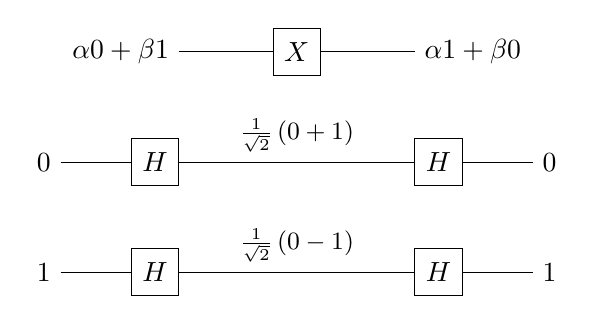
\begin{tikzpicture}[
            gate/.style={draw, fill=white, minimum size=6mm, inner sep=1pt},
        ]
        % X gate
        \draw (1.5,2.8) -- (4.5,2.8);
        \node[left] at (1.5,2.8) {$\alpha\ket{0} + \beta\ket{1}$};
        \node[gate] at (3,2.8) {$X$};
        \node[right] at (4.5,2.8) {$\alpha\ket{1} + \beta\ket{0}$};
        % H applied twice to |0> and to |1>
        \draw (0,1.4) -- (6,1.4);
        \node[left] at (0,1.4) {$\ket{0}$};
        \node[gate] at (1.2,1.4) {$H$};
        \node[above] at (3,1.4) {\small $\frac{1}{\sqrt{2}}\left(\ket{0} + \ket{1}\right)$};
        \node[gate] at (4.8,1.4) {$H$};
        \node[right] at (6,1.4) {$\ket{0}$};
        \draw (0,0) -- (6,0);
        \node[left] at (0,0) {$\ket{1}$};
        \node[gate] at (1.2,0) {$H$};
        \node[above] at (3,0) {\small $\frac{1}{\sqrt{2}}\left(\ket{0} - \ket{1}\right)$};
        \node[gate] at (4.8,0) {$H$};
        \node[right] at (6,0) {$\ket{1}$};
    \end{tikzpicture}
    \caption{One-qubit circuits. Top: the $X$ gate. Below: the Hadamard gate applied twice gives
        back the input, since $H^2 = I$ (\cref{lem:hh-0915}).}
    \label{fig:xh-0915}
\end{figure}

\section{The CNOT Gate}

\begin{definition}[CNOT Gate]\label{def:cnot-0915}
    The \textbf{controlled-NOT gate} (CNOT) is the two-qubit gate that maps the basis states by
    \[\ket{a} \ket{b} \longmapsto \ket{a} \ket{b \oplus a}, \qquad a, b \in \set{0,1},\]
    where $\oplus$ is XOR (addition modulo $2$). The first qubit $\ket{a}$ is the \textbf{control}
    qubit and is left unchanged; the second qubit $\ket{b}$ is the \textbf{target} qubit and is flipped
    exactly when $a = 1$. See \cref{fig:cnot-0915}.
\end{definition}

\begin{figure}[ht]
    \centering
    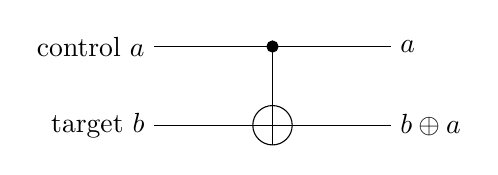
\begin{tikzpicture}
        \draw (0,1) -- (3,1);
        \draw (0,0) -- (3,0);
        \node[left] at (0,1) {control $\ket{a}$};
        \node[left] at (0,0) {target $\ket{b}$};
        \filldraw (1.5,1) circle (2pt);
        \draw (1.5,1) -- (1.5,-0.25);
        \draw (1.5,0) circle (0.25);
        \node[right] at (3,1) {$\ket{a}$};
        \node[right] at (3,0) {$\ket{b \oplus a}$};
    \end{tikzpicture}
    \caption{The CNOT gate: a filled dot on the control qubit and $\oplus$ on the target qubit.}
    \label{fig:cnot-0915}
\end{figure}

The four basis states are mapped as follows (for example $a = 1$, $b = 1$ gives $b \oplus a = 0$):
\[\begin{array}{c|cccc}
        \ket{a b}          & \ket{00} & \ket{01} & \ket{10} & \ket{11} \\ \hline
        \ket{a, b \oplus a} & \ket{00} & \ket{01} & \ket{11} & \ket{10}
    \end{array}\]

\begin{lemma}[Matrix of the CNOT Gate]\label{lem:cnot-0915}
    The matrix of the CNOT gate, with rows and columns indexed by $00, 01, 10, 11$, is the
    permutation matrix
    \[U_{\mathrm{CNOT}} = \begin{pmatrix}
            1 & 0 & 0 & 0 \\
            0 & 1 & 0 & 0 \\
            0 & 0 & 0 & 1 \\
            0 & 0 & 1 & 0
        \end{pmatrix}.\]
    It is unitary.
\end{lemma}

\begin{proof}
    The columns of the matrix of a gate are the images of the basis states. By the table, the images
    of $\ket{00}, \ket{01}, \ket{10}, \ket{11}$ are $\ket{00}, \ket{01}, \ket{11}, \ket{10}$, i.e., the
    column vectors
    \[\begin{pmatrix} 1 \\ 0 \\ 0 \\ 0 \end{pmatrix}, \quad
        \begin{pmatrix} 0 \\ 1 \\ 0 \\ 0 \end{pmatrix}, \quad
        \begin{pmatrix} 0 \\ 0 \\ 0 \\ 1 \end{pmatrix}, \quad
        \begin{pmatrix} 0 \\ 0 \\ 1 \\ 0 \end{pmatrix},\]
    which are the four columns of $U_{\mathrm{CNOT}}$, in this order.

    The map $\pi \colon (a, b) \mapsto (a, b \oplus a)$ on $\set{0,1}^2$ is its own inverse, since
    $\pi(\pi(a, b)) = (a, b \oplus a \oplus a) = (a, b)$. Hence $\pi$ is a bijection, i.e., a
    permutation of the four basis states, and $U_{\mathrm{CNOT}}$ is a \emph{permutation matrix}: every
    column is a standard basis vector, and different columns are different basis vectors.

    Every permutation matrix $P$ is unitary. The $(j, k)$ entry of $P^T P$ is the inner product of the
    $\nth{j}$ and the $\nth{k}$ column of $P$. These columns are standard basis vectors, equal if
    $j = k$ and different if $j \neq k$, so the entry is $1$ if $j = k$ and $0$ otherwise. Thus
    $P^T P = I$, and since $P$ is real, $P^\dagger P = P^T P = I$.
\end{proof}

In block form, $U_{\mathrm{CNOT}} = \begin{pmatrix} I & 0 \\ 0 & X \end{pmatrix}$: if the control is
$0$ (first two rows and columns) nothing happens, and if it is $1$ the gate $X$ is applied to the target.

\subsection{Classical Gates Are Not Reversible}

By \cref{thm:unitary-0915} and the remark after it, every quantum gate is unitary and therefore
invertible: the computation can be undone by applying $U^\dagger$. Classical gates such as AND, OR and
XOR, which take two bits to one bit, are \emph{not bijective}, hence \emph{not reversible}, hence
\emph{not unitary}. (Some classical gates, such as NOT, are reversible; the statement is about gates
that lose information.)

\begin{lemma}[XOR Is Not Reversible]\label{lem:xor-0915}
    The classical gate $\mathrm{XOR} \colon \set{0,1}^2 \to \set{0,1}$, $(a, b) \mapsto a \oplus b$, is
    not injective, so its input cannot be recovered from its output. The linear map
    $T \colon \mathbb{C}^4 \to \mathbb{C}^2$ with $T \ket{a b} = \ket{a \oplus b}$ does not preserve
    norms, so it is not unitary. The same holds for every gate with two input bits and one output bit.
\end{lemma}

\begin{proof}
    $\mathrm{XOR}(0,0) = 0 = \mathrm{XOR}(1,1)$, so two different inputs have the same output, and no
    function of the output can return the input in both cases. For the linear map,
    $T\left(\ket{00} - \ket{11}\right) = \ket{0} - \ket{0} = 0$, although
    $\norm{\ket{00} - \ket{11}} = \sqrt{2} \neq 0$. For a general gate $g \colon \set{0,1}^2 \to \set{0,1}$ there are four inputs and only two
    outputs, so by the pigeonhole principle two inputs $u \neq v$ have $g(u) = g(v)$, and the same
    argument applies with $\ket{u} - \ket{v}$. (For AND, take $u = 00$ and $v = 01$; for OR, $u = 01$
    and $v = 11$.)
\end{proof}

The CNOT gate is the reversible version of XOR: it computes $b \oplus a$ on the target wire, but it
also keeps a copy of $a$ on the control wire, and from $(a, b \oplus a)$ we recover
$b = (b \oplus a) \oplus a$. The example written in red in the notes and drawn on the board is the collision of XOR: the inputs
$00$ and $11$ give the same output $0$. In contrast, CNOT maps $\ket{00}$ to $\ket{00}$ and $\ket{11}$
to $\ket{10}$, two different outputs.

\section{Tensor Products and Entanglement}

The state of two qubits is built from the states of the single qubits by the tensor product.

\begin{definition}[Tensor Product]\label{def:tensor-0915}
    Let $A = (a_{ij})$ be an $m \times n$ matrix and let $B$ be a $p \times q$ matrix. The
    \textbf{tensor product} (Kronecker product) $A \otimes B$ is the $mp \times nq$ block matrix
    \[A \otimes B = \begin{pmatrix}
            a_{11} B & a_{12} B & \cdots & a_{1n} B \\
            a_{21} B & a_{22} B & \cdots & a_{2n} B \\
            \vdots   &          &        & \vdots   \\
            a_{m1} B & a_{m2} B & \cdots & a_{mn} B
        \end{pmatrix}.\]
    Column vectors are matrices with one column, so in particular
    \[\begin{pmatrix} \alpha \\ \beta \end{pmatrix} \otimes \begin{pmatrix} \gamma \\ \delta \end{pmatrix}
        = \begin{pmatrix} \alpha\gamma \\ \alpha\delta \\ \beta\gamma \\ \beta\delta \end{pmatrix}.\]
\end{definition}

For basis states this gives, for example,
$\ket{0} \otimes \ket{0} = (1, 0, 0, 0)^T = \ket{00}$ and
$\ket{1} \otimes \ket{0} = (0, 0, 1, 0)^T = \ket{10}$, and in general
\[\ket{a} \ket{b} = \ket{a} \otimes \ket{b} = \ket{a b}, \qquad a, b \in \set{0,1};\]
the three ways of writing are used interchangeably. In terms of kets, the formula for two vectors reads
\[\left(\alpha \ket{0} + \beta \ket{1}\right) \otimes \left(\gamma \ket{0} + \delta \ket{1}\right)
    = \alpha\gamma \ket{00} + \alpha\delta \ket{01} + \beta\gamma \ket{10} + \beta\delta \ket{11},\]
i.e., the tensor product is multiplied out like a product of sums. Gates combine in the same way: if
$A$ is applied to the first qubit and $B$ to the second, the two-qubit gate is $A \otimes B$, and
\begin{equation}\label{eq:mixed-0915}
    (A \otimes B)\left(\ket{x} \otimes \ket{y}\right) = A \ket{x} \otimes B \ket{y}.
\end{equation}
Indeed, if $x_1, \dots, x_n$ are the entries of $\ket{x}$, then $\ket{x} \otimes \ket{y}$ consists of
the blocks $x_1 \ket{y}, \dots, x_n \ket{y}$, so the $\nth{i}$ block of the left-hand side is
$\sum_{j} a_{ij} B \left(x_j \ket{y}\right) = \left(\sum_j a_{ij} x_j\right) B \ket{y}$, which is the
$\nth{i}$ block of the right-hand side.

\begin{definition}[Product State, Entangled State]
    A two-qubit state $\ket{\psi}$ is a \textbf{product state} if
    $\ket{\psi} = \ket{\phi_1} \otimes \ket{\phi_2}$ for some one-qubit states $\ket{\phi_1}$,
    $\ket{\phi_2}$. Otherwise $\ket{\psi}$ is \textbf{entangled}.
\end{definition}

In a product state each qubit has a state of its own. This is not always the case: the two qubits of
the \emph{Bell state} $\frac{1}{\sqrt{2}} \ket{00} + \frac{1}{\sqrt{2}} \ket{11}$ are entangled.

% Notes p. 10 (board): "1/sqrt2 |00> + 1/sqrt2 |11>  =/=  |alpha>|beta>", annotated "entangled
% qubits"; stated without proof.
\begin{exercise}\label{ex:bell-0915}
    Show that $\frac{1}{\sqrt{2}} \ket{00} + \frac{1}{\sqrt{2}} \ket{11} \neq \ket{\alpha} \ket{\beta}$
    for all one-qubit states $\ket{\alpha}$, $\ket{\beta}$.
\end{exercise}

The solution is \cref{thm:bell-0915}.

\begin{theorem}[The Bell State Is Entangled]\label{thm:bell-0915}
    The state $\frac{1}{\sqrt{2}} \ket{00} + \frac{1}{\sqrt{2}} \ket{11}$ is not a product state:
    there are no vectors $\ket{\phi_1}, \ket{\phi_2} \in \mathbb{C}^2$ with
    \[\frac{1}{\sqrt{2}} \ket{00} + \frac{1}{\sqrt{2}} \ket{11} = \ket{\phi_1} \otimes \ket{\phi_2}.\]
\end{theorem}

\begin{proof}
    Suppose there are, and write $\ket{\phi_1} = \begin{pmatrix} \alpha \\ \beta \end{pmatrix}$ and
    $\ket{\phi_2} = \begin{pmatrix} \gamma \\ \delta \end{pmatrix}$. By \cref{def:tensor-0915},
    comparing the four entries of the two sides gives
    \[\alpha\gamma = \frac{1}{\sqrt{2}}, \qquad \alpha\delta = 0, \qquad \beta\gamma = 0,
        \qquad \beta\delta = \frac{1}{\sqrt{2}}.\]
    From $\alpha\delta = 0$ we get $\alpha = 0$ or $\delta = 0$. If $\alpha = 0$ then
    $\alpha\gamma = 0 \neq \sfrac{1}{\sqrt{2}}$, and if $\delta = 0$ then
    $\beta\delta = 0 \neq \sfrac{1}{\sqrt{2}}$. Both cases are contradictions.
\end{proof}


\newlecture{September 17, 2026}{Linear Algebra Review: Column Space, Rank, Linear Independence,
    Orthogonality}
In this lecture, we review the linear algebra that the quantum part of the course rests on. We read
the product $Ax$ as a combination of the columns of $A$, define linear independence, the column rank
and the row rank of a matrix, and show that a nonzero vector orthogonal to a set of independent vectors
is independent of them.

\section{The Product \texorpdfstring{$Ax$}{Ax} as a Combination of Columns}

In the previous lecture we saw that $y = Ax$ is a linear combination of the columns of $A$, with the
entries of $x$ as coefficients. We work this out on the example
\[A = \begin{bmatrix} 2 & 1 & 3 \\ 3 & 1 & 4 \\ 5 & 7 & 12 \end{bmatrix} \in \mathbb{R}^{3 \times 3},
    \qquad x = \begin{bmatrix} x_1 \\ x_2 \\ x_3 \end{bmatrix},\]
whose columns we call $v_1 = (2, 3, 5)^{T}$, $v_2 = (1, 1, 7)^{T}$ and $v_3 = (3, 4, 12)^{T}$. Then
\begin{equation}\label{eq:columns-0917}
    Ax = \begin{bmatrix} 2x_1 + x_2 + 3x_3 \\ 3x_1 + x_2 + 4x_3 \\ 5x_1 + 7x_2 + 12x_3 \end{bmatrix}
    = x_1 \begin{bmatrix} 2 \\ 3 \\ 5 \end{bmatrix} + x_2 \begin{bmatrix} 1 \\ 1 \\ 7 \end{bmatrix}
    + x_3 \begin{bmatrix} 3 \\ 4 \\ 12 \end{bmatrix}
    = x_1 v_1 + x_2 v_2 + x_3 v_3.
\end{equation}
In this example the third column is the sum of the first two, $v_3 = v_1 + v_2$, because
$2 + 1 = 3$, $3 + 1 = 4$ and $5 + 7 = 12$. Substituting this into \cref{eq:columns-0917} gives
\begin{equation}\label{eq:twocolumns-0917}
    Ax = x_1 v_1 + x_2 v_2 + x_3 (v_1 + v_2) = (x_1 + x_3)\, v_1 + (x_2 + x_3)\, v_2,
\end{equation}
so every output $Ax$ is already a combination of $v_1$ and $v_2$ alone.

The matrix $A$ defines a linear map $T \colon \mathbb{R}^3 \to \mathbb{R}^3$, $T(x) = Ax$. In general, an
$m \times n$ matrix $A$ with columns $a_1, \dots, a_n$ defines the linear map
$T \colon \mathbb{R}^n \to \mathbb{R}^m$, $T(x) = Ax = x_1 a_1 + \dots + x_n a_n$, and its \emph{image}
is the set of all outputs,
\[\operatorname{Im}(A) = \set{Ax \given x \in \mathbb{R}^n} = \operatorname{span}(a_1, \dots, a_n).\]
The second equality is exactly the statement that $Ax$ is a combination of the columns: the image of
$A$ is its \emph{column space}.

\section{Linear Independence and Rank}

\begin{definition}[Linear Independence]
    Vectors $v_1, \dots, v_k$ are \textbf{linearly independent} if
    \[c_1 v_1 + c_2 v_2 + \dots + c_k v_k = 0 \quad\Longrightarrow\quad c_1 = c_2 = \dots = c_k = 0,\]
    i.e., the only combination of them that gives the zero vector is the trivial one. Otherwise they are
    \textbf{linearly dependent}. If $v_1, \dots, v_k$ are linearly independent, we say that a vector $v$
    is \emph{independent of} them if $v, v_1, \dots, v_k$ are linearly independent.
\end{definition}

\begin{definition}[Column Rank and Row Rank]
    The \textbf{column rank} $\operatorname{rank}_c(A)$ of a matrix $A$ is the maximum number of linearly
    independent columns of $A$. The \textbf{row rank} $\operatorname{rank}_r(A)$ is the maximum number of
    linearly independent rows of $A$.
\end{definition}

We use one fact about a subspace $W$ spanned by $r$ vectors $z_1, \dots, z_r$: any $r + 1$ vectors
$y_1, \dots, y_{r+1}$ of $W$ are linearly dependent. Indeed, write $y_j = \sum_{l=1}^{r} t_{lj} z_l$. The
homogeneous system $\sum_{j=1}^{r+1} t_{lj} c_j = 0$ ($1 \leq l \leq r$) has $r$ equations in $r + 1$
unknowns, so it has a solution $(c_1, \dots, c_{r+1}) \neq 0$ (see below), and then
$\sum_{j} c_j y_j = \sum_{l} \big(\sum_{j} t_{lj} c_j\big) z_l = 0$. Hence two bases of $W$ cannot have
different sizes (the larger one would consist of more vectors than span $W$, and so be dependent); the
common size is the \emph{dimension} $\dim(W)$.

That a homogeneous system of $r$ linear equations in more than $r$ unknowns has a nonzero solution
follows by induction on $r$. For $r = 0$ there are no equations and any nonzero vector is a solution.
For $r \geq 1$, if no equation contains $c_1$, set $c_1 = 1$ and all other unknowns to $0$. Otherwise
solve one equation that contains $c_1$ for $c_1$ and substitute into the others: this leaves $r - 1$
equations in the remaining unknowns, of which there are more than $r - 1$, so by induction they have a
nonzero solution, and the solved equation then gives the value of $c_1$. The column rank is the dimension of the image:

\begin{lemma}[Column Rank Is the Dimension of the Image]\label{lem:colbasis-0917}
    Let $A$ be an $m \times n$ matrix with $r = \operatorname{rank}_c(A) \geq 1$. Then any $r$ linearly
    independent columns of $A$ form a basis of $\operatorname{Im}(A)$. In particular,
    \[\operatorname{rank}_c(A) = \dim(\operatorname{Im}(A)).\]
\end{lemma}

\begin{proof}
    Let $w_1, \dots, w_r$ be independent columns of $A$ and let $a$ be any column of $A$. By the
    definition of $r$, the vectors $a, w_1, \dots, w_r$ are dependent (trivially so if $a$ is one of the
    $w_l$): $\beta a + \beta_1 w_1 + \dots + \beta_r w_r = 0$ with coefficients that are not all zero.
    Here $\beta \neq 0$, since otherwise this would be a nontrivial relation among $w_1, \dots, w_r$.
    Hence $a = -\frac{1}{\beta}(\beta_1 w_1 + \dots + \beta_r w_r) \in \operatorname{span}(w_1, \dots, w_r)$.
    So every column of $A$, and therefore every combination of columns, lies in
    $\operatorname{span}(w_1, \dots, w_r)$: the independent vectors $w_1, \dots, w_r$ span
    $\operatorname{Im}(A)$ and form a basis of it.
\end{proof}

% Not marked on the board; stated without proof. Page 1, rows 2-4: "# ind cols = rank_c(A) =
% dim(Im(A))", "# ind rows rank_r(A)", "[1 0 1], [0 1 1], [2 1 3] = 2[1 0 1] + 1[0 1 1]".
\begin{exercise}\label{ex:example-rank-0917}
    For the matrix $A$ of \cref{eq:columns-0917}, find $\operatorname{rank}_c(A)$,
    $\operatorname{Im}(A)$ and $\operatorname{rank}_r(A)$, and express every row of $A$ as a combination
    of $[1\ 0\ 1]$ and $[0\ 1\ 1]$.
\end{exercise}

\begin{wsolution}
    \emph{Columns.} The columns $v_1, v_2$ are independent: $a v_1 + b v_2 = 0$ reads $2a + b = 0$,
    $3a + b = 0$, $5a + 7b = 0$; subtracting the first equation from the second gives $a = 0$, and then
    $b = 0$. All three columns are dependent, since $v_1 + v_2 - v_3 = 0$. Hence
    $\operatorname{rank}_c(A) = 2$, and by \cref{lem:colbasis-0917},
    \[\operatorname{Im}(A) = \operatorname{span}(v_1, v_2), \qquad \dim(\operatorname{Im}(A)) = 2.\]

    \emph{Rows.} Let $u_1 = [1\ 0\ 1]$ and $u_2 = [0\ 1\ 1]$, so that $a u_1 + b u_2 = [a\ \ b\ \ a + b]$.
    Then
    \[[2\ 1\ 3] = 2 u_1 + 1 u_2, \qquad [3\ 1\ 4] = 3 u_1 + 1 u_2, \qquad [5\ 7\ 12] = 5 u_1 + 7 u_2.\]
    So all three rows lie in $\operatorname{span}(u_1, u_2)$, and any three vectors in the span of two
    vectors are dependent: $\operatorname{rank}_r(A) \leq 2$. The first
    two rows are independent: $a\,[2\ 1\ 3] + b\,[3\ 1\ 4] = 0$ gives $a + b = 0$ from the second entry
    and $2a + 3b = 0$ from the first, so $b = 0$ and $a = 0$. Hence $\operatorname{rank}_r(A) = 2$.
\end{wsolution}

In the example the two ranks agree. This is not a coincidence.

% Not marked on the board; stated without proof. Page 1, rows 2-3: both rank_c(A) and rank_r(A) are
% defined for the same matrix and computed to be equal in the example.
\begin{exercise}\label{ex:rank-equal-0917}
    Show that $\operatorname{rank}_r(A) = \operatorname{rank}_c(A)$ for every matrix $A$.
\end{exercise}

The solution is \cref{thm:rank-equal-0917}.

\begin{theorem}[Row Rank Equals Column Rank]\label{thm:rank-equal-0917}
    For every $m \times n$ matrix $A$, $\operatorname{rank}_r(A) = \operatorname{rank}_c(A)$. This common
    value is called the \textbf{rank} of $A$.
\end{theorem}

\begin{proof}
    We first show $\operatorname{rank}_r(A) \leq \operatorname{rank}_c(A)$. Let
    $r = \operatorname{rank}_c(A)$. If $r = 0$, then every column of $A$ is zero (a single nonzero vector
    is independent), so $A = 0$ and $\operatorname{rank}_r(A) = 0$ as well. Let $r \geq 1$, and let
    $w_1, \dots, w_r$ be independent columns of $A$; write $w_{il}$ for the $\nth{i}$ entry of $w_l$, so
    that $W = (w_{il})$ is the $m \times r$ matrix with columns $w_1, \dots, w_r$. By
    \cref{lem:colbasis-0917}, every column $a_j$ of $A$ is a combination of them: there are numbers
    $s_{lj}$ with
    \[a_j = \sum_{l=1}^{r} s_{lj} \, w_l \qquad (1 \leq j \leq n).\]
    Let $S = (s_{lj})$, an $r \times n$ matrix with rows $\rho_1, \dots, \rho_r$. Taking the $\nth{i}$
    entry on both sides, the entries of $A$ are $a_{ij} = \sum_{l=1}^{r} w_{il} \, s_{lj}$, that is,
    $A = WS$. Now fix $i$ and let $j$ run from $1$ to $n$: the same equation says that
    \[\text{row $i$ of $A$} \;=\; \sum_{l=1}^{r} w_{il} \, \rho_l.\]
    So every row of $A$ lies in $\operatorname{span}(\rho_1, \dots, \rho_r)$. Any $r + 1$ vectors in the
    span of $r$ vectors are dependent, so $A$ has at most $r$ independent rows:
    $\operatorname{rank}_r(A) \leq r = \operatorname{rank}_c(A)$.

    This holds for every matrix, in particular for the transpose $A^{T}$, whose rows are the columns of
    $A$ and whose columns are the rows of $A$. Hence
    \[\operatorname{rank}_c(A) = \operatorname{rank}_r(A^{T}) \leq \operatorname{rank}_c(A^{T})
        = \operatorname{rank}_r(A),\]
    and the two inequalities together give $\operatorname{rank}_r(A) = \operatorname{rank}_c(A)$.
\end{proof}

For the example, with $w_1 = v_1$ and $w_2 = v_2$, the rows of $S$ are exactly the two row vectors
$[1\ 0\ 1]$ and $[0\ 1\ 1]$ from above.

\section{Orthogonality}

The results of this section hold over $\mathbb{R}$ and over $\mathbb{C}$.
For $a, b \in \mathbb{R}^n$ the inner product is $\langle a, b \rangle = a \cdot b = \sum_{i=1}^{n} a_i b_i$.
For $a, b \in \mathbb{C}^n$ it is $\langle a, b \rangle = \sum_{i=1}^{n} \overline{a_i} \, b_i$, which is
linear in $b$. In both cases $\langle a, a \rangle = \sum_{i=1}^{n} \abs{a_i}^2 = \norm{a}^2$, which is
$0$ only for $a = 0$.

\begin{definition}[Orthogonality]
    Two vectors $a$ and $b$ are \textbf{orthogonal} if $\langle a, b \rangle = 0$; for real vectors,
    $a \cdot b = 0$.
\end{definition}

% Not marked on the board; stated without proof. Page 1, rows 5-7: "v is orthogonal to v_1, v_2, ...,
% v_k (ind vectors) then v is ind of v_1, v_2, ..., v_k", followed only by the definition of independence.
\needspace{12\baselineskip} % keep the exercise and the start of its solution on one page
\begin{exercise}\label{ex:orth-ind-0917}
    Let $v_1, \dots, v_k$ be linearly independent vectors. Show that if a nonzero vector $v$ is
    orthogonal to $v_1, v_2, \dots, v_k$, then $v$ is independent of $v_1, v_2, \dots, v_k$.
\end{exercise}

The solution is \cref{thm:orth-ind-0917}; the other reading of the line on the board is
\cref{cor:pairwise-orth-0917}.

\begin{theorem}[Orthogonal Implies Independent]\label{thm:orth-ind-0917}
    Let $v_1, \dots, v_k$ be linearly independent vectors in $\mathbb{R}^n$ or $\mathbb{C}^n$, and let
    $v \neq 0$ be orthogonal to each of them. Then $v, v_1, \dots, v_k$ are linearly independent. In
    particular, $v \notin \operatorname{span}(v_1, \dots, v_k)$.
\end{theorem}

\begin{proof}
    Suppose that $c \, v + c_1 v_1 + \dots + c_k v_k = 0$. Taking the inner product of $v$ with both
    sides, and using linearity in the second argument and $\langle v, v_i \rangle = 0$ for all $i$,
    \[0 = \langle v, \; c \, v + c_1 v_1 + \dots + c_k v_k \rangle
        = c \, \langle v, v \rangle + \sum_{i=1}^{k} c_i \, \langle v, v_i \rangle
        = c \, \norm{v}^2.\]
    Since $v \neq 0$, we have $\norm{v}^2 > 0$, so $c = 0$. The relation becomes
    $c_1 v_1 + \dots + c_k v_k = 0$, and the independence of $v_1, \dots, v_k$ gives
    $c_1 = \dots = c_k = 0$. So all coefficients vanish and $v, v_1, \dots, v_k$ are independent. If we
    had $v = \sum_{i} \alpha_i v_i$, then $1 \cdot v - \sum_{i} \alpha_i v_i = 0$ would be a nontrivial
    relation, so $v \notin \operatorname{span}(v_1, \dots, v_k)$.
\end{proof}

\paragraph{Remark.} The assumption $v \neq 0$ is needed: the zero vector is orthogonal to every vector,
but no set of vectors that contains it is independent ($1 \cdot 0 = 0$ is a nontrivial relation).

If $v_1, \dots, v_k$ are instead only assumed to be nonzero and pairwise orthogonal, then the implication
$c_1 v_1 + \dots + c_k v_k = 0 \Rightarrow c_1 = \dots = c_k = 0$ becomes the conclusion:

\begin{corollary}[Orthogonal Vectors are Independent]\label{cor:pairwise-orth-0917}
    Let $v_1, \dots, v_k$ be nonzero vectors that are pairwise orthogonal, i.e.,
    $\langle v_i, v_j \rangle = 0$ for all $i \neq j$. Then $v_1, \dots, v_k$ are linearly independent.
\end{corollary}

\begin{proof}
    Suppose that $c_1 v_1 + \dots + c_k v_k = 0$ and fix $j$. Taking the inner product of $v_j$ with
    both sides, all terms with $i \neq j$ vanish, and
    \[0 = \sum_{i=1}^{k} c_i \, \langle v_j, v_i \rangle = c_j \, \norm{v_j}^2.\]
    Since $v_j \neq 0$, this gives $c_j = 0$. This holds for every $j$, so the vectors are independent.
\end{proof}

In particular, the vectors of an orthonormal set, such as the basis states of a quantum system, are
always linearly independent, and $n$ of them in an $n$-dimensional space form a basis.


% TODO: September 22, 2026 (quantum circuits) -- no handwritten pages exported yet.

\newlecture{September 24, 2026}{Deutsch's Algorithm, Phase Flip, Walsh--Hadamard Transform,
    Deutsch--Jozsa Algorithm}
In this lecture, we see the first quantum algorithms that beat every classical algorithm in the
query model: Deutsch's algorithm and, using the \emph{phase flip} form of a query and the $n$-qubit
Hadamard (Walsh--Hadamard) transform, the Deutsch--Jozsa algorithm.

\section{Deutsch's Algorithm}

\begin{problem}[Deutsch's Problem]
    Given a function $f \colon \set{0,1} \to \set{0,1}$ as a black box, determine whether $f$ is
    \emph{constant} ($f(0) = f(1)$) or \emph{balanced} ($f(0) \neq f(1)$).
\end{problem}

Classically we need $2$ queries: after one query, say $f(0)$, both answers are still possible.
Quantumly, Deutsch's algorithm does it with $1$ query.

\subsection{The Quantum Query \texorpdfstring{$U_f$}{Uf}}

A quantum circuit is reversible, but $f$ need not be. We therefore convert $f$ into a reversible
\emph{quantum version} $U_f$, a controlled-$f$ gate like the CNOT gate of \cref{def:cnot-0915}
(\cref{fig:uf-0924}):
\[U_f \colon \ket{a}\ket{b} \longmapsto \ket{a}\ket{b \oplus f(a)}.\]
Applying $U_f$ twice gives back $\ket{a}\ket{b}$, so $U_f$ is reversible. One application of $U_f$
counts as one query to $f$.

\begin{figure}[ht]
    \centering
    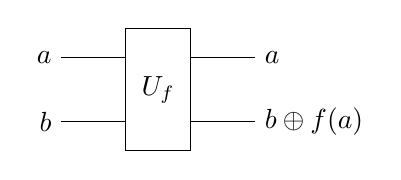
\begin{tikzpicture}[scale=0.82]
        \draw (0,1) -- (3,1);
        \draw (0,0) -- (3,0);
        \node[left] at (0,1) {$\ket{a}$};
        \node[left] at (0,0) {$\ket{b}$};
        \draw[fill=white] (1,-0.45) rectangle (2,1.45);
        \node at (1.5,0.5) {$U_f$};
        \node[right] at (3,1) {$\ket{a}$};
        \node[right] at (3,0) {$\ket{b \oplus f(a)}$};
    \end{tikzpicture}
    \caption{The quantum query $U_f$.}
    \label{fig:uf-0924}
\end{figure}

\subsection{The Circuit}

In Deutsch's algorithm (\cref{fig:deutsch-0924}) the qubits start in $\ket{0}$ and $\ket{1}$, go
through a Hadamard gate each, then through $U_f$, then through a Hadamard gate each, and are measured.

\begin{figure}[ht]
    \centering
    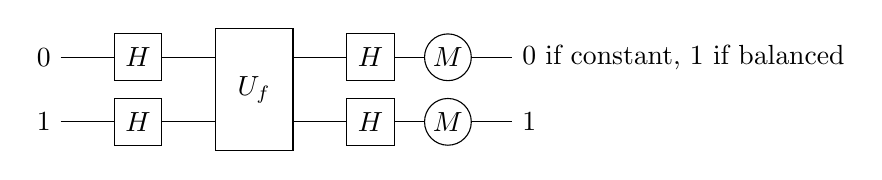
\begin{tikzpicture}[scale=0.82, 
            gate/.style={draw, fill=white, minimum size=6mm, inner sep=1pt},
            meter/.style={draw, circle, fill=white, inner sep=1.5pt},
        ]
        % wires
        \draw (0,1) -- (7,1);
        \draw (0,0) -- (7,0);
        \node[left] at (0,1) {$\ket{0}$};
        \node[left] at (0,0) {$\ket{1}$};
        % query
        \draw[fill=white] (2.4,-0.45) rectangle (3.6,1.45);
        \node at (3,0.5) {$U_f$};
        % Hadamard gates and measurements
        \foreach \y in {0,1} {
                \node[gate] at (1.2,\y) {$H$};
                \node[gate] at (4.8,\y) {$H$};
                \node[meter] at (6,\y) {$M$};
            }
        \node[right] at (7,1) {$\ket{0}$ if constant, $\ket{1}$ if balanced};
        \node[right] at (7,0) {$\ket{1}$};
    \end{tikzpicture}
    \caption{Deutsch's algorithm.}
    \label{fig:deutsch-0924}
\end{figure}

By \cref{eq:hadamard-0915}, for $a \in \set{0,1}$,
\begin{equation}\label{eq:hadamard-0924}
    H\ket{a} = \frac{1}{\sqrt{2}}\left(\ket{0} + (-1)^{a}\ket{1}\right)
    = \frac{1}{\sqrt{2}} \sum_{b \in \set{0,1}} (-1)^{ab} \ket{b}.
\end{equation}

\begin{exercise}\label{ex:hback-0924}
    Compute $H \, \frac{1}{\sqrt{2}}\left(\ket{0} + (-1)^{a}\ket{1}\right)$ for $a \in \set{0,1}$.
\end{exercise}

\begin{wsolution}
    By linearity and \cref{eq:hadamard-0924} for $H\ket{0}$ and $H\ket{1}$,
    \[H \, \tfrac{1}{\sqrt{2}}\left(\ket{0} + (-1)^{a}\ket{1}\right)
        = \tfrac{1}{2}\left(\ket{0} + \ket{1}\right) + \tfrac{(-1)^{a}}{2}\left(\ket{0} - \ket{1}\right)
        = \tfrac{1 + (-1)^{a}}{2}\ket{0} + \tfrac{1 - (-1)^{a}}{2}\ket{1}.\]
    For $a = 0$ this is $\ket{0}$ and for $a = 1$ it is $\ket{1}$, so the result is $\ket{a}$. This
    agrees with $H^2 = I$ (\cref{lem:hh-0915}).
\end{wsolution}

\begin{exercise}\label{ex:deutsch-0924}
    In the circuit of \cref{fig:deutsch-0924} the second qubit is measured as $\ket{1}$. What does the
    measurement of the first qubit give?
\end{exercise}

The answer is $\ket{0}$ if $f$ is constant and $\ket{1}$ if $f$ is balanced:

\begin{theorem}[Deutsch's Algorithm]\label{thm:deutsch-0924}
    The circuit of \cref{fig:deutsch-0924} makes one query to $f$, and measuring its first qubit gives
    $f(0) \oplus f(1)$ with probability $1$. Hence the outcome is $0$ if $f$ is constant and $1$ if $f$
    is balanced.
\end{theorem}

\begin{proof}
    After the first two Hadamard gates the state is (by \cref{eq:mixed-0915})
    $\ket{\psi_1} = H\ket{0} \otimes H\ket{1}
        = \frac{1}{2}\left(\ket{0} + \ket{1}\right)\left(\ket{0} - \ket{1}\right)$.
    For $c \in \set{0,1}$ we have
    $\ket{0 \oplus c} - \ket{1 \oplus c} = (-1)^{c}\left(\ket{0} - \ket{1}\right)$ (for $c = 1$ the two
    kets are swapped), so $U_f$ maps $\ket{a}\left(\ket{0} - \ket{1}\right)$ to
    $(-1)^{f(a)} \ket{a}\left(\ket{0} - \ket{1}\right)$ and, by linearity,
    \[\ket{\psi_2} = U_f \ket{\psi_1}
        = \frac{1}{\sqrt{2}}\left((-1)^{f(0)}\ket{0} + (-1)^{f(1)}\ket{1}\right)
        \otimes \frac{1}{\sqrt{2}}\left(\ket{0} - \ket{1}\right).\]
    Since $(-1)^{f(1)} = (-1)^{f(0)} (-1)^{f(0) \oplus f(1)}$, the first qubit is
    $(-1)^{f(0)} \frac{1}{\sqrt{2}}\left(\ket{0} + (-1)^{f(0) \oplus f(1)}\ket{1}\right)$, i.e., up to the
    sign $(-1)^{f(0)}$, the state of \cref{ex:hback-0924} with $a = f(0) \oplus f(1)$; the
    second qubit is $H\ket{1}$. So the last two Hadamard gates give
    $\ket{\psi_3} = (-1)^{f(0)} \ket{f(0) \oplus f(1)} \ket{1}$.
    The global phase $(-1)^{f(0)}$ does not affect the measurement: the first qubit gives
    $f(0) \oplus f(1)$ with probability $1$, and the second always gives $1$.
\end{proof}

\section{Phase Flip and the \texorpdfstring{$n$}{n}-Qubit Hadamard Transform}

If the second (target) qubit of $U_f$ is in the state
$\frac{1}{\sqrt{2}}\left(\ket{0} - \ket{1}\right)$, then, by the computation in the proof of
\cref{thm:deutsch-0924}, for every input $x$ (also for $x \in \set{0,1}^n$, where
$U_f \colon \ket{x}\ket{b} \mapsto \ket{x}\ket{b \oplus f(x)}$),
\[U_f \, \ket{x} \tfrac{1}{\sqrt{2}}(\ket{0} - \ket{1}) = (-1)^{f(x)} \, \ket{x} \tfrac{1}{\sqrt{2}}(\ket{0} - \ket{1}).\]
We drop the target qubit and write the query in the \emph{phase flip} form
\[U_f \colon \ket{x} \longmapsto (-1)^{f(x)} \ket{x}.\]
By linearity, $U_f$ maps $\sum_x \alpha_x \ket{x}$ to $\sum_x \alpha_x (-1)^{f(x)} \ket{x}$: one query
flips the sign of every $\ket{x}$ with $f(x) = 1$.

\subsection{The \texorpdfstring{$n$}{n}-Qubit Hadamard Transform}

To generalize Deutsch's algorithm to $n$ bits we apply the Hadamard gate to each of $n$ qubits.
Start with $n = 2$ and let $\ket{x} = \ket{x_1 x_2} = \ket{x_1}\ket{x_2}$. Using
\cref{eq:mixed-0915} and then \cref{eq:hadamard-0924} on each qubit,
\begin{align*}
    (H \otimes H)\ket{x}
     & = H\ket{x_1} \otimes H\ket{x_2}
    = \left(\frac{1}{\sqrt{2}} \sum_{y_1 \in \set{0,1}} (-1)^{x_1 y_1} \ket{y_1}\right)
    \left(\frac{1}{\sqrt{2}} \sum_{y_2 \in \set{0,1}} (-1)^{x_2 y_2} \ket{y_2}\right) \\
     & = \frac{1}{2} \sum_{y \in \set{0,1}^2} (-1)^{x_1 y_1 + x_2 y_2} \ket{y}
    = \frac{1}{2} \sum_{y \in \set{0,1}^2} (-1)^{x \cdot y} \ket{y},
\end{align*}
where $x \cdot y = x_1 y_1 \oplus x_2 y_2$, since only the parity of the exponent matters. For
example, $(H \otimes H)\ket{01} = \frac{1}{2}\left(\ket{00} - \ket{01} + \ket{10} - \ket{11}\right)$.
In general, for $x, y \in \set{0,1}^n$, the inner product of the bit strings modulo $2$ is
\[x \cdot y = x_1 y_1 \oplus x_2 y_2 \oplus \dots \oplus x_n y_n.\]

\begin{lemma}[Walsh--Hadamard Transform]\label{lem:wh-0924}
    The $n$-qubit Hadamard transform $H^{\otimes n} = H \otimes H \otimes \dots \otimes H$ (the
    \emph{Walsh--Hadamard transform}) acts on a basis state $\ket{x} = \ket{x_1 x_2 \cdots x_n}$ as
    \[H^{\otimes n} \ket{x} = \frac{1}{\sqrt{2^n}} \sum_{y \in \set{0,1}^n} (-1)^{x \cdot y} \ket{y}.\]
\end{lemma}

\begin{proof}
    By \cref{eq:mixed-0915} applied repeatedly, $H^{\otimes n} \ket{x} = H\ket{x_1} \otimes \dots \otimes H\ket{x_n}$,
    and by \cref{eq:hadamard-0924} the $\nth{i}$ factor is
    $\frac{1}{\sqrt{2}} \sum_{y_i \in \set{0,1}} (-1)^{x_i y_i} \ket{y_i}$. Multiplying out the $n$ sums,
    \[H^{\otimes n} \ket{x}
        = \frac{1}{\sqrt{2^n}} \sum_{y \in \set{0,1}^n} (-1)^{x_1 y_1 + \dots + x_n y_n} \ket{y},\]
    and $(-1)$ to the power $x_1 y_1 + \dots + x_n y_n$ only depends on its parity $x \cdot y$.
\end{proof}

For $x = 0^n = 00 \cdots 0$ we have $x \cdot y = 0$ for every $y$, so
$H^{\otimes n} \ket{00 \cdots 0} = \frac{1}{\sqrt{2^n}} \sum_{x \in \set{0,1}^n} \ket{x}$
is the uniform superposition of all $2^n$ bit strings.

\section{Deutsch--Jozsa Algorithm}

\begin{problem}[Deutsch--Jozsa Problem]
    Given $f \colon \set{0,1}^n \to \set{0,1}$ as a black box, with the \emph{promise} that $f$ is
    either constant or balanced (i.e., $f(x) = 0$ for exactly half of the $2^n$ inputs), determine
    which is the case.
\end{problem}

This is Deutsch's problem on $n$ bits. It is a \emph{promise problem}: we are told in advance that $f$
is one of the two kinds. Let $N = 2^n$ be the number of inputs.

\subsection{Classical Query Complexity}

\emph{Deterministic:} in the worst case $2^{n-1} + 1 = N/2 + 1$ queries are needed, since after $N/2$
equal values $f$ may still be either constant or balanced. The same holds for a randomized algorithm
that has to succeed with probability $1$.

\emph{Randomized (Monte Carlo):} query $f$ on $\alpha$ independent uniformly random inputs and output
``balanced'' if two answers differ, ``constant'' otherwise. If $f$ is constant, we are always right. If
$f$ is balanced, every answer is $0$ or $1$ with probability $\sfrac{1}{2}$ each, so all $\alpha$
answers agree, and we fail, with probability
$2 \cdot (\sfrac{1}{2})^{\alpha} = (\sfrac{1}{2})^{\alpha - 1}$. A constant number of queries gives a
constant error probability, and $\alpha = \bigO{\log N}$ queries give error probability $\sfrac{1}{N}$.

\emph{Quantum:} the Deutsch--Jozsa algorithm needs $1$ query (and $n$ measurements) and makes no error.

\subsection{The Algorithm}

The circuit (\cref{fig:dj-0924}) is Deutsch's circuit with $n$ input qubits: $n$ qubits in $\ket{0}$
and one qubit in $\ket{1}$ go through Hadamard gates and then $U_f$ (one query); then all the
qubits go through Hadamard gates again and are measured.

\begin{figure}[ht]
    \centering
    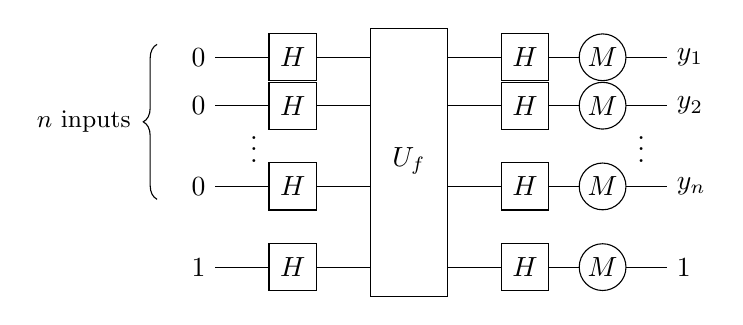
\begin{tikzpicture}[scale=0.82, 
            gate/.style={draw, fill=white, minimum size=6mm, inner sep=1pt},
            meter/.style={draw, circle, fill=white, inner sep=1.5pt},
        ]
        % wires: inputs y_1, y_2, ..., y_n, then the extra qubit
        \foreach \y in {3,2.25,1,-0.25} {\draw (0,\y) -- (7,\y);}
        \foreach \y in {3,2.25,1} {\node[left] at (0,\y) {$\ket{0}$};}
        \node[left] at (0,-0.25) {$\ket{1}$};
        \node at (0.6,1.7) {$\vdots$};
        \node at (6.6,1.7) {$\vdots$};
        % query
        \draw[fill=white] (2.4,-0.7) rectangle (3.6,3.45);
        \node at (3,1.4) {$U_f$};
        % Hadamard gates
        \foreach \y in {3,2.25,1,-0.25} {
                \node[gate] at (1.2,\y) {$H$};
                \node[gate] at (4.8,\y) {$H$};
                \node[meter] at (6,\y) {$M$};
            }
        % outputs
        \node[right] at (7,3) {$y_1$};
        \node[right] at (7,2.25) {$y_2$};
        \node[right] at (7,1) {$y_n$};
        \node[right] at (7,-0.25) {$\ket{1}$};
        % the n input qubits
        \draw[decorate, decoration={brace, amplitude=5pt}] (-0.9,0.8) -- (-0.9,3.2)
        node[midway, left=6pt] {\small $n$ inputs};
    \end{tikzpicture}
    \caption{The Deutsch--Jozsa algorithm. The last qubit always gives $1$.}
    \label{fig:dj-0924}
\end{figure}

\begin{exercise}\label{ex:dj-0924}
    The state of the $n$ input qubits before the measurement is
    $\frac{1}{2^n} \sum_{y} \sum_{x} (-1)^{f(x) + x \cdot y} \ket{y}$. What do the measurements give if
    $f$ is constant, and what if $f$ is balanced?
\end{exercise}

\begin{theorem}[Deutsch--Jozsa Algorithm]\label{thm:dj-0924}
    In the circuit of \cref{fig:dj-0924}, measuring the $n$ input qubits gives $y = 0^n$ with
    probability $1$ if $f$ is constant, and with probability $0$ if $f$ is balanced. Hence, if any
    of these $n$ measurements gives $1$, then $f$ is balanced; otherwise $f$ is constant.
\end{theorem}

\begin{proof}
    We use the phase flip form of $U_f$: the last qubit is
    $\frac{1}{\sqrt{2}}(\ket{0} - \ket{1}) = H\ket{1}$ before and after the query, so its second
    Hadamard gate gives $\ket{1}$, and we drop it. The first layer of Hadamard gates maps the input register
    $\ket{00 \cdots 0}$ to $\frac{1}{\sqrt{2^n}} \sum_{x} \ket{x}$, and the query flips the sign of
    every $\ket{x}$ with $f(x) = 1$. After the second layer of Hadamard gates, by \cref{lem:wh-0924},
    the state is
    \[\frac{1}{\sqrt{2^n}} \sum_{x \in \set{0,1}^n} (-1)^{f(x)} H^{\otimes n} \ket{x}
        = \frac{1}{2^n} \sum_{y \in \set{0,1}^n} \sum_{x \in \set{0,1}^n} (-1)^{f(x) + x \cdot y} \ket{y}.\]
    Since $x \cdot 0^n = 0$ for every $x$, the amplitude of $\ket{0^n}$ is
    $\frac{1}{2^n} \sum_{x} (-1)^{f(x)}$. If $f$ is constant, all $2^n$ terms are equal and the
    amplitude is $\pm 1$; the amplitudes squared sum to $1$, so all others are $0$ and the measurement
    gives $0^n$ with probability $1$. If $f$ is balanced, half the terms are $+1$ and half are $-1$, so
    the amplitude is $0$: the measurement gives $0^n$ with probability $0$, i.e., at least one of the
    $n$ measurements gives $1$.
\end{proof}


\newlecture{September 29, 2026}{Walsh--Hadamard Transform Recap, Bernstein--Vazirani Algorithm,
    Simon's Algorithm}
In this lecture, we see two more problems that a quantum algorithm solves with far fewer queries than
any classical algorithm: the \emph{Bernstein--Vazirani} problem and \emph{Simon's problem}, the first
exponential quantum speed-up.

\paragraph{Recap: quantum queries and the Walsh--Hadamard transform.}

Both algorithms use the query
$U_f \colon \ket{x}\ket{b} \mapsto \ket{x}\ket{b \oplus f(x)}$ (\cref{fig:uf-0924}; one application is
one query) and the \emph{Walsh--Hadamard transform} (\cref{lem:wh-0924})
$H^{\otimes n} \ket{x} = \frac{1}{\sqrt{2^n}} \sum_{y \in \set{0,1}^n} (-1)^{x \cdot y} \ket{y}$, where
$x \cdot y = x_1 y_1 \oplus \dots \oplus x_n y_n$.

\begin{lemma}[Sum of Signs]\label{lem:signsum-0929}
    For every $z \in \set{0,1}^n$,
    \[\sum_{x \in \set{0,1}^n} (-1)^{z \cdot x} =
        \begin{cases}
            2^n & \text{if } z = 0^n, \\
            0   & \text{if } z \neq 0^n.
        \end{cases}\]
\end{lemma}

\begin{proof}
    If $z = 0^n$, all $2^n$ terms are $1$. If $z \neq 0^n$, pick $i$ with $z_i = 1$ and let $e_i$ be
    the string with a single $1$ in position $i$. The map $x \mapsto x \oplus e_i$ is its own inverse
    and has no fixed point, so it splits $\set{0,1}^n$ into $2^{n-1}$ disjoint pairs
    $\set{x, x \oplus e_i}$. The inner product is linear modulo $2$, so
    $z \cdot (x \oplus e_i) = z \cdot x \oplus z_i = z \cdot x \oplus 1$, and every pair contributes
    $(-1)^{z \cdot x} + (-1)^{z \cdot x \oplus 1} = 0$.
\end{proof}

In the Deutsch--Jozsa circuit (\cref{fig:dj-0924}, \cref{thm:dj-0924}) the query acts as the phase
flip $\ket{k} \mapsto (-1)^{f(k)} \ket{k}$, and the control register after the second layer of Hadamard
gates is in the state
\begin{equation}\label{eq:dj-state-0929}
    \sum_{y \in \set{0,1}^n} \alpha_y \ket{y},
    \qquad
    \alpha_y = \frac{1}{2^n} \sum_{k \in \set{0,1}^n} (-1)^{f(k) + k \cdot y}.
\end{equation}

\section{Bernstein--Vazirani Algorithm}

\begin{problem}[Bernstein--Vazirani Problem]
    Given $f \colon \set{0,1}^n \to \set{0,1}$ as a black box, with the \emph{promise} that
    \[f(x) = s \cdot x = s_1 x_1 \oplus s_2 x_2 \oplus \dots \oplus s_n x_n\]
    for some unknown $n$-bit string $s$, find $s$.
\end{problem}

\subsection{The Algorithm}

\begin{theorem}[Bernstein--Vazirani Algorithm]\label{thm:bv-0929}
    Run the Deutsch--Jozsa circuit (\cref{fig:dj-0924}) on $f(x) = s \cdot x$. Then measuring the $n$
    control qubits gives $y = s$ with probability $1$. So a single query finds $s$.
\end{theorem}

\begin{proof}
    By \cref{eq:dj-state-0929} (with the summation index $k$ renamed $x$), the control register is in
    the state $\sum_{y} \alpha_y \ket{y}$ with
    \[\alpha_y = \frac{1}{2^n} \sum_{x \in \set{0,1}^n} (-1)^{s \cdot x \oplus y \cdot x}
        = \frac{1}{2^n} \sum_{x \in \set{0,1}^n} (-1)^{(s \oplus y) \cdot x},\]
    because only the parity of the exponent matters and the inner product is bilinear modulo $2$. By
    \cref{lem:signsum-0929} with $z = s \oplus y$, $\alpha_y = 1$ if $y = s$ and $\alpha_y = 0$ if
    $y \neq s$. So the state is $\ket{s}$, and the measurement gives $s$ with probability $1$.
\end{proof}

\paragraph{Query complexity versus running time.} The query model only counts the calls to $U_f$. The
running time in the \emph{quantum Turing machine} (or quantum circuit) model counts all the gates.
The two are not always the same.

\section{Simon's Algorithm}

\begin{problem}[Simon's Problem]
    Given $f \colon \set{0,1}^n \to \set{0,1}^n$ as a black box, with the \emph{promise} that there is a
    string $s \in \set{0,1}^n$ such that for all $x, y$,
    \[f(x) = f(y) \iff x = y \text{ or } x = y \oplus s
        \qquad (\text{equivalently } s = x \oplus y),\]
    find $s$.
\end{problem}

If $s \neq 0^n$, then $f$ is \emph{$2$-to-$1$} with period $s$: the two inputs of a pair
$\set{x, x \oplus s}$ map to the same output, and different pairs map to different outputs. If
$s = 0^n$, then $f$ is \emph{$1$-to-$1$}. So the problem asks whether $f$ is $1$-to-$1$ or $2$-to-$1$
and, in the second case, for the period $s$. We write $N = 2^n$.

\paragraph{Query complexity.} Classically, Simon's problem needs $\bigOm{\sqrt{N}} = \bigOm{\sqrt{2^n}}$
queries, even for randomized algorithms (next lecture). Simon's quantum algorithm uses $\bigO{n}$
queries and a Gaussian elimination on an $n \times n$ system of linear equations over $\set{0,1}$,
which takes $\bigO{n^3}$ time. This is an exponential speed-up.

\subsection{The Circuit}

The circuit (\cref{fig:simon-0929}) has two registers of $n$ qubits each, all starting in $\ket{0}$.
Hadamard gates act on the control register before and after the single query $U_f$. Then the control
register is measured, giving a string $y \in \set{0,1}^n$. Because $f$ has $n$ output bits, we use
$U_f$ in its original form $\ket{x}\ket{b} \mapsto \ket{x}\ket{b \oplus f(x)}$ and not the phase flip
form.

\begin{figure}[ht]
    \centering
    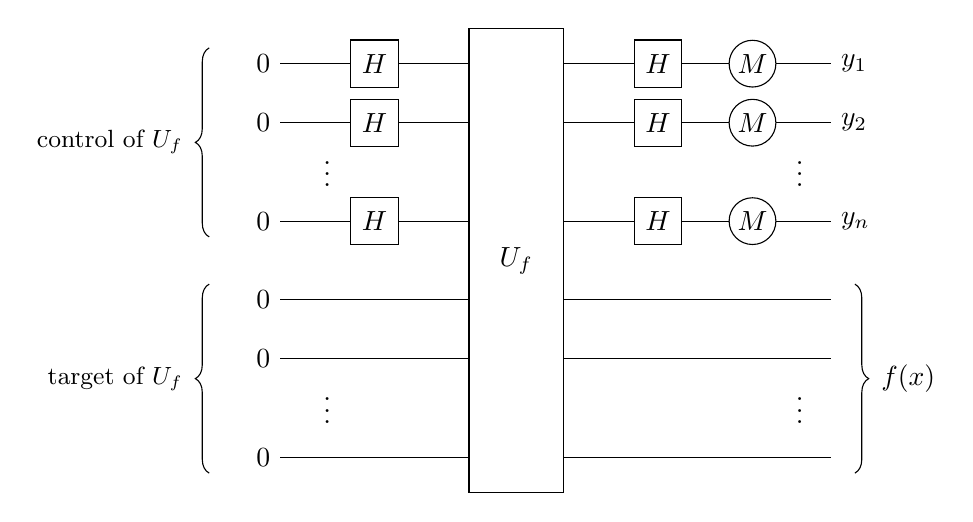
\begin{tikzpicture}[
            gate/.style={draw, fill=white, minimum size=6mm, inner sep=1pt},
            meter/.style={draw, circle, fill=white, inner sep=1.5pt},
        ]
        % control register
        \foreach \y in {4,3.25,2} {\draw (0,\y) -- (7,\y); \node[left] at (0,\y) {$\ket{0}$};}
        \node at (0.6,2.7) {$\vdots$};
        \node at (6.6,2.7) {$\vdots$};
        % target register
        \foreach \y in {1,0.25,-1} {\draw (0,\y) -- (7,\y); \node[left] at (0,\y) {$\ket{0}$};}
        \node at (0.6,-0.3) {$\vdots$};
        \node at (6.6,-0.3) {$\vdots$};
        % query
        \draw[fill=white] (2.4,-1.45) rectangle (3.6,4.45);
        \node at (3,1.5) {$U_f$};
        % Hadamard gates and measurements on the control register
        \foreach \y in {4,3.25,2} {
                \node[gate] at (1.2,\y) {$H$};
                \node[gate] at (4.8,\y) {$H$};
                \node[meter] at (6,\y) {$M$};
            }
        \node[right] at (7,4) {$y_1$};
        \node[right] at (7,3.25) {$y_2$};
        \node[right] at (7,2) {$y_n$};
        \draw[decorate, decoration={brace, amplitude=5pt, mirror}] (7.3,-1.2) -- (7.3,1.2)
        node[midway, right=6pt] {$\ket{f(x)}$};
        \draw[decorate, decoration={brace, amplitude=5pt}] (-0.9,1.8) -- (-0.9,4.2)
        node[midway, left=6pt] {\small control of $U_f$};
        \draw[decorate, decoration={brace, amplitude=5pt}] (-0.9,-1.2) -- (-0.9,1.2)
        node[midway, left=6pt] {\small target of $U_f$};
    \end{tikzpicture}
    \caption{Simon's circuit. The target register is not measured.}
    \label{fig:simon-0929}
\end{figure}

\subsection{Analysis of One Run}

\begin{theorem}[One Run of Simon's Circuit]\label{thm:simon-run-0929}
    Let $y$ be the string measured by the circuit of \cref{fig:simon-0929}.
    \begin{enumerate}
        \item If $f$ is $2$-to-$1$ with period $s \neq 0^n$, then $y$ is uniformly distributed over the
              $2^{n-1}$ strings $y$ with $s \cdot y = 0$: each of them has probability $\sfrac{1}{2^{n-1}}$,
              and every $y$ with $s \cdot y = 1$ has probability $0$.
        \item If $f$ is $1$-to-$1$, then $y$ is uniformly distributed over all of $\set{0,1}^n$: each
              string has probability $\sfrac{1}{2^n}$.
    \end{enumerate}
\end{theorem}

\begin{proof}
    By \cref{lem:wh-0924}, the first layer of Hadamard gates gives
    $\frac{1}{\sqrt{2^n}} \sum_{x} \ket{x}\ket{0^n}$. The query $U_f$ turns this into
    $\frac{1}{\sqrt{2^n}} \sum_{x} \ket{x}\ket{f(x)}$. The second layer of Hadamard gates on the
    control register (\cref{lem:wh-0924} applied to every $\ket{x}$) gives
    \begin{equation}\label{eq:simon-final-0929}
        \frac{1}{2^n} \sum_{y \in \set{0,1}^n} \sum_{x \in \set{0,1}^n} (-1)^{x \cdot y} \ket{y}\ket{f(x)}.
    \end{equation}
    The amplitude $\alpha_{y,z}$ of a basis state $\ket{y}\ket{z}$ collects the $x$ with $f(x) = z$.
    Measuring only the first register gives $y$ with probability $\sum_{z} \abs{\alpha_{y,z}}^2$
    (the probabilities of all basis states $\ket{y}\ket{z}$ with this $y$ add up).

    \emph{Case 2: $f$ is $1$-to-$1$.} The $2^n$ strings $f(x)$ are all different, so every basis state
    $\ket{y}\ket{f(x)}$ appears exactly once in \cref{eq:simon-final-0929}, with amplitude
    $\frac{1}{2^n} (-1)^{x \cdot y}$. So $y$ has probability
    $\sum_{x} \abs{\frac{1}{2^n} (-1)^{x \cdot y}}^2 = 2^n \cdot \frac{1}{2^{2n}} = \frac{1}{2^n}$.

    \emph{Case 1: $f$ is $2$-to-$1$ with period $s \neq 0^n$.} The range $R$ of $f$ has
    $\abs{R} = 2^{n-1}$ elements. For every $z \in R$ let $x_z$ be one of its two preimages; the other
    is $x_z \oplus s$. Because $(x_z \oplus s) \cdot y = x_z \cdot y \oplus s \cdot y$, the amplitude of
    $\ket{y}\ket{z}$ in \cref{eq:simon-final-0929} is
    \[\frac{1}{2^n} \left((-1)^{x_z \cdot y} + (-1)^{(x_z \oplus s) \cdot y}\right)
        = \frac{1}{2^n} (-1)^{x_z \cdot y} \left(1 + (-1)^{s \cdot y}\right)\]
    for $z \in R$ (and $0$ for $z \notin R$). So $y$ has probability
    \[\sum_{z \in R} \abs{\frac{1}{2^n} \left(1 + (-1)^{s \cdot y}\right)}^2
        = 2^{n-1} \cdot \frac{\left(1 + (-1)^{s \cdot y}\right)^2}{2^{2n}}
        = \begin{cases}
            \sfrac{1}{2^{n-1}} & \text{if } s \cdot y = 0, \\
            0                  & \text{if } s \cdot y = 1.
        \end{cases}\]
    There are $2^{n-1}$ strings $y$ with $s \cdot y = 0$, because the pairing $y \mapsto y \oplus e_i$
    of the proof of \cref{lem:signsum-0929}, with $s_i = 1$, matches every $y$ with $s \cdot y = 0$ to
    a $y'$ with $s \cdot y' = 1$.
\end{proof}

\subsection{From the Measurements to \texorpdfstring{$s$}{s}}

Each run of the circuit gives a random $y$ with $s \cdot y = 0$, which is one linear equation
$s_1 y_1 \oplus s_2 y_2 \oplus \dots \oplus s_n y_n = 0$ for the unknown bits $s_1, \dots, s_n$. Running
the circuit $n - 1$ times gives a homogeneous system
\[y_1 \cdot s = 0, \quad y_2 \cdot s = 0, \quad \dots, \quad y_{n-1} \cdot s = 0\]
of linear equations over the field $\set{0,1}$ (addition is $\oplus$). If $y_1, \dots, y_{n-1}$ are
\emph{linearly independent} over $\set{0,1}$, the system has rank $n - 1$. Then its solution space has
dimension $n - (n-1) = 1$ and consists of $0^n$ and one nonzero string $s'$. Gaussian elimination over
$\set{0,1}$ tests the independence and computes $s'$ in $\bigO{n^3}$ time. The true $s$ satisfies every
equation. So if $s \neq 0^n$, at most $n - 1$ of them can be independent, and $n - 1$ independent ones
are enough: if the $y_i$ are independent and $f$ is $2$-to-$1$, then $s' = s$.

\begin{algorithm}[ht]
    \caption{Simon's algorithm}
    \label{alg:simon-0929}
    \begin{algorithmic}[1]
        \State run the circuit of \cref{fig:simon-0929} $n - 1$ times; let $y_1, \dots, y_{n-1}$ be the measured strings
        \If{$y_1, \dots, y_{n-1}$ are linearly dependent over $\set{0,1}$} \Comment{Gaussian elimination}
        \State \Return \textsc{fail}
        \EndIf
        \State let $s'$ be the unique nonzero solution of $y_1 \cdot s' = \dots = y_{n-1} \cdot s' = 0$
        \If{$f(s') = f(0^n)$} \Comment{two classical queries}
        \State \Return $s'$ \Comment{$f$ is $2$-to-$1$ with period $s'$}
        \Else
        \State \Return $0^n$ \Comment{$f$ is $1$-to-$1$}
        \EndIf
    \end{algorithmic}
\end{algorithm}

\begin{theorem}[Simon's Algorithm]\label{thm:simon-0929}
    \cref{alg:simon-0929} makes $n + 1$ queries ($n - 1$ quantum, $2$ classical) and $\bigO{n^3}$ other
    operations. It never outputs a wrong answer, and it outputs the correct $s$ with probability at least
    $\sfrac{1}{4}$.
\end{theorem}

\begin{proof}
    \emph{Never wrong.} If the algorithm does not fail, $y_1, \dots, y_{n-1}$ are independent and $s'$
    is the unique nonzero solution of the system. If $f$ is $2$-to-$1$ with period $s$, then $s$ is a
    nonzero solution, so $s' = s$. The test $f(s') = f(0^n) = f(0^n \oplus s)$ succeeds, and the output
    $s' = s$ is correct. If $f$ is $1$-to-$1$, then $f(s') \neq f(0^n)$ because $s' \neq 0^n$, and the
    output $0^n = s$ is correct.

    \emph{Success probability.} The algorithm fails only if the $y_i$ are dependent. The $n - 1$ runs are
    independent (the registers are re-initialized to $\ket{0^n}\ket{0^n}$ for every run). By
    \cref{thm:simon-run-0929}, the $y_i$ are independent uniform samples from the $2^{n-1}$ strings with
    $s \cdot y = 0$ if $f$ is $2$-to-$1$, and from all of $\set{0,1}^n$ if $f$ is $1$-to-$1$. By
    \cref{thm:indep-1001} (next lecture) they are linearly independent with probability
    \[\left(1 - \frac{1}{2}\right)\left(1 - \frac{1}{2^2}\right)\left(1 - \frac{1}{2^3}\right) \cdots \left(1 - \frac{1}{2^{n-1}}\right) \geq \frac{1}{4}\]
    in the first case and at least $\sfrac{1}{2}$ in the second.
\end{proof}

\subsection{A Deterministic Classical Algorithm}

\begin{exercisebox}
\begin{exercise}\label{ex:simon-det-0929}
    Find a deterministic classical algorithm for Simon's problem that makes $\bigO{\sqrt{2^n}}$ queries.
\end{exercise}
\tcblower
\begin{wsolution}
    We query a set $S$ such that every nonzero string is the XOR of two elements of $S$. A collision
    in $S$ then gives $s$. Let $m = \ceil{n/2}$ and write every $n$-bit string as $x = (u, v)$ with
    $u \in \set{0,1}^m$ its first $m$ bits and $v \in \set{0,1}^{n-m}$ its last $n - m$ bits. Let
    \[S_1 = \set{(u, 0^{n-m}) \suchthat u \in \set{0,1}^m}, \qquad
        S_2 = \set{(0^m, v) \suchthat v \in \set{0,1}^{n-m}}, \qquad
        S = S_1 \cup S_2.\]

    \emph{The algorithm.} Query $f$ on every $x \in S$. If there are $x \neq x'$ in $S$ with
    $f(x) = f(x')$, output $s = x \oplus x'$. Otherwise output $s = 0^n$.

    \emph{Queries.} Because $n - m \leq m \leq \sfrac{(n+1)}{2}$, the algorithm makes
    $\abs{S} \leq 2^m + 2^{n-m} \leq 2 \cdot 2^{m} \leq 2 \cdot 2^{(n+1)/2} = 2\sqrt{2} \cdot \sqrt{2^n}
        = \bigO{\sqrt{2^n}}$ queries, and it is deterministic.

    \emph{Claim: every $s \neq 0^n$ is the XOR of two different elements of $S$.} Write $s = (u, v)$. Then
    $(u, 0^{n-m}) \in S_1$, $(0^m, v) \in S_2$ and $(u, 0^{n-m}) \oplus (0^m, v) = s$. The two elements
    are different, because otherwise $u = 0^m$ and $v = 0^{n-m}$, so $s = 0^n$.

    \emph{Correctness.} If $f$ is $2$-to-$1$ with period $s \neq 0^n$, by the claim there are $x \neq x'$
    in $S$ with $x' = x \oplus s$, so $f(x) = f(x')$ and we find a collision. Any collision
    $f(x) = f(x')$ with $x \neq x'$ satisfies $x' = x \oplus s$ by the promise, so the output
    $x \oplus x' = s$ is correct. If $f$ is $1$-to-$1$ there is no
    collision, and the output $0^n = s$ is correct.
\end{wsolution}
\end{exercisebox}


\newlecture{October 1, 2026}{Classical Query Complexity of Simon's Problem, Yao's Minmax
    Principle, Linear Independence in Simon's Algorithm}
In this lecture, we show that the \emph{classical} query complexity of Simon's problem is
$\bigTh{\sqrt{N}}$, where $N = 2^n$, and that the strings measured by Simon's quantum algorithm are
linearly independent with probability at least $\sfrac{1}{4}$.

\section{Simon's Problem, Classically}

In Simon's problem, $f \colon \set{0,1}^n \to \set{0,1}^n$ is given as a black box with the promise
\[f(x) = f(y) \iff x = y \ \text{ or } \ x \oplus y = s,\]
and we have to find $s$ ($f$ is $1$-to-$1$ if $s = 0^n$ and $2$-to-$1$ with period $s$ otherwise).
Let $N = 2^n$. A classical algorithm learns $f$ only through queries $f(q_1), f(q_2), \dots$, and we
may assume that it never queries the same input twice. A \emph{collision} is a pair of queries
$q_i \neq q_j$ with $f(q_i) = f(q_j)$. By the promise a collision gives $s = q_i \oplus q_j$.

\subsection{Deterministic Algorithms}

\Cref{ex:simon-det-0929} gives a deterministic algorithm with $\bigO{\sqrt{N}}$ queries. This is
optimal by \cref{thm:simon-det-lb-1001}.

\subsection{A Randomized Algorithm}

We query random inputs and wait for a collision.

\begin{algorithm}[ht]
    \caption{Randomized classical algorithm for Simon's problem}
    \label{alg:simon-rand-1001}
    \begin{algorithmic}[1]
        \State choose $k$ distinct inputs $q_1, \dots, q_k$ uniformly at random (without replacement) and query them
        \If{$f(q_i) = f(q_j)$ for some $i \neq j$}
        \State \Return $q_i \oplus q_j$
        \Else
        \State \Return $0^n$
        \EndIf
    \end{algorithmic}
\end{algorithm}

\begin{theorem}[Randomized Upper Bound]\label{thm:simon-rand-ub-1001}
    If $f$ is $1$-to-$1$, \cref{alg:simon-rand-1001} is always correct. If $f$ is $2$-to-$1$ with period
    $s$, it is wrong with probability at most $e^{-k(k-1)/(2N)}$. So with
    $k \geq \sqrt{2N \ln N} + 1$ queries (an integer at most $N$ once $n \geq 3$) the algorithm is correct
    with probability at least $1 - \sfrac{1}{N}$. With $k \geq \sqrt{2N} + 1$ queries, which is
    $\bigO{\sqrt{N}}$, this probability is at least $1 - \sfrac{1}{e}$.
\end{theorem}

\begin{proof}
    If $f$ is $1$-to-$1$ there is no collision, and the output $0^n$ is correct. Let $f$ be $2$-to-$1$
    with period $s \neq 0^n$. The algorithm is wrong only if no collision occurs. Call $q_j \oplus s$
    the \emph{mirror} of $q_j$. A collision occurs at step $i$ exactly when $q_i$ is the mirror of an
    earlier query.

    Suppose that no collision occurred among $q_1, \dots, q_{i-1}$. Their $i - 1$ mirrors are distinct,
    and none is among $q_1, \dots, q_{i-1}$, because that would be a collision. Then all of them are
    among the $N - (i-1)$ inputs not yet queried, and $q_i$ is uniform among those. So the
    probability of a collision at step $i$, given none before, is
    $\sfrac{(i-1)}{(N-i+1)} \geq \sfrac{(i-1)}{N}$. Multiplying over the $k$ steps and using
    $1 - x \leq e^{-x}$,
    \begin{align*}
        \prob{\text{no collision among } q_1, \dots, q_k}
         & \leq \prod_{i=1}^{k} \left(1 - \frac{i-1}{N}\right)
        \leq e^{-\sum_{i=1}^{k} (i-1)/N} \\
         & = e^{-k(k-1)/(2N)} \leq e^{-(k-1)^2/(2N)}.
    \end{align*}
    With $k - 1 \geq \sqrt{2N \ln N}$ this is at most $e^{-\ln N} = \sfrac{1}{N}$, and with
    $k - 1 \geq \sqrt{2N}$ it is at most $e^{-1}$.
\end{proof}

\subsection{Lower Bound for Randomized Algorithms via Yao's Principle}

\begin{theorem}[Randomized Lower Bound]\label{thm:simon-rand-lb-1001}
    Let $n \geq 2$. Every randomized classical algorithm that solves Simon's problem with success
    probability at least $\sfrac{2}{3}$ on every input makes more than $\sfrac{\sqrt{N}}{2}$ queries on
    some input. So every such algorithm needs $\bigOm{\sqrt{N}} = \bigOm{\sqrt{2^n}}$ queries.
\end{theorem}

\begin{lemma}[Yao's Minmax Principle, Easy Direction]\label{lem:yao-1001}
    Let $\mu$ be a probability distribution on the inputs. If every deterministic algorithm that makes at
    most $k$ queries errs with probability greater than $\delta$ on an input drawn from $\mu$, then every
    randomized algorithm that makes at most $k$ queries errs with probability greater than $\delta$ on
    some input.
\end{lemma}

\begin{proof}
    A randomized algorithm $R$ is a deterministic algorithm $A_r$ with at most $k$ queries for every
    fixed random string $r$. Let $\mathrm{err}(A, x) \in \set{0, 1}$ indicate that $A$ is wrong on
    input $x$. Then
    \[\max_{x} \prob[r]{\mathrm{err}(A_r, x) = 1}
        \geq \expectation[x \sim \mu]{\prob[r]{\mathrm{err}(A_r, x) = 1}}
        = \expectation[r]{\prob[x \sim \mu]{\mathrm{err}(A_r, x) = 1}}
        > \delta,\]
    since a maximum is at least an average, the two expectations can be exchanged, and every inner
    probability on the right is greater than $\delta$ by assumption.
\end{proof}

\paragraph{The input distribution.} Let $\mathcal{D}$ be the following distribution of $2$-to-$1$
functions. Choose $s$ uniformly among the $N - 1$ nonzero strings. This splits $\set{0,1}^n$ into
$\sfrac{N}{2}$ pairs $\set{x, x \oplus s}$. Assign distinct values to the pairs, uniformly at
random among all such assignments.

\paragraph{Principle of deferred decisions.} We generate the input lazily. Choose $s$. When the
algorithm queries $q_i$: if $q_i = q_j \oplus s$ for an earlier query $q_j$ (a collision), answer
$f(q_j)$. Otherwise answer a uniformly random value among those not used so far ($N - (i-1)$ of them
as long as no collision has occurred). This produces $\mathcal{D}$, because a uniformly random
injective assignment can be built one value at a time, each uniform among the unused ones.

\begin{lemma}[Few Queries Rarely Collide]\label{lem:collision-1001}
    Let $n \geq 2$ and let $A$ be a deterministic algorithm that makes $k \leq \sfrac{\sqrt{N}}{2}$
    queries, all different, on an input drawn from $\mathcal{D}$.
    \begin{enumerate}
        \item The probability that two of the queries form a pair $\set{x, x \oplus s}$ (a collision)
              is at most
              \[\sum_{i=1}^{k} \frac{i-1}{N - 1 - \binom{i-1}{2}} \leq \frac{k(k-1)}{N}.\]
        \item Given that there is no collision among the $k$ queries, and given the $k$ answers, $s$ is
              uniformly distributed over a set of at least $\sfrac{N}{2}$ strings.
    \end{enumerate}
\end{lemma}

\begin{proof}
    Let $Q_i$ be the event that there is no collision among the first $i$ queries, and $C_i$ the
    event $q_i \oplus s \in \set{q_1, \dots, q_{i-1}}$ that the $\nth{i}$ query collides with an
    earlier one.

    \emph{What the algorithm knows about $s$.} Fix $i \leq k + 1$ and condition on $Q_{i-1}$ and on the
    (distinct) answers $f(q_1), \dots, f(q_{i-1})$. Since $A$ is deterministic, the queries
    $q_1, \dots, q_{i-1}$ are the same for every $s$ that leads to these answers. By the lazy
    generation, this sequence of answers has probability $\prod_{j=1}^{i-1} \sfrac{1}{(N - j + 1)}$, the
    same for every $s$ not of the form $q_j \oplus q_l$ with $j < l \leq i - 1$. It is $0$ for an $s$
    of this form ($q_j$ and $q_l$ would have collided). By Bayes' rule, given the answers, $s$ is
    uniform over the nonzero strings that are not among the at most $\binom{i-1}{2}$ strings
    $q_j \oplus q_l$. This is a set of at least $N - 1 - \binom{i-1}{2} \geq N - 1 - \sfrac{k^2}{2} \geq
        N - 1 - \sfrac{N}{8} \geq \sfrac{N}{2}$ candidates (as $i - 1 \leq k \leq \sfrac{\sqrt{N}}{2}$
    and $N \geq 4$). For $i = k + 1$ this is part~2.

    \emph{Part 1.} If $C_i$ is the first collision then $Q_{i-1}$ holds, so by the union bound
    $\prob{\text{collision}} \leq \sum_{i=1}^{k} \prob{C_i \cap Q_{i-1}}$. Given $Q_{i-1}$ and the answers,
    $q_i$ is determined, and $C_i$ occurs exactly when $s$ is one of the $i - 1$ strings
    $q_i \oplus q_1, \dots, q_i \oplus q_{i-1}$. Averaging over the answers,
    \[\prob{C_i \cap Q_{i-1}} \leq \frac{i-1}{N - 1 - \binom{i-1}{2}} \leq \frac{2(i-1)}{N},
        \qquad \text{so} \qquad
        \prob{\text{collision}} \leq \sum_{i=1}^{k} \frac{2(i-1)}{N} = \frac{k(k-1)}{N}. \qedhere\]
\end{proof}

\begin{proof}[Proof of \cref{thm:simon-rand-lb-1001}]
    Let $A$ be a deterministic algorithm with at most $\sfrac{\sqrt{N}}{2}$ queries. We may assume
    that it never repeats a query and makes the same number $k \leq \sfrac{\sqrt{N}}{2}$ of queries on
    every input, because extra queries whose answers are ignored do not change the output. Run it on
    an input drawn from $\mathcal{D}$. It is correct only if its output is $s$. Suppose there is no
    collision. Given the answers, the output is one fixed string, and $s$ is uniform over at least
    $\sfrac{N}{2}$ strings by part~2 of \cref{lem:collision-1001}. So $A$ is correct with probability
    at most $\sfrac{2}{N}$. With part~1,
    \[\prob{A \text{ correct}} \leq \prob{\text{collision}} + \frac{2}{N} \leq \frac{k(k-1) + 2}{N}.\]
    If $k \geq 2$, then $k(k-1) + 2 \leq k^2 \leq \sfrac{N}{4}$ and the bound is at most $\sfrac{1}{4}$.
    If $k \leq 1$, there is no collision and the bound is $\sfrac{2}{N} \leq \sfrac{1}{2}$. So $A$ errs
    with probability at least $\sfrac{1}{2} > \sfrac{1}{3}$ on $\mathcal{D}$. By \cref{lem:yao-1001}
    with $\mu = \mathcal{D}$ and $\delta = \sfrac{1}{3}$, every randomized algorithm with at most
    $\sfrac{\sqrt{N}}{2}$ queries errs with probability greater than $\sfrac{1}{3}$ on some input.
    So an algorithm with success probability at least $\sfrac{2}{3}$ on every input makes more than
    $\sfrac{\sqrt{N}}{2}$ queries on some input.
\end{proof}

\begin{corollary}[Classical Query Complexity of Simon's Problem]\label{thm:simon-det-lb-1001}
    The classical query complexity of Simon's problem is $\bigTh{\sqrt{N}} = \bigTh{\sqrt{2^n}}$, both
    for deterministic algorithms and for randomized algorithms with constant success probability.
    So Simon's quantum algorithm, with $\bigO{n}$ queries, is exponentially faster than every
    classical algorithm.
\end{corollary}

\begin{proof}
    A deterministic algorithm that is always correct is a randomized algorithm with success
    probability $1 \geq \sfrac{2}{3}$, so \cref{thm:simon-rand-lb-1001} gives the lower bound for both
    kinds. The upper bounds are \cref{ex:simon-det-0929} and \cref{thm:simon-rand-ub-1001} (the
    bound $e^{-(k-1)^2/(2N)}$ in its proof is at most $\sfrac{1}{3}$ for $k \geq \sqrt{2N \ln 3} + 1$).
\end{proof}

\begin{corollary}[Decision Version]\label{cor:simon-decision-1001}
    Let $n \geq 2$. Every randomized classical algorithm that decides, with success probability at
    least $\sfrac{2}{3}$ on every input, whether $f$ is $1$-to-$1$ or $2$-to-$1$ makes more than
    $\sfrac{\sqrt{N}}{2}$ queries on some input.
\end{corollary}

\begin{proof}
    Let $\mathcal{P}$ be the uniform distribution on $1$-to-$1$ functions. Let $\mu$ draw $f$ from
    $\mathcal{P}$ or from
    $\mathcal{D}$ with probability $\sfrac{1}{2}$ each. Let $A$ be a deterministic algorithm with
    $k \leq \sfrac{\sqrt{N}}{2}$ queries, all different, as in the proof of
    \cref{thm:simon-rand-lb-1001}. Its answer is a function of the sequence
    $T = (f(q_1), \dots, f(q_k))$ of answers.

    Let $t = (a_1, \dots, a_k)$ have distinct entries. Under $\mathcal{P}$ every answer is uniform
    among the unused values, so $\prob[\mathcal{P}]{T = t} = \prod_{i=1}^{k} \sfrac{1}{(N - i + 1)}$.
    Under $\mathcal{D}$, let $p_i$ be the probability of a collision at step $i$, given no collision
    before and the answers $a_1, \dots, a_{i-1}$. By the proof of \cref{lem:collision-1001},
    $p_i \leq \sfrac{2(i-1)}{N}$. Without a collision the $\nth{i}$ answer is uniform among the
    $N - i + 1$ unused values. By \cref{lem:prodsum-1001} below,
    \begin{align*}
        \prob[\mathcal{D}]{T = t} \geq \prod_{i=1}^{k} \frac{1 - p_i}{N - i + 1}
         & \geq \left(1 - \sum_{i=1}^{k} \frac{2(i-1)}{N}\right) \prob[\mathcal{P}]{T = t} \\
         & = \left(1 - \frac{k(k-1)}{N}\right) \prob[\mathcal{P}]{T = t}
        \geq \frac{3}{4} \prob[\mathcal{P}]{T = t},
    \end{align*}
    because $k(k-1) \leq k^2 \leq \sfrac{N}{4}$.

    Let $\mathcal{T}$ be the set of sequences on which $A$ answers ``$1$-to-$1$'', and let
    $q = \prob[\mathcal{P}]{T \in \mathcal{T}}$. Sequences with a repeated entry have probability $0$
    under $\mathcal{P}$. Summing over $t \in \mathcal{T}$ gives
    $\prob[\mathcal{D}]{T \in \mathcal{T}} \geq \frac{3}{4} q$. So $A$ is correct on an input drawn from
    $\mu$ with probability at most
    \[\frac{1}{2} q + \frac{1}{2}\left(1 - \frac{3}{4} q\right) = \frac{1}{2} + \frac{q}{8} \leq \frac{5}{8} < \frac{2}{3}.\]
    So $A$ errs with probability at least $\sfrac{3}{8} > \sfrac{1}{3}$ on $\mu$. The claim
    follows from \cref{lem:yao-1001}.
\end{proof}

\begin{lemma}\label{lem:prodsum-1001}
    For $a_1, \dots, a_m \in [0, 1]$, $\prod_{i=1}^{m} (1 - a_i) \geq 1 - \sum_{i=1}^{m} a_i$.
\end{lemma}

\begin{proof}
    We use induction on $m$, with equality for $m = 1$. Multiplying the hypothesis for $m - 1$ by
    $1 - a_m \geq 0$ gives
    \[\prod_{i=1}^{m} (1 - a_i) \geq \left(1 - \sum_{i=1}^{m-1} a_i\right)(1 - a_m)
        = 1 - \sum_{i=1}^{m} a_i + a_m \sum_{i=1}^{m-1} a_i \geq 1 - \sum_{i=1}^{m} a_i. \qedhere\]
\end{proof}

\section{Simon's Algorithm Revisited}

In the state \cref{eq:simon-final-0929} just before the measurement, the probability of measuring
$y$ in the control register is the sum of the squared amplitudes of all basis states
$\ket{y}\ket{z}$ with this $y$. This is the squared norm of the vector that multiplies $\ket{y}$:
\[\prob{y} = \norm{\frac{1}{2^n} \sum_{x \in \set{0,1}^n} (-1)^{x \cdot y} \ket{f(x)}}_2^2.\]

\subsection{The \texorpdfstring{$1$}{1}-to-\texorpdfstring{$1$}{1} Case}

\begin{exercisebox}
\begin{exercise}\label{ex:simon-11-1001}
    Suppose that $f$ is $1$-to-$1$. What is the probability of measuring a given string $y$ in Simon's
    circuit, and do these probabilities add up to $1$?
\end{exercise}
\tcblower
\begin{wsolution}
    If $f$ is $1$-to-$1$, the $2^n$ vectors $\ket{f(x)}$ are distinct basis states, so they are
    orthonormal. The vector multiplying $\ket{y}$ then has $2^n$ orthogonal components, each of
    absolute value $\sfrac{1}{2^n}$. Its squared norm is
    \[\prob{y} = \sum_{x \in \set{0,1}^n} \left(\frac{1}{2^n}\right)^2 = 2^n \cdot \frac{1}{2^{2n}} = \frac{1}{2^n}.\]
    So the measured $y$ is uniformly distributed over $\set{0,1}^n$, and the probabilities add up to
    $2^n \cdot \sfrac{1}{2^n} = 1$.
\end{wsolution}
\end{exercisebox}

\subsection{The \texorpdfstring{$2$}{2}-to-\texorpdfstring{$1$}{1} Case}

If $f$ is $2$-to-$1$ with period $s \neq 0^n$, every $y$ with $s \cdot y = 0$ is measured with
probability $\sfrac{1}{2^{n-1}}$ and every $y$ with $s \cdot y = 1$ with probability $0$
(\cref{thm:simon-run-0929}, case 1). There are $2^{n-1}$ strings with $s \cdot y = 0$, so the
probabilities add up to $2^{n-1} \cdot \sfrac{1}{2^{n-1}} = 1$.

\subsection{Solving for \texorpdfstring{$s$}{s}}

\Cref{alg:simon-0929} runs the circuit $n - 1$ times. In the $2$-to-$1$ case the measured strings
$y_1, \dots, y_{n-1}$ give the system of $n - 1$ linear equations
$s \cdot y_1 = 0, \dots, s \cdot y_{n-1} = 0$ over $\set{0,1}$. If the $y_i$ are linearly independent,
the system has rank $n - 1$, and Gaussian elimination gives its only nonzero solution $s'$. The
algorithm then tests $f(0^n) = f(s')$ with two classical queries. If $f$ is $2$-to-$1$, then $s$
solves the system, so $s' = s$ and the test is true. If $f$ is $1$-to-$1$, the test is false because
$s' \neq 0^n$ (\cref{thm:simon-0929}).

\begin{exercisebox}
\begin{exercise}\label{ex:indep-1001}\label{thm:indep-1001}
    Let $V$ be a subspace of $\set{0,1}^n$ of dimension $d \geq 1$, so $\abs{V} = 2^d$, and let
    $y_1, y_2, \dots$ be independent uniformly random elements of $V$. Show that
    \begin{enumerate}
        \item $y_1, \dots, y_d$ are linearly independent with probability
              \[\prod_{i=1}^{d} \left(1 - \frac{1}{2^i}\right)
                  = \left(1 - \frac{1}{2}\right)\left(1 - \frac{1}{2^2}\right)\left(1 - \frac{1}{2^3}\right) \cdots \left(1 - \frac{1}{2^d}\right)
                  \geq \frac{1}{4},\]
        \item $y_1, \dots, y_{d-1}$ are linearly independent with probability
              $\prod_{i=2}^{d} \left(1 - \sfrac{1}{2^i}\right) \geq \sfrac{1}{2}$.
    \end{enumerate}
    Deduce that the strings $y_1, \dots, y_{n-1}$ of Simon's algorithm are linearly independent with
    probability at least $\sfrac{1}{4}$ in the $2$-to-$1$ case
    ($V = \set{y \suchthat s \cdot y = 0}$, $d = n - 1$) and at least $\sfrac{1}{2}$ in the
    $1$-to-$1$ case ($V = \set{0,1}^n$, $d = n$).
\end{exercise}
\tcblower
\begin{proof}
    Suppose that $y_1, \dots, y_j$ are linearly independent, $0 \leq j < d$. Their span consists of the
    $2^j$ vectors $\sum_{i \leq j} c_i y_i$ with $c_i \in \set{0,1}$, all different by independence,
    and it lies inside $V$. The vector $y_{j+1}$ is uniform over the $2^d$ elements of
    $V$ and independent of $y_1, \dots, y_j$. Then $y_1, \dots, y_{j+1}$ are linearly independent exactly
    when $y_{j+1}$ is not in this span, which has probability $1 - \sfrac{2^j}{2^d} = 1 - 2^{-(d-j)}$.
    Multiplying for $j = 0, \dots, m-1$, the first $m$ vectors are linearly independent with
    probability
    \[\prod_{j=0}^{m-1} \left(1 - \frac{1}{2^{d-j}}\right) = \prod_{i=d-m+1}^{d} \left(1 - \frac{1}{2^i}\right),\]
    which gives the two products for $m = d$ and $m = d - 1$. By \cref{lem:prodsum-1001} and the
    geometric series $\sum_{i \geq 2} 2^{-i} = \sfrac{1}{2}$,
    \[\prod_{i=2}^{d} \left(1 - \frac{1}{2^i}\right) \geq 1 - \sum_{i=2}^{d} \frac{1}{2^i} \geq \frac{1}{2},
        \qquad
        \prod_{i=1}^{d} \left(1 - \frac{1}{2^i}\right) = \frac{1}{2} \prod_{i=2}^{d} \left(1 - \frac{1}{2^i}\right) \geq \frac{1}{4}.\]
    In the $2$-to-$1$ case each $y_i$ is uniform over the $2^{n-1}$ strings with $s \cdot y = 0$
    (\cref{thm:simon-run-0929}). They are the solution set of one nontrivial homogeneous linear
    equation, so they form a subspace of dimension $d = n - 1$, and we take $n - 1 = d$ samples. In
    the $1$-to-$1$ case each $y_i$ is uniform over $\set{0,1}^n$ (\cref{ex:simon-11-1001}), $d = n$,
    and we take $d - 1$ samples.
\end{proof}
\end{exercisebox}


\newlecture{October 6, 2026}{Grover's Search Algorithm, Phase Flip, Diffusion Operator,
    Rotation Analysis}
% In this lecture, we study \emph{Grover's search algorithm} for unstructured search over $N = 2^n$
% inputs. Every Grover iteration is a rotation by the angle $2\theta$ in a two-dimensional plane.

\begin{problem}[Unstructured Search]
    Given $f \colon \set{0,1}^n \to \set{0,1}$ as a black box, find an $x$ with $f(x) = 1$.
\end{problem}

Think of $f$ as a Boolean formula and of $x$ as an assignment. In \emph{unique satisfiability} we are
promised that there is exactly one $x$ with $f(x) = 1$. Let
\[a = \abs{\set{x \suchthat f(x) = 1}}, \qquad b = \abs{\set{x \suchthat f(x) \neq 1}} = N - a\]
% Commented out: not in the lecture notes.
% be the numbers of solutions and of non-solutions. The search is \emph{unstructured}: we know nothing
% about $f$ except what the queries tell us. For $a = 1$ every classical algorithm, deterministic or
% randomized, needs $\bigOm{N}$ queries (lectures of September~1 and~3). Grover's algorithm needs
% $\bigO{\sqrt{N}}$ queries, and $\bigO{\sqrt{N/a}}$ for $a$ solutions.
be the numbers of solutions and of non-solutions. The search is \emph{unstructured}: we know nothing
about $f$ except what the queries tell us.

\section{Grover's Algorithm on Two Qubits}

% Commented out: longer wording of the text that follows.
% Let $n = 2$, $N = 4$, and suppose that the unique solution is $x^* = 10$. We write a state of the two
% qubits as its vector of four amplitudes $(a_{00}, a_{01}, a_{10}, a_{11})$. The algorithm has four
% steps (\cref{fig:grover4-1006}).
Let $n = 2$, $N = 4$, and let the unique solution be $x^* = 10$. A state is its amplitude vector
$(a_{00}, a_{01}, a_{10}, a_{11})$. The algorithm has four steps (\cref{fig:grover4-1006}).

\begin{enumerate}
    \item \emph{Uniform superposition with Hadamard gates:}
          $H^{\otimes 2} \ket{00} = \frac{1}{2}\left(\ket{00} + \ket{01} + \ket{10} + \ket{11}\right)
              = \left(\tfrac{1}{2}, \tfrac{1}{2}, \tfrac{1}{2}, \tfrac{1}{2}\right)$.
    \item \emph{Phase flip.} The query $U_f \colon \ket{x}\ket{c} \mapsto \ket{x}\ket{c \oplus f(x)}$
          with the target qubit in $\frac{1}{\sqrt{2}}(\ket{0} - \ket{1})$ is the phase flip of the
          lecture of September~24, $U_f \colon \ket{x} \mapsto (-1)^{f(x)} \ket{x}$. One query gives
          $\left(\tfrac{1}{2}, \tfrac{1}{2}, -\tfrac{1}{2}, \tfrac{1}{2}\right)$.
    \item \emph{Grover diffusion operator.} Let $\mu = \frac{1}{N} \sum_{x} a_x$ be the mean of the
          amplitudes. The diffusion operator $D$ reflects every amplitude about the mean
          (\emph{inversion about the mean}):
          \[D \colon a_x \longmapsto 2\mu - a_x \qquad \text{for every } x.\]
          Here $\mu = \frac{1}{4}$, so the three non-solutions become $2 \cdot \frac{1}{4} - \frac{1}{2} = 0$
          and the solution becomes $2 \cdot \frac{1}{4} + \frac{1}{2} = 1$. The state is
          $(0, 0, 1, 0) = \ket{10}$, so measuring gives $x^* = 10$ with probability $1$ after a
          single query.
    \item In general, \emph{repeat steps 2 and 3} $k$ times, where $k$ is about $\sqrt{N}$
          (\cref{sec:grover-analysis-1006}).
\end{enumerate}

\begin{figure}[ht]
    \centering
    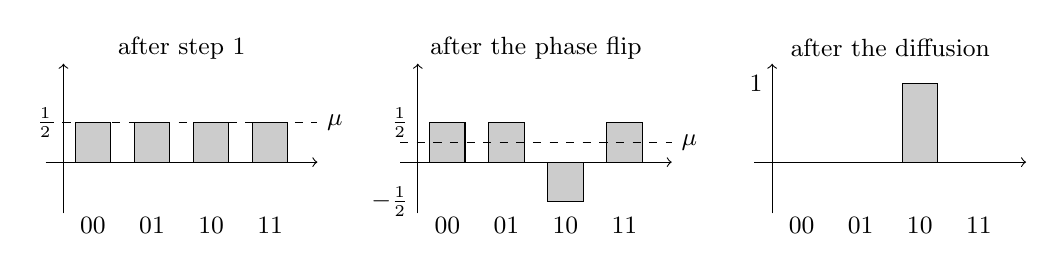
\begin{tikzpicture}[every node/.style={font=\small}, xscale=0.75, yscale=0.5]
        % panel 1
        \begin{scope}
            \draw[->] (-0.3,0) -- (4.3,0);
            \draw[->] (0,-1.3) -- (0,2.5);
            \foreach \x in {0.5,1.5,2.5,3.5} {\draw[fill=gray!40] (\x-0.3,0) rectangle (\x+0.3,1);}
            \foreach \x/\lab in {0.5/00, 1.5/01, 2.5/10, 3.5/11} {\node at (\x,-1.6) {$\lab$};}
            \draw[dashed] (-0.3,1) -- (4.3,1) node[right] {$\mu$};
            \node[left] at (0,1) {$\frac{1}{2}$};
            \node at (2,2.9) {after step 1};
        \end{scope}
        % panel 2
        \begin{scope}[xshift=6cm]
            \draw[->] (-0.3,0) -- (4.3,0);
            \draw[->] (0,-1.3) -- (0,2.5);
            \foreach \x in {0.5,1.5,3.5} {\draw[fill=gray!40] (\x-0.3,0) rectangle (\x+0.3,1);}
            \draw[fill=gray!40] (2.2,0) rectangle (2.8,-1);
            \foreach \x/\lab in {0.5/00, 1.5/01, 2.5/10, 3.5/11} {\node at (\x,-1.6) {$\lab$};}
            \draw[dashed] (-0.3,0.5) -- (4.3,0.5) node[right] {$\mu$};
            \node[left] at (0,1) {$\frac{1}{2}$};
            \node[left] at (0,-1) {$-\frac{1}{2}$};
            \node at (2,2.9) {after the phase flip};
        \end{scope}
        % panel 3
        \begin{scope}[xshift=12cm]
            \draw[->] (-0.3,0) -- (4.3,0);
            \draw[->] (0,-1.3) -- (0,2.5);
            \draw[fill=gray!40] (2.2,0) rectangle (2.8,2);
            \foreach \x/\lab in {0.5/00, 1.5/01, 2.5/10, 3.5/11} {\node at (\x,-1.6) {$\lab$};}
            \node[left] at (0,2) {$1$};
            \node at (2,2.9) {after the diffusion};
        \end{scope}
    \end{tikzpicture}
    \caption{The amplitudes for $N = 4$ and $x^* = 10$ after the Hadamard gates, after the phase flip,
        and after the inversion about the mean $\mu$.}
    \label{fig:grover4-1006}
\end{figure}

\FloatBarrier
\section{Grover's Algorithm on \texorpdfstring{$n$}{n} Qubits}

% Commented out: longer wording of the text that follows.
% For $n$ qubits and a unique solution $x^*$ the same steps apply to the $N$ amplitudes. After the
% Hadamard gates every amplitude is $\sfrac{1}{\sqrt{N}}$. The phase flip makes the amplitude of
% $x^*$ equal to $-\sfrac{1}{\sqrt{N}}$. So the mean is
% $\mu = \sfrac{(N-2)}{(N\sqrt{N})} \approx \sfrac{1}{\sqrt{N}}$ and the diffusion operator maps the
% amplitude of $x^*$ to $2\mu + \sfrac{1}{\sqrt{N}} \approx \sfrac{3}{\sqrt{N}}$. As long as this
% amplitude is small, the mean stays close to $\sfrac{1}{\sqrt{N}}$ and each iteration adds about
% $\sfrac{2}{\sqrt{N}}$ to it. So after about $\sqrt{N}$ iterations it is a constant and a measurement
% finds $x^*$ with constant probability.
For $n$ qubits and a unique solution $x^*$ the same steps apply to the $N$ amplitudes. The Hadamard
gates make every amplitude $\sfrac{1}{\sqrt{N}}$, and the phase flip makes the amplitude of $x^*$
equal to $-\sfrac{1}{\sqrt{N}}$. The mean, and the amplitude of $x^*$ after the diffusion, are
\[\mu = \frac{N-2}{N\sqrt{N}} \approx \frac{1}{\sqrt{N}}, \qquad
    2\mu + \frac{1}{\sqrt{N}} \approx \frac{3}{\sqrt{N}}.\]
While this amplitude is small, the mean stays close to $\sfrac{1}{\sqrt{N}}$ and each iteration adds
about $\sfrac{2}{\sqrt{N}}$ to the amplitude. After about $\sqrt{N}$ iterations it is a constant, and
a measurement finds $x^*$ with constant probability.

\subsection{The Operators \texorpdfstring{$Z_f$}{Zf}, \texorpdfstring{$Z_0$}{Z0} and \texorpdfstring{$D$}{D}}

\paragraph{The phase flip $Z_f$.} The phase flip
\[Z_f \colon \ket{x} \longmapsto (-1)^{f(x)} \ket{x}\]
is implemented by one query $U_f$ with an extra qubit in $H\ket{1} = \frac{1}{\sqrt{2}}(\ket{0} - \ket{1})$
(\cref{fig:zf-1006}). The query leaves the extra qubit unchanged, and a second Hadamard gate returns
it to $\ket{1}$.

\begin{figure}[ht]
    \centering
    \begin{tikzpicture}[scale=0.82, gate/.style={draw, fill=white, minimum size=6mm, inner sep=1pt}]
        \foreach \y in {3,2.25,1} {\draw (0,\y) -- (6,\y);}
        \node at (0.6,1.7) {$\vdots$};
        \node at (5.4,1.7) {$\vdots$};
        \draw (0,-0.25) -- (6,-0.25);
        \node[left] at (0,-0.25) {$\ket{1}$};
        \draw[fill=white] (2.4,-0.7) rectangle (3.6,3.45);
        \node at (3,1.4) {$U_f$};
        \node[gate] at (1.2,-0.25) {$H$};
        \node[gate] at (4.8,-0.25) {$H$};
        \draw[decorate, decoration={brace, amplitude=5pt}] (-0.3,0.8) -- (-0.3,3.2)
        node[midway, left=6pt] {$\ket{x}$};
        \draw[decorate, decoration={brace, amplitude=5pt, mirror}] (6.3,0.8) -- (6.3,3.2)
        node[midway, right=6pt] {$(-1)^{f(x)} \ket{x}$};
        \node[right] at (6.3,-0.25) {$\ket{1}$};
    \end{tikzpicture}
    \caption{The phase flip $Z_f$, implemented with one query $U_f$.}
    \label{fig:zf-1006}
\end{figure}

\paragraph{The phase flip $Z_0$ about $0^n$.} Let $f_0 \colon \set{0,1}^n \to \set{0,1}$ be the function
with $f_0(x) = \bar{x}_1 \wedge \bar{x}_2 \wedge \dots \wedge \bar{x}_n$, where $\bar{x}_i = \neg x_i$,
so $f_0(x) = 1$ only for $x = 0^n$. Its phase flip is
\[Z_0 \colon \ket{x} \longmapsto \begin{cases} -\ket{x} & \text{if } x = 0^n, \\ \ket{x} & \text{otherwise}, \end{cases}
    \qquad \text{so} \qquad Z_0 = I - 2 \ket{0^n}\bra{0^n}.\]
% Commented out: not in the lecture notes.
% As a matrix, $Z_0$ is the $N \times N$ diagonal matrix with $-1$ in the top left corner and $1$
% elsewhere. It is implemented like $Z_f$, with an extra qubit in $H\ket{1}$ and the reversible gate
% $\ket{x}\ket{c} \mapsto \ket{x}\ket{c \oplus (\bar{x}_1 \wedge \dots \wedge \bar{x}_n)}$
% (a Toffoli gate with $n$ negated controls) in place of the black box. It makes no query to $f$.
As a matrix, $Z_0$ is the $N \times N$ diagonal matrix with $-1$ in the top left corner and $1$
elsewhere.

\paragraph{The diffusion operator $D$.} Let $\ket{h} = H^{\otimes n}\ket{0^n} = \frac{1}{\sqrt{N}} \sum_{x} \ket{x}$
be the uniform superposition. The diffusion operator is
\[D = -H^{\otimes n} Z_0 H^{\otimes n}.\]

\begin{lemma}[Inversion About the Mean]\label{lem:diffusion-1006}
    $D = 2\ket{h}\bra{h} - I$, and for every state $\sum_{x} a_x \ket{x}$ with mean amplitude
    $\mu = \frac{1}{N} \sum_{x} a_x$,
    \[D \sum_{x \in \set{0,1}^n} a_x \ket{x} = \sum_{x \in \set{0,1}^n} (2\mu - a_x) \ket{x}.\]
\end{lemma}

\begin{proof}
    Since $H^\dagger = H$ and $H^2 = I$, we have $H^{\otimes n} H^{\otimes n} = I$ and
    $\bra{0^n} H^{\otimes n} = \left(H^{\otimes n}\ket{0^n}\right)^\dagger = \bra{h}$, so
    \[D = -H^{\otimes n} \left(I - 2\ket{0^n}\bra{0^n}\right) H^{\otimes n}
        = -\left(I - 2\ket{h}\bra{h}\right) = 2\ket{h}\bra{h} - I.\]
    For $\ket{\psi} = \sum_x a_x \ket{x}$ we have $\braket{h}{\psi} = \frac{1}{\sqrt{N}} \sum_x a_x = \sqrt{N}\mu$, so
    \[D\ket{\psi} = 2\sqrt{N}\mu \ket{h} - \ket{\psi} = 2\mu \sum_{x} \ket{x} - \sum_{x} a_x \ket{x} = \sum_{x} (2\mu - a_x) \ket{x}. \qedhere\]
\end{proof}

% Commented out: not in the lecture notes.
% So $D$ is the inversion about the mean of step~3, and it makes no query.
So $D$ is the inversion about the mean of step~3.

\paragraph{The Grover iteration.} One iteration of steps 2 and 3 is the operator
\[G = D Z_f = -H^{\otimes n} Z_0 H^{\otimes n} Z_f.\]
Grover's algorithm prepares $\ket{h} = H^{\otimes n}\ket{0^n}$, applies $G$ $k$ times and measures
% Commented out: not in the lecture notes.
% (\cref{fig:grover-circuit-1006}). It makes $k$ queries, one per iteration.
(\cref{fig:grover-circuit-1006}).

\begin{figure}[ht]
    \centering
    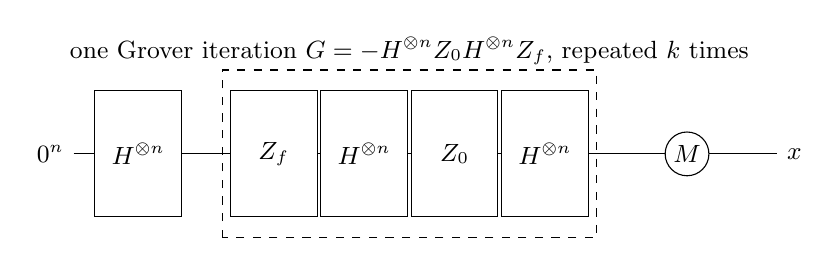
\begin{tikzpicture}[scale=0.82, box/.style={draw, fill=white, minimum height=1.6cm, minimum width=1.1cm, inner sep=2pt},
            meter/.style={draw, circle, fill=white, inner sep=1.5pt}, every node/.style={font=\small}]
        \node[left] at (0,0) {$\ket{0^n}$};
        \draw (0,0) -- (10.9,0);
        \node[box] at (1,0) {$H^{\otimes n}$};
        \node[box] at (3.1,0) {$Z_f$};
        \node[box] at (4.5,0) {$H^{\otimes n}$};
        \node[box] at (5.9,0) {$Z_0$};
        \node[box] at (7.3,0) {$H^{\otimes n}$};
        \node[meter] at (9.5,0) {$M$};
        \draw[dashed] (2.3,-1.3) rectangle (8.1,1.3);
        \node at (5.2,1.6) {one Grover iteration $G = -H^{\otimes n} Z_0 H^{\otimes n} Z_f$, repeated $k$ times};
        \node[right] at (10.9,0) {$x$};
    \end{tikzpicture}
    \caption{Grover's algorithm on $n$ qubits (the extra qubit used by $Z_f$ and $Z_0$ is not drawn).}
    \label{fig:grover-circuit-1006}
\end{figure}

\section{Analysis: A Rotation in Two Dimensions}\label{sec:grover-analysis-1006}

Let $f$ have $a$ solutions, $1 \leq a \leq N - 1$, and let $b = N - a$. Let
\[\ket{A} = \frac{1}{\sqrt{a}} \sum_{\substack{x \in \set{0,1}^n \\ f(x) = 1}} \ket{x},
    \qquad
    \ket{B} = \frac{1}{\sqrt{b}} \sum_{\substack{x \in \set{0,1}^n \\ f(x) = 0}} \ket{x}\]
% Commented out: longer wording of the text that follows.
% be the uniform superpositions of the solutions and of the non-solutions. They are unit vectors, and
% they are orthogonal since no basis state appears in both. The whole computation stays in the plane
% they span. The initial state is
be the uniform superpositions of the solutions and of the non-solutions. They are unit vectors,
orthogonal since no basis state appears in both. The computation stays in their plane. The initial
state is
\begin{equation}\label{eq:h-AB-1006}
    \ket{h} = \frac{1}{\sqrt{N}} \sum_{x \in \set{0,1}^n} \ket{x}
    = \frac{1}{\sqrt{N}} \left(\sqrt{a} \ket{A} + \sqrt{b} \ket{B}\right)
    = \sqrt{\frac{a}{N}} \ket{A} + \sqrt{\frac{b}{N}} \ket{B}.
\end{equation}
Since $\frac{a}{N} + \frac{b}{N} = 1$, there is a unique angle $\theta \in (0, \sfrac{\pi}{2})$ with
\[\sin\theta = \sqrt{\frac{a}{N}}, \qquad \cos\theta = \sqrt{\frac{b}{N}},
    \qquad \text{so that} \qquad \ket{h} = \sin\theta \ket{A} + \cos\theta \ket{B}.\]
For a unique solution, $\sin\theta = \sfrac{1}{\sqrt{N}}$, so $\theta \approx \sfrac{1}{\sqrt{N}}$ and
$\ket{h}$ is almost $\ket{B}$ (\cref{fig:rotation-1006}).

\begin{lemma}[One Grover Iteration]\label{lem:giter-1006}
    \begin{align*}
        G\ket{A} & = \left(1 - \frac{2a}{N}\right)\ket{A} - \frac{2\sqrt{ab}}{N}\ket{B}
        = \cos 2\theta \ket{A} - \sin 2\theta \ket{B},                                 \\
        G\ket{B} & = \frac{2\sqrt{ab}}{N}\ket{A} - \left(1 - \frac{2b}{N}\right)\ket{B}
        = \sin 2\theta \ket{A} + \cos 2\theta \ket{B}.
    \end{align*}
\end{lemma}

\begin{proof}
    % Commented out: longer wording of the text that follows.
    % By the definition of $Z_f$, $Z_f\ket{A} = -\ket{A}$ and $Z_f\ket{B} = \ket{B}$. By
    % \cref{eq:h-AB-1006} and orthonormality, $\braket{h}{A} = \sqrt{a/N}$ and
    % $\braket{h}{B} = \sqrt{b/N}$. With $D = 2\ket{h}\bra{h} - I$ (\cref{lem:diffusion-1006}),
    % substituting \cref{eq:h-AB-1006} for $\ket{h}$ in the last step of each line,
    We have $Z_f\ket{A} = -\ket{A}$ and $Z_f\ket{B} = \ket{B}$. By \cref{eq:h-AB-1006} and
    orthonormality, $\braket{h}{A} = \sqrt{a/N}$ and $\braket{h}{B} = \sqrt{b/N}$. With
    $D = 2\ket{h}\bra{h} - I$ (\cref{lem:diffusion-1006}) and \cref{eq:h-AB-1006} in the last step,
    \begin{align*}
        G\ket{A} = -D\ket{A} & = \ket{A} - 2\ket{h}\braket{h}{A} = \ket{A} - 2\sqrt{\frac{a}{N}} \ket{h}
        = \left(1 - \frac{2a}{N}\right)\ket{A} - \frac{2\sqrt{ab}}{N}\ket{B}, \\
        G\ket{B} = D\ket{B}  & = 2\ket{h}\braket{h}{B} - \ket{B} = 2\sqrt{\frac{b}{N}} \ket{h} - \ket{B}
        = \frac{2\sqrt{ab}}{N}\ket{A} - \left(1 - \frac{2b}{N}\right)\ket{B}.
    \end{align*}
    % Commented out: longer wording of the text that follows.
    % The trigonometric form follows from $\sin^2\theta = \sfrac{a}{N}$, $\cos^2\theta = \sfrac{b}{N}$ and
    % the double angle formulas: $\cos 2\theta = 1 - 2\sin^2\theta = 1 - \sfrac{2a}{N}$,
    % $\cos 2\theta = 2\cos^2\theta - 1 = -\left(1 - \sfrac{2b}{N}\right)$ and
    % $\sin 2\theta = 2\sin\theta\cos\theta = \sfrac{2\sqrt{ab}}{N}$.
    The trigonometric form follows from $\sin^2\theta = \sfrac{a}{N}$, $\cos^2\theta = \sfrac{b}{N}$ and
    the double angle formulas:
    \begin{align*}
        \cos 2\theta & = 1 - 2\sin^2\theta = 1 - \frac{2a}{N},                 \\
        \cos 2\theta & = 2\cos^2\theta - 1 = -\left(1 - \frac{2b}{N}\right), \\
        \sin 2\theta & = 2\sin\theta\cos\theta = \frac{2\sqrt{ab}}{N}. \qedhere
    \end{align*}
\end{proof}

% Commented out: longer wording of the text that follows.
% Since $a + b = N$, both $1 - \sfrac{2a}{N}$ and $\sfrac{2b}{N} - 1$ equal $\sfrac{(b - a)}{N}$. We write a
% state $\beta\ket{B} + \alpha\ket{A}$ of the plane as the column vector $(\beta, \alpha)^{T}$ in the basis
% $(\ket{B}, \ket{A})$. Then $G$ acts as the $2 \times 2$ matrix
Since $a + b = N$, both $1 - \sfrac{2a}{N}$ and $\sfrac{2b}{N} - 1$ equal $\sfrac{(b - a)}{N}$. Write
$\beta\ket{B} + \alpha\ket{A}$ as the column vector $(\beta, \alpha)^{T}$ in the basis
$(\ket{B}, \ket{A})$. Then $G$ acts as the matrix
\begin{equation}\label{eq:gmatrix-1006}
    G = \begin{pmatrix} \dfrac{b - a}{N} & -\dfrac{2\sqrt{ab}}{N} \\[2ex] \dfrac{2\sqrt{ab}}{N} & \dfrac{b - a}{N} \end{pmatrix}
    = \begin{pmatrix} \cos 2\theta & -\sin 2\theta \\ \sin 2\theta & \cos 2\theta \end{pmatrix},
\end{equation}
% Commented out: longer wording of the text that follows.
% whose columns are the coordinates of $G\ket{B}$ and $G\ket{A}$. This is the rotation matrix
% $R_{\phi} = \left(\begin{smallmatrix} \cos\phi & -\sin\phi \\ \sin\phi & \cos\phi \end{smallmatrix}\right)$
% with $\phi = 2\theta$. So one Grover iteration \emph{rotates} the plane by the angle $2\theta$, from
% $\ket{B}$ towards $\ket{A}$.
whose columns are the coordinates of $G\ket{B}$ and $G\ket{A}$. This is the rotation matrix
$R_{\phi} = \left(\begin{smallmatrix} \cos\phi & -\sin\phi \\ \sin\phi & \cos\phi \end{smallmatrix}\right)$
with $\phi = 2\theta$: one Grover iteration \emph{rotates} the plane by $2\theta$, from $\ket{B}$
towards $\ket{A}$.

\begin{exercisebox}
\begin{exercise}\label{ex:grover-rotation-1006}
    Compute $G\ket{h} = \sqrt{\sfrac{a}{N}}\, G\ket{A} + \sqrt{\sfrac{b}{N}}\, G\ket{B}$ and
    $G^k\ket{h}$ for $k \geq 0$, and verify that the matrix of $G$ in \cref{eq:gmatrix-1006} is the
    rotation $R_{2\theta}$.
\end{exercise}
\tcblower
\begin{wsolution}
    % Commented out: longer wording of the text that follows.
    % \emph{The matrix is a rotation.} By \cref{lem:giter-1006} and $\sfrac{(b-a)}{N} = 1 - \sfrac{2a}{N} = \sfrac{2b}{N} - 1$,
    % the two columns of the matrix in \cref{eq:gmatrix-1006} are the coordinates of
    % $G\ket{B} = \cos 2\theta \ket{B} + \sin 2\theta \ket{A}$ and $G\ket{A} = -\sin 2\theta \ket{B} + \cos 2\theta \ket{A}$,
    % which are the columns of $R_{2\theta}$ (not $R_\theta$).
    \emph{The matrix is a rotation.} By \cref{lem:giter-1006} and
    $\sfrac{(b-a)}{N} = 1 - \sfrac{2a}{N} = \sfrac{2b}{N} - 1$, the columns of the matrix in
    \cref{eq:gmatrix-1006} are the coordinates of
    \[G\ket{B} = \cos 2\theta \ket{B} + \sin 2\theta \ket{A}, \qquad
        G\ket{A} = -\sin 2\theta \ket{B} + \cos 2\theta \ket{A}.\]
    These are the columns of $R_{2\theta}$ (not $R_\theta$).

    \emph{The state $G\ket{h}$.} By \cref{eq:h-AB-1006}, $\ket{h} = \sin\theta \ket{A} + \cos\theta \ket{B}$.
    By \cref{lem:giter-1006} and the addition formulas for $\sin(\theta + 2\theta)$ and
    $\cos(\theta + 2\theta)$,
    \begin{align*}
        G\ket{h}
         & = \sin\theta \left(\cos 2\theta \ket{A} - \sin 2\theta \ket{B}\right) + \cos\theta \left(\sin 2\theta \ket{A} + \cos 2\theta \ket{B}\right) \\
         & = \sin 3\theta \ket{A} + \cos 3\theta \ket{B}.
    \end{align*}
    With $\sin 3\theta = 3\sin\theta - 4\sin^3\theta$, $\cos 3\theta = 4\cos^3\theta - 3\cos\theta$ and
    $\sfrac{4b}{N} - 3 = 1 - \sfrac{4a}{N}$, this is
    \[G\ket{h} = \sqrt{\frac{a}{N}}\left(3 - \frac{4a}{N}\right)\ket{A} + \sqrt{\frac{b}{N}}\left(1 - \frac{4a}{N}\right)\ket{B}.\]
    The state starts at the angle $\theta$ from $\ket{B}$ and the iteration adds $2\theta$
    (\cref{fig:rotation-1006}).

    % Commented out: longer wording of the text that follows.
    % \emph{The state $G^k\ket{h}$.} The same computation with any angle $\beta$ in place of $\theta$ gives
    % $G\left(\sin\beta \ket{A} + \cos\beta \ket{B}\right) = \sin(\beta + 2\theta) \ket{A} + \cos(\beta + 2\theta) \ket{B}$.
    % So by induction on $k$, starting from the angle $\theta$ of $\ket{h}$,
    \emph{The state $G^k\ket{h}$.} The same computation with any angle $\beta$ in place of $\theta$ gives
    \[G\left(\sin\beta \ket{A} + \cos\beta \ket{B}\right) = \sin(\beta + 2\theta) \ket{A} + \cos(\beta + 2\theta) \ket{B}.\]
    By induction on $k$, starting from the angle $\theta$ of $\ket{h}$,
    \[G^k\ket{h} = \sin\left((2k+1)\theta\right) \ket{A} + \cos\left((2k+1)\theta\right) \ket{B}.\]
\end{wsolution}
\end{exercisebox}

\begin{figure}[ht]
    \centering
    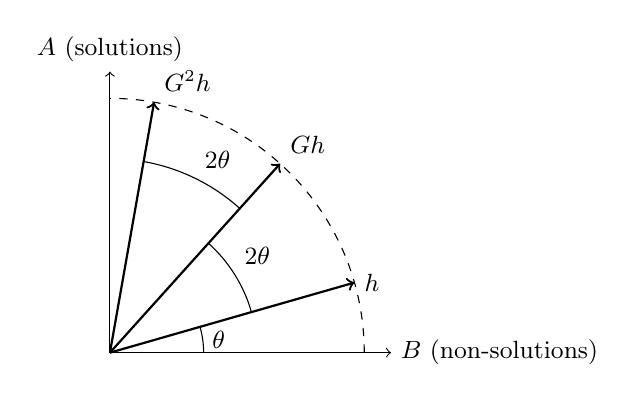
\begin{tikzpicture}[scale=0.85, every node/.style={font=\small}]
        \draw[->] (0,0) -- (4.2,0) node[right] {$\ket{B}$ (non-solutions)};
        \draw[->] (0,0) -- (0,4.2) node[above] {$\ket{A}$ (solutions)};
        \draw[->, thick] (0,0) -- (16:3.8) node[right] {$\ket{h}$};
        \draw[->, thick] (0,0) -- (48:3.8) node[above right] {$G\ket{h}$};
        \draw[->, thick] (0,0) -- (80:3.8) node[above right] {$G^2\ket{h}$};
        \draw (1.4,0) arc (0:16:1.4) node[midway, right] {$\theta$};
        \draw (16:2.2) arc (16:48:2.2) node[midway, above right] {$2\theta$};
        \draw (48:2.9) arc (48:80:2.9) node[midway, above right] {$2\theta$};
        \draw[dashed] (3.8,0) arc (0:90:3.8);
    \end{tikzpicture}
    \caption{Grover's algorithm in the plane spanned by $\ket{A}$ and $\ket{B}$ for
        $\theta = 16^\circ$.}
    \label{fig:rotation-1006}
\end{figure}

The number of iterations is computed in the next lecture (\cref{sec:iterations-1008}).

\FloatBarrier


\newlecture{October 8, 2026}{Grover's Algorithm as Two Reflections, Number of Iterations,
    Random Number of Iterations, Quantum Amplitude Amplification}
In this lecture, we finish the analysis of \emph{Grover's search algorithm}: one iteration is two
\emph{reflections}, which make a rotation. We then choose the number of iterations at
\emph{random} and generalize the algorithm to \emph{quantum amplitude amplification}.

\paragraph{Recap.} We keep the notation of the last lecture ($a$, $b = N - a$ with
$1 \leq a \leq N - 1$, $\ket{A}$, $\ket{B}$, $Z_f$, $Z_0$, $D$, $\ket{h}$ and the Grover iteration
$G = D Z_f = -H^{\otimes n} Z_0 H^{\otimes n} Z_f$; \cref{fig:grover-circuit-1006}). By
\cref{eq:h-AB-1006}, $\ket{h} = \sin\theta \ket{A} + \cos\theta \ket{B}$ with
$\theta = \sin^{-1}\left(\sqrt{\sfrac{a}{N}}\right) \in (0, \sfrac{\pi}{2})$. We write a unit vector
of the plane spanned by $\ket{A}$ and $\ket{B}$ with real coefficients as
$\sin\alpha \ket{A} + \cos\alpha \ket{B}$ and call $\alpha$ its \emph{angle} (measured from $\ket{B}$
towards $\ket{A}$). So $\ket{h}$ has angle $\theta$, and a measurement of the state with angle
$\alpha$ gives a solution with probability $\sin^2\alpha$.

\section{A Grover Iteration Is Two Reflections}

Since $Z_f \ket{A} = -\ket{A}$ and $Z_f \ket{B} = \ket{B}$ (proof of \cref{lem:giter-1006}),
$Z_f \left(\sin\alpha \ket{A} + \cos\alpha \ket{B}\right) = \sin(-\alpha) \ket{A} + \cos(-\alpha) \ket{B}$.
So $Z_f$ is the reflection of the plane about the line of $\ket{B}$.

Let $\ket{h^\perp} = \cos\theta \ket{A} - \sin\theta \ket{B}$. It is a unit vector of the plane with
$\braket{h}{h^\perp} = \sin\theta\cos\theta - \cos\theta\sin\theta = 0$, so $\ket{h}$ and
$\ket{h^\perp}$ are a second orthonormal basis of the plane (\cref{fig:reflections-1008}).

\begin{exercise}\label{ex:diffusion-1008}
    Show that $D = 2\ket{h}\bra{h} - I$, and that for every state
    $\ket{\phi} = c \ket{h} + d \ket{h^\perp}$ of the plane,
    \[D \ket{\phi} = c \ket{h} - d \ket{h^\perp}.\]
\end{exercise}

\begin{wsolution}
    The first claim is \cref{lem:diffusion-1006}: $H^{\otimes n} H^{\otimes n} = I$ and
    $\bra{0^n} H^{\otimes n} = \bra{h}$ give
    \[D = -H^{\otimes n}\left(I - 2\ket{0^n}\bra{0^n}\right)H^{\otimes n} = 2\ket{h}\bra{h} - I.\]
    Since $\braket{h}{h} = 1$ and $\braket{h}{h^\perp} = 0$, we have $\braket{h}{\phi} = c$, so
    \[D\ket{\phi} = 2\ket{h}\braket{h}{\phi} - \ket{\phi} = 2c\ket{h} - c\ket{h} - d\ket{h^\perp}
        = c\ket{h} - d\ket{h^\perp}.\]
    So $D$ is the reflection of the plane about the line of $\ket{h}$.
\end{wsolution}

\paragraph{The sign of $G$.} In class the Grover iteration was also written as
$G = \left(H^{\otimes n} Z_0 H^{\otimes n}\right)\left(-Z_f\right)$, which is the same operator as
$D Z_f = \left(-H^{\otimes n} Z_0 H^{\otimes n}\right) Z_f$ because the minus sign can be moved from
one factor to the other. The form $D Z_f$ is the reflection about
$\ket{B}$ followed by the reflection about $\ket{h}$. In the other form, $-Z_f$ negates the $\ket{B}$
component and $H^{\otimes n} Z_0 H^{\otimes n} = I - 2\ket{h}\bra{h}$ negates the $\ket{h}$
component, so it is the reflection about $\ket{A}$ followed by the reflection about $\ket{h^\perp}$.
Both pairs of lines make the angle $\theta$.

\begin{figure}[ht]
    \centering
    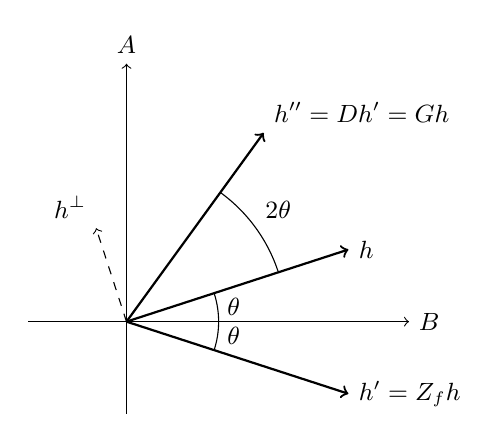
\begin{tikzpicture}[scale=0.78, every node/.style={font=\small}]
        \draw[->] (-1.6,0) -- (4.6,0) node[right] {$\ket{B}$};
        \draw[->] (0,-1.5) -- (0,4.2) node[above] {$\ket{A}$};
        \draw[->, thick] (0,0) -- (18:3.8) node[right] {$\ket{h}$};
        \draw[->, thick] (0,0) -- (-18:3.8) node[right] {$\ket{h'} = Z_f\ket{h}$};
        \draw[->, thick] (0,0) -- (54:3.8) node[above right] {$\ket{h''} = D\ket{h'} = G\ket{h}$};
        \draw[->, dashed] (0,0) -- (108:1.6) node[above left] {$\ket{h^\perp}$};
        \draw (1.5,0) arc (0:18:1.5) node[midway, right] {$\theta$};
        \draw (1.5,0) arc (0:-18:1.5) node[midway, right] {$\theta$};
        \draw (18:2.6) arc (18:54:2.6) node[midway, above right] {$2\theta$};
    \end{tikzpicture}
    \caption{One Grover iteration applied to $\ket{h}$: $Z_f$ reflects about the line of $\ket{B}$,
        then $D$ reflects about the line of $\ket{h}$.}
    \label{fig:reflections-1008}
\end{figure}

\subsection{Two Reflections Make a Rotation}

In \cref{fig:reflections-1008} the first reflection takes the angle $\theta$ to $-\theta$ and the
second, about the line at angle $\theta$, takes $-\theta$ to $3\theta$.

\begin{lemma}[Two Reflections Make a Rotation]\label{lem:tworef-1008}
    Let $\ket{A}$ and $\ket{B}$ be orthonormal vectors, let $\theta$ be a real number and
    $\ket{\psi} = \sin\theta \ket{A} + \cos\theta \ket{B}$. Let $S$ be a linear operator with
    $S\ket{A} = -\ket{A}$ and $S\ket{B} = \ket{B}$, and let $T = 2\ket{\psi}\bra{\psi} - I$. Then for
    every real number $\beta$,
    \[T S \left(\sin\beta \ket{A} + \cos\beta \ket{B}\right)
        = \sin(\beta + 2\theta) \ket{A} + \cos(\beta + 2\theta) \ket{B},\]
    and so, for every integer $k \geq 0$,
    \[(TS)^k \ket{\psi} = \sin\left((2k+1)\theta\right) \ket{A} + \cos\left((2k+1)\theta\right) \ket{B}.\]
\end{lemma}

\begin{proof}
    By linearity, $S(\sin\beta \ket{A} + \cos\beta \ket{B}) = -\sin\beta \ket{A} + \cos\beta \ket{B}
        = \sin\gamma \ket{A} + \cos\gamma \ket{B} =: \ket{\chi}$ with $\gamma = -\beta$. By orthonormality,
    $\braket{\psi}{\chi} = \sin\theta\sin\gamma + \cos\theta\cos\gamma = \cos(\gamma - \theta)$, so
    \begin{align*}
        T\ket{\chi} & = 2\cos(\gamma - \theta)\ket{\psi} - \ket{\chi}                                     \\
                    & = \left(2\cos(\gamma - \theta)\sin\theta - \sin\gamma\right)\ket{A}
        + \left(2\cos(\gamma - \theta)\cos\theta - \cos\gamma\right)\ket{B}.
    \end{align*}
    By the product formulas $2\cos u \sin v = \sin(u + v) - \sin(u - v)$ and
    $2\cos u \cos v = \cos(u + v) + \cos(u - v)$ with $u = \gamma - \theta$ and $v = \theta$, the
    coefficients are $-\sin(\gamma - 2\theta) = \sin(2\theta - \gamma)$ and
    $\cos(\gamma - 2\theta) = \cos(2\theta - \gamma)$. So $T$ sends the angle $\gamma$ to
    $2\theta - \gamma$, and $TS$ sends $\beta$ to $2\theta - (-\beta) = \beta + 2\theta$. This is the
    first claim. The state $\ket{\psi}$ has the angle $\theta$ and each application of $TS$ adds
    $2\theta$, so induction on $k$ gives the angle $(2k+1)\theta$ for $(TS)^k\ket{\psi}$.
\end{proof}

For Grover's algorithm we take $S = Z_f$, $\ket{\psi} = \ket{h}$ and $T = D = 2\ket{h}\bra{h} - I$
(\cref{ex:diffusion-1008}), so that $TS = D Z_f = G$:

\begin{corollary}[The State After $k$ Iterations]\label{cor:hk-1008}
    Every Grover iteration rotates the plane by $2\theta$ from $\ket{B}$ towards $\ket{A}$, and the
    state after $k$ iterations is
    \[\ket{h^k} = G^k\ket{h} = \sin\left((2k+1)\theta\right) \ket{A} + \cos\left((2k+1)\theta\right) \ket{B}.\]
    A measurement of $\ket{h^k}$ gives a solution with probability $\sin^2\left((2k+1)\theta\right)$.
\end{corollary}

\subsection{The Matrix of a Grover Iteration}

Let $M$ be the matrix of the Grover iteration in the basis $(\ket{B}, \ket{A})$
(\cref{eq:gmatrix-1006}).

\begin{exercise}\label{ex:msquare-1008}
    Show that
    \[M = \begin{pmatrix} \sqrt{\sfrac{b}{N}} & -\sqrt{\sfrac{a}{N}} \\[1ex] \sqrt{\sfrac{a}{N}} & \sqrt{\sfrac{b}{N}} \end{pmatrix}^{2}
        = \begin{pmatrix} \cos\theta & -\sin\theta \\ \sin\theta & \cos\theta \end{pmatrix}^{2},\]
    that is, the Grover iteration is the rotation by $\theta$ applied twice.
\end{exercise}

\begin{wsolution}
    Let $R_\theta = \left(\begin{smallmatrix} \cos\theta & -\sin\theta \\ \sin\theta & \cos\theta \end{smallmatrix}\right)$
    with $\cos\theta = \sqrt{\sfrac{b}{N}}$ and $\sin\theta = \sqrt{\sfrac{a}{N}}$. Multiplying,
    \[R_\theta^2
        = \begin{pmatrix} \cos^2\theta - \sin^2\theta & -2\sin\theta\cos\theta \\ 2\sin\theta\cos\theta & \cos^2\theta - \sin^2\theta \end{pmatrix}
        = \begin{pmatrix} \dfrac{b - a}{N} & -\dfrac{2\sqrt{ab}}{N} \\[2ex] \dfrac{2\sqrt{ab}}{N} & \dfrac{b - a}{N} \end{pmatrix} = M,\]
    and by the double angle formulas the middle matrix is $R_{2\theta}$. So $M^k = R_{2k\theta}$.
    This is \cref{cor:hk-1008} in matrix form: $\ket{h}$ is the first column
    $(\cos\theta, \sin\theta)^T$ of $R_\theta$, so $M^k\ket{h}$ is the first column of $R_{(2k+1)\theta}$.
\end{wsolution}

\section{The Number of Iterations}\label{sec:iterations-1008}

By \cref{cor:hk-1008} we want $(2k+1)\theta \approx \sfrac{\pi}{2}$, so
$k \approx \frac{\pi}{4\theta} - \frac{1}{2}$. With $\theta \approx \sin\theta = \sqrt{\sfrac{a}{N}}$
we take
\[k = \floor{\frac{\pi}{4}\sqrt{\frac{N}{a}}}, \qquad \text{for a unique solution} \quad k = \floor{\frac{\pi}{4}\sqrt{N}}.\]

\begin{exercise}\label{ex:iterations-1008}\label{thm:iterations-1008}
    Let $f$ have $a$ solutions, $1 \leq a \leq \sfrac{N}{2}$, and let
    $\kappa = \frac{\pi}{4}\sqrt{\sfrac{N}{a}}$. Show that Grover's algorithm with $k = \floor{\kappa}$
    iterations makes $k \geq 1$ queries and outputs a solution with probability at least
    $1 - \sfrac{2a}{N}$ (at least $1 - \sfrac{2}{N}$ for a unique solution).
\end{exercise}

\begin{proof}
    Let $t = \frac{\pi}{4\theta} - \frac{1}{2}$, so that $(2t+1)\theta = \sfrac{\pi}{2}$ and
    $(2k+1)\theta = \frac{\pi}{2} + 2(k-t)\theta$ for every integer $k$. By \cref{cor:hk-1008},
    $\sin(\sfrac{\pi}{2} + x) = \cos x$ and $\abs{\sin x} \leq \abs{x}$, the success probability is
    \begin{equation}\label{eq:succ-1008}
        \sin^2\left((2k+1)\theta\right) = \cos^2\left(2(k-t)\theta\right) = 1 - \sin^2\left(2(k-t)\theta\right)
        \geq 1 - 4(k-t)^2\theta^2.
    \end{equation}

    \emph{Two facts about $\theta$.} Since $\sin\theta = \sqrt{\sfrac{a}{N}} \leq \sfrac{1}{\sqrt{2}}$,
    we have $0 < \theta \leq \sfrac{\pi}{4}$, so $\theta < 0.79$ and $\theta^2 < 0.62$. We use
    $\theta - \sfrac{\theta^3}{6} \leq \sin\theta \leq \theta$ for $\theta \geq 0$. The lower bound
    holds because $g(x) = \sin x - x + \sfrac{x^3}{6}$ has $g(0) = 0$ and
    $g'(x) = \cos x - 1 + \sfrac{x^2}{2} \geq 0$, as $1 - \cos x = 2\sin^2(\sfrac{x}{2}) \leq \sfrac{x^2}{2}$.
    So $\sin\theta \geq \theta\left(1 - \sfrac{\theta^2}{6}\right)$ with
    $1 - \sfrac{\theta^2}{6} > 1 - \sfrac{0.62}{6} > 0.896$. First, as $0.896^2 > 0.8$,
    \begin{equation}\label{eq:theta2-1008}
        \theta^2 \leq \frac{\sin^2\theta}{(1 - \sfrac{\theta^2}{6})^2} < \frac{\sin^2\theta}{0.896^2} < \frac{5}{4}\sin^2\theta = \frac{5a}{4N}.
    \end{equation}
    Second, $\kappa = \frac{\pi}{4\sin\theta}$, and
    \[0 \leq \frac{1}{\sin\theta} - \frac{1}{\theta}
        \leq \frac{1}{\theta\left(1 - \sfrac{\theta^2}{6}\right)} - \frac{1}{\theta}
        = \frac{\theta}{6 - \theta^2} < \frac{0.79}{5.38} < 0.15,\]
    so, multiplying by $\sfrac{\pi}{4} < 0.79$, we get
    $0 \leq \kappa - \sfrac{\pi}{4\theta} < 0.79 \cdot 0.15 < \sfrac{1}{8}$. This gives
    $\frac{1}{2} \leq \kappa - t < \frac{5}{8}$.

    \emph{The bound.} For $k = \floor{\kappa}$ we have $-1 < k - \kappa \leq 0$, so
    $-\frac{1}{2} < k - t = (k - \kappa) + (\kappa - t) < \frac{5}{8}$ and
    $(k - t)^2 < \sfrac{25}{64}$. By \cref{eq:succ-1008,eq:theta2-1008} the success probability is at
    least
    \[1 - 4 \cdot \frac{25}{64} \cdot \frac{5a}{4N} = 1 - \frac{125}{64} \cdot \frac{a}{N} \geq 1 - \frac{2a}{N}.\]
    Also $\kappa \geq \frac{\pi}{4}\sqrt{2} > 1$ because $\sfrac{N}{a} \geq 2$, so $k \geq 1$.
\end{proof}

With $\ceil{\kappa}$ instead of $\floor{\kappa}$, the bound fails in general.
For $a = \sfrac{N}{4}$ we have $\theta = \sfrac{\pi}{6}$ and $\kappa = \sfrac{\pi}{2} \approx 1.57$.
Then $\floor{\kappa} = 1$ iteration gives the angle $\sfrac{\pi}{2}$ and success probability $1$,
but $\ceil{\kappa} = 2$ iterations overshoot to $\sfrac{5\pi}{6}$ and success probability $\sfrac{1}{4}$.

\section{A Random Number of Iterations}\label{sec:randomk-1008}

The number of iterations $\floor{\frac{\pi}{4}\sqrt{\sfrac{N}{a}}}$ depends on the number $a$ of
solutions, which we may not know. So we choose $k$ \emph{at random}. Since $\sqrt{N}$ need not be an
integer, the largest value is $\floor{2\sqrt{N}}$.

\begin{exercise}\label{ex:randomk-1008}\label{thm:randomk-1008}
    Let $N = 2^n$, let $f$ have $a$ solutions, $1 \leq a \leq \sfrac{N}{2}$, and let
    $K = \floor{2\sqrt{N}}$. Choose $k$ uniformly at random from $\set{1, \dots, K}$, make $k$ Grover
    iterations on $\ket{h}$ and measure. Prove that the probability of measuring a solution is
    \begin{equation}\label{eq:avg-1008}
        \prob{\text{success}} = \frac{1}{2} - \frac{\sin\left(4(K+1)\theta\right) - \sin 4\theta}{4K\sin 2\theta}
        \geq \frac{1}{2} - \frac{1}{4K\sin 2\theta} \geq \frac{3}{8},
    \end{equation}
    so that $\prob{\text{success}} = \bigTh{1}$ with at most $2\sqrt{N} = \bigO{\sqrt{N}}$ queries.
\end{exercise}

\begin{proof}
    \emph{The average.} Given $k$, the success probability is $\sin^2((2k+1)\theta)$ by
    \cref{cor:hk-1008}, and each value has probability $\sfrac{1}{K}$. By the law of total probability
    and $\sin^2 x = \frac{1}{2}(1 - \cos 2x)$,
    \[\prob{\text{success}} = \frac{1}{K}\sum_{k=1}^{K} \sin^2\left((2k+1)\theta\right)
        = \frac{1}{2} - \frac{1}{2K}\sum_{k=1}^{K} \cos\left((4k+2)\theta\right).\]
    By the product formula $2\cos u \sin v = \sin(u+v) - \sin(u-v)$ with $u = (4k+2)\theta$ and
    $v = 2\theta$, the sum telescopes:
    \[2\sin 2\theta \sum_{k=1}^{K} \cos\left((4k+2)\theta\right)
        = \sum_{k=1}^{K} \left(\sin\left(4(k+1)\theta\right) - \sin\left(4k\theta\right)\right)
        = \sin\left(4(K+1)\theta\right) - \sin 4\theta.\]
    As $\sin\theta = \sqrt{\sfrac{a}{N}} \leq \sfrac{1}{\sqrt{2}}$, we have $0 < \theta \leq \sfrac{\pi}{4}$
    and $\sin 2\theta > 0$, so dividing by $2\sin 2\theta$ gives the equality in \cref{eq:avg-1008}.

    \emph{The lower bound.} $\sin(4(K+1)\theta) \leq 1$, and $\sin 4\theta \geq 0$ because
    $0 < 4\theta \leq \pi$. So the numerator is at most $1$, which gives the first inequality in
    \cref{eq:avg-1008}. Since $b = N - a \geq \sfrac{N}{2}$,
    \[\sin 2\theta = 2\sin\theta\cos\theta = \frac{2\sqrt{ab}}{N} \geq \frac{2\sqrt{a \cdot \sfrac{N}{2}}}{N} = \sqrt{\frac{2a}{N}}.\]
    Next, $\floor{2\sqrt{N}} \geq \sqrt{2N}$ for $N = 2^n$. If $n$ is even, $2\sqrt{N}$ is an integer.
    If $n$ is odd, $\sqrt{2N} = 2^{(n+1)/2}$ is an integer with $\sqrt{2N} \leq 2\sqrt{N}$, so it is at
    most the floor. So $K\sin 2\theta \geq \sqrt{2N} \cdot \sqrt{\sfrac{2a}{N}} = 2\sqrt{a} \geq 2$
    and $\prob{\text{success}} \geq \frac{1}{2} - \frac{1}{8} = \frac{3}{8}$. A probability is at most
    $1$, so $\prob{\text{success}} = \bigTh{1}$. The number of queries is $k \leq K \leq 2\sqrt{N}$.
\end{proof}

For the set $\set{1, \dots, \floor{\sqrt{N}}}$ the same proof with
$K = \floor{\sqrt{N}} \geq \sqrt{\sfrac{N}{2}}$ gives $\prob{\text{success}} \geq \sfrac{1}{4}$.

\section{Quantum Amplitude Amplification}\label{sec:ampamp-1008}

Let $\mathcal{A}$ be any quantum algorithm without measurements (a unitary operator on $n$
qubits), and let $f \colon \set{0,1}^n \to \set{0,1}$ tell us which outcomes $x$ are \emph{good}
($f(x) = 1$) and which are \emph{bad} ($f(x) = 0$). Write
$\mathcal{A}\ket{0^n} = \sum_x c_x \ket{x}$, let
$p = \sum_{x \suchthat f(x) = 1} \abs{c_x}^2$ be the probability that a measurement of
$\mathcal{A}\ket{0^n}$ gives a good outcome, and assume $0 < p < 1$. With the unit vectors
\[\ket{G} = \frac{1}{\sqrt{p}} \sum_{x \suchthat f(x) = 1} c_x \ket{x},
    \qquad
    \ket{B} = \frac{1}{\sqrt{1-p}} \sum_{x \suchthat f(x) = 0} c_x \ket{x},\]
which are orthogonal because no basis state appears in both, the state that $\mathcal{A}$ produces is
$\ket{\phi} = \mathcal{A}\ket{0^n} = \sqrt{p}\, \ket{G} + \sqrt{1-p}\, \ket{B}$. Here $\ket{G}$ is
the good state, unrelated to the Grover iteration $G$.
\emph{Classically} we would run $\mathcal{A}$, measure, check the outcome with $f$, and repeat until
the outcome is good. The number of runs is geometric with mean $\sfrac{1}{p}$.

\begin{exercise}\label{ex:ampamp-1008}\label{thm:ampamp-1008}
    Let $\theta \in (0, \sfrac{\pi}{2})$ with $\sin\theta = \sqrt{p}$, and let
    \[Q = -\mathcal{A} Z_0 \mathcal{A}^{-1} Z_f.\]
    Show that
    $Q^k\ket{\phi} = \sin\left((2k+1)\theta\right)\ket{G} + \cos\left((2k+1)\theta\right)\ket{B}$
    for every $k \geq 0$. Show that for $k = \floor{\sfrac{\pi}{4\theta}}$, a measurement of
    $Q^k\ket{\phi}$ gives a good outcome with probability at least $\max(p, 1 - p) \geq \sfrac{1}{2}$,
    and that computing $Q^k \mathcal{A}\ket{0^n}$ takes
    $2k + 1 \leq \frac{\pi}{2\sqrt{p}} + 1 = \bigO{\sfrac{1}{\sqrt{p}}}$ applications of $\mathcal{A}$ or
    $\mathcal{A}^{-1}$ and $k$ queries to $f$.
\end{exercise}

\begin{proof}
    \emph{The two reflections.} $Z_f$ negates every good basis state and fixes every bad one, so
    $Z_f\ket{G} = -\ket{G}$ and $Z_f\ket{B} = \ket{B}$. Since $\mathcal{A}$ is unitary,
    $\mathcal{A}^{-1} = \mathcal{A}^\dagger$, so $\mathcal{A} I \mathcal{A}^{-1} = I$ and
    $\bra{0^n}\mathcal{A}^{-1} = \left(\mathcal{A}\ket{0^n}\right)^\dagger = \bra{\phi}$. This gives
    \[-\mathcal{A} Z_0 \mathcal{A}^{-1} = -\mathcal{A}\left(I - 2\ket{0^n}\bra{0^n}\right)\mathcal{A}^{-1}
        = -\left(I - 2\ket{\phi}\bra{\phi}\right) = 2\ket{\phi}\bra{\phi} - I.\]
    So $Q = TS$ with $S = Z_f$ and $T = 2\ket{\phi}\bra{\phi} - I$. Also
    $\ket{\phi} = \sin\theta\ket{G} + \cos\theta\ket{B}$ because
    $\cos\theta = \sqrt{1 - \sin^2\theta} = \sqrt{1-p}$.
    \Cref{lem:tworef-1008}, applied to the orthonormal vectors $\ket{G}$ and $\ket{B}$ and to
    $\ket{\psi} = \ket{\phi}$, gives the formula for $Q^k\ket{\phi}$.

    \emph{The success probability.} $\ket{G}$ contains only good basis states and $\ket{B}$ only bad
    ones, so a measurement of $Q^k\ket{\phi}$ gives a good outcome with probability
    $\sin^2((2k+1)\theta)$. For $k = \floor{\sfrac{\pi}{4\theta}}$ we have
    $\sfrac{\pi}{4\theta} - 1 < k \leq \sfrac{\pi}{4\theta}$, so
    $\frac{\pi}{2} - \theta < (2k+1)\theta \leq \frac{\pi}{2} + \theta$. On the interval
    $[\sfrac{\pi}{2} - \theta, \sfrac{\pi}{2} + \theta] \subseteq [0, \pi]$ the sine is at least its
    value at the endpoints, $\sin(\sfrac{\pi}{2} \pm \theta) = \cos\theta$, so the probability is at
    least $\cos^2\theta = 1 - p$. It is also at least $p$: if
    $p \leq \sfrac{1}{2}$ then $1 - p \geq p$, and if $p > \sfrac{1}{2}$ then $\theta > \sfrac{\pi}{4}$,
    so $k = 0$ and the probability is $\sin^2\theta = p$.

    \emph{The cost.} One application of $Q$ uses $\mathcal{A}$ once, $\mathcal{A}^{-1}$ once and $Z_f$
    once (one query to $f$), and $Z_0$ uses neither. Preparing $\ket{\phi}$ uses $\mathcal{A}$ once
    more, so the total is $2k + 1$ applications. Also
    $k \leq \frac{\pi}{4\theta} \leq \frac{\pi}{4\sin\theta} = \frac{\pi}{4\sqrt{p}}$ because
    $\sin\theta \leq \theta$.
\end{proof}


% AI use declaration (required by the course if AI tools were used).
% \clearpage
% \section*{AI Use Declaration}
% TODO: say which tool was used, how it was used, what I modified,
% and give the shareable link of the chat.

% Uncomment if something is cited with \cite{...}.
% \bibliographystyle{abbrv}
% \bibliography{references}
\end{document}
